% Copyright © 2012-2014 Martin Ueding <dev@martin-ueding.de>

% This is my general purpose LaTeX header file for writing German documents.
% Ideally, you include this using a simple ``% Copyright © 2012-2014 Martin Ueding <dev@martin-ueding.de>

% This is my general purpose LaTeX header file for writing German documents.
% Ideally, you include this using a simple ``% Copyright © 2012-2014 Martin Ueding <dev@martin-ueding.de>

% This is my general purpose LaTeX header file for writing German documents.
% Ideally, you include this using a simple ``\input{header.tex}`` in your main
% document and start with ``\title`` and ``\begin{document}`` afterwards.

% If you need to add additional packages, I recommend not doing this in this
% file, but in your main document. That way, you can just drop in a new
% ``header.tex`` and get all the new commands without having to merge manually.

% Since this file encorporates a CC-BY-SA fragment, this whole files is
% licensed under the CC-BY-SA license.

\documentclass[11pt, ngerman, fleqn, DIV=15, headinclude, BCOR=2cm]{scrreprt}

\usepackage{graphicx}

\setkomafont{caption}{\sffamily}
\setkomafont{captionlabel}{\usekomafont{caption}}

%%%%%%%%%%%%%%%%%%%%%%%%%%%%%%%%%%%%%%%%%%%%%%%%%%%%%%%%%%%%%%%%%%%%%%%%%%%%%%%
%                                Locale, date                                 %
%%%%%%%%%%%%%%%%%%%%%%%%%%%%%%%%%%%%%%%%%%%%%%%%%%%%%%%%%%%%%%%%%%%%%%%%%%%%%%%

\usepackage{babel}
\usepackage[iso]{isodate}

%%%%%%%%%%%%%%%%%%%%%%%%%%%%%%%%%%%%%%%%%%%%%%%%%%%%%%%%%%%%%%%%%%%%%%%%%%%%%%%
%                          Margins and other spacing                          %
%%%%%%%%%%%%%%%%%%%%%%%%%%%%%%%%%%%%%%%%%%%%%%%%%%%%%%%%%%%%%%%%%%%%%%%%%%%%%%%

\usepackage[parfill]{parskip}
\usepackage{setspace}
\usepackage[activate]{microtype}

\setlength{\columnsep}{2cm}

%%%%%%%%%%%%%%%%%%%%%%%%%%%%%%%%%%%%%%%%%%%%%%%%%%%%%%%%%%%%%%%%%%%%%%%%%%%%%%%
%                                    Color                                    %
%%%%%%%%%%%%%%%%%%%%%%%%%%%%%%%%%%%%%%%%%%%%%%%%%%%%%%%%%%%%%%%%%%%%%%%%%%%%%%%

\usepackage[usenames, dvipsnames]{xcolor}

\colorlet{darkred}{red!70!black}
\colorlet{darkblue}{blue!70!black}
\colorlet{darkgreen}{green!40!black}

%%%%%%%%%%%%%%%%%%%%%%%%%%%%%%%%%%%%%%%%%%%%%%%%%%%%%%%%%%%%%%%%%%%%%%%%%%%%%%%
%                         Font and font like settings                         %
%%%%%%%%%%%%%%%%%%%%%%%%%%%%%%%%%%%%%%%%%%%%%%%%%%%%%%%%%%%%%%%%%%%%%%%%%%%%%%%

% This replaces all fonts with Bitstream Charter, Bitstream Vera Sans and
% Bitstream Vera Mono. Math will be rendered in Charter.
\usepackage[charter, greekuppercase=italicized]{mathdesign}
\usepackage{beramono}
\usepackage{berasans}

% Bold, sans-serif tensors. This fragment is taken from “egreg” from
% http://tex.stackexchange.com/a/82747/8945 and licensed under `CC-BY-SA
% <https://creativecommons.org/licenses/by-sa/3.0/>`_.
\usepackage{bm}
\DeclareMathAlphabet{\mathsfit}{\encodingdefault}{\sfdefault}{m}{sl}
\SetMathAlphabet{\mathsfit}{bold}{\encodingdefault}{\sfdefault}{bx}{sl}
\newcommand{\tens}[1]{\bm{\mathsfit{#1}}}

% Bold vectors.
\renewcommand{\vec}[1]{\boldsymbol{#1}}

%%%%%%%%%%%%%%%%%%%%%%%%%%%%%%%%%%%%%%%%%%%%%%%%%%%%%%%%%%%%%%%%%%%%%%%%%%%%%%%
%                               Input encoding                                %
%%%%%%%%%%%%%%%%%%%%%%%%%%%%%%%%%%%%%%%%%%%%%%%%%%%%%%%%%%%%%%%%%%%%%%%%%%%%%%%

\usepackage[T1]{fontenc}
\usepackage[utf8]{inputenc}

%%%%%%%%%%%%%%%%%%%%%%%%%%%%%%%%%%%%%%%%%%%%%%%%%%%%%%%%%%%%%%%%%%%%%%%%%%%%%%%
%                         Hyperrefs and PDF metadata                          %
%%%%%%%%%%%%%%%%%%%%%%%%%%%%%%%%%%%%%%%%%%%%%%%%%%%%%%%%%%%%%%%%%%%%%%%%%%%%%%%

\usepackage{hyperref}

% This sets the author in the properties of the PDF as well. If you want to
% change it, just override it with another ``\hypersetup`` call.
\hypersetup{
    breaklinks=false,
    citecolor=darkgreen,
    colorlinks=true,
    linkcolor=darkblue,
    menucolor=black,
    pdfauthor={Martin Ueding},
    urlcolor=darkblue,
}

%%%%%%%%%%%%%%%%%%%%%%%%%%%%%%%%%%%%%%%%%%%%%%%%%%%%%%%%%%%%%%%%%%%%%%%%%%%%%%%
%                               Math Operators                                %
%%%%%%%%%%%%%%%%%%%%%%%%%%%%%%%%%%%%%%%%%%%%%%%%%%%%%%%%%%%%%%%%%%%%%%%%%%%%%%%

% AMS environments like ``align`` and theorems like ``proof``.
\usepackage{amsmath}
\usepackage{amsthm}

% Common math constructs like partial derivatives.
\usepackage{commath}

% Physical units.
\usepackage[output-decimal-marker={,}]{siunitx}

% Since I use mathdesign with italic uppercase greek characters, the Ohm unit will be displayed with an italic Ω by default. Units have to be roman, so this forces it the right way.
\DeclareSIUnit{\ohm}{$\Omegaup$}
\DeclareSIUnit{\division}{DIV}
\DeclareSIUnit{\voltss}{$\mathrm{V_{SS}}$}

% Word like operators.
\DeclareMathOperator{\acosh}{arcosh}
\DeclareMathOperator{\arcosh}{arcosh}
\DeclareMathOperator{\arcsinh}{arsinh}
\DeclareMathOperator{\arsinh}{arsinh}
\DeclareMathOperator{\asinh}{arsinh}
\DeclareMathOperator{\card}{card}
\DeclareMathOperator{\csch}{csch}
\DeclareMathOperator{\diam}{diam}
\DeclareMathOperator{\sech}{sech}
\renewcommand{\Im}{\mathop{{}\mathrm{Im}}\nolimits}
\renewcommand{\Re}{\mathop{{}\mathrm{Re}}\nolimits}

% Fourier transform.
\DeclareMathOperator{\fourier}{\ensuremath{\mathcal{F}}}

% Roman versions of “e” and “i” to serve as Euler's number and the imaginary
% constant.
\newcommand{\eup}{\mathrm e}
\newcommand{\iup}{\mathrm i}

% Symbols for the various mathematical fields (natural numbers, integers,
% rational numbers, real numbers, complex numbers).
\newcommand{\C}{\ensuremath{\mathbb C}}
\newcommand{\N}{\ensuremath{\mathbb N}}
\newcommand{\Q}{\ensuremath{\mathbb Q}}
\newcommand{\R}{\ensuremath{\mathbb R}}
\newcommand{\Z}{\ensuremath{\mathbb Z}}

% Shape like operators.
\DeclareMathOperator{\dalambert}{\Box}
\DeclareMathOperator{\laplace}{\bigtriangleup}
\newcommand{\curl}{\vnabla \times}
\newcommand{\divergence}[1]{\inner{\vnabla}{#1}}
\newcommand{\Divergence}[1]{\Inner{\vnabla}{#1}}
\newcommand{\vnabla}{\vec \nabla}

\newcommand{\half}{\frac 12}

% Unit vector (German „Einheitsvektor“).
\newcommand{\ev}{\hat{\vec e}}

% Mathematician's notation for the inner (scalar, dot) product.
\newcommand{\bracket}[1]{\langle #1 \rangle}
\newcommand{\Bracket}[1]{\left\langle #1 \right\rangle}
\newcommand{\inner}[2]{\bracket{#1, #2}}
\newcommand{\Inner}[2]{\Bracket{#1, #2}}

% Placeholders.
\newcommand{\fehlt}{\textcolor{darkred}{Hier fehlen noch Inhalte.}}
\newcommand{\messwert}{\textcolor{blue}{\square}}
\newcommand{\punkte}{\phantom{xxxxx}}

% Separator for equations on a single line.
\newcommand{\eqnsep}{,\quad}

% Quantum Mechanics.
\usepackage{braket}

% Thermodynamic partial derivative.
\newcommand\tdpd[3]{\del{\dpd{#1}{#2}}_{#3}}

%%%%%%%%%%%%%%%%%%%%%%%%%%%%%%%%%%%%%%%%%%%%%%%%%%%%%%%%%%%%%%%%%%%%%%%%%%%%%%%
%                                  Headings                                   %
%%%%%%%%%%%%%%%%%%%%%%%%%%%%%%%%%%%%%%%%%%%%%%%%%%%%%%%%%%%%%%%%%%%%%%%%%%%%%%%

% This will set fancy headings to the top of the page. The page number will be
% accompanied by the total number of pages. That way, you will know if any page
% is missing.
%
% If you do not want this for your document, you can just use
% ``\pagestyle{plain}``.

\usepackage{scrpage2}

\pagestyle{scrheadings}
\automark{section}
\chead{}
\ihead{}
\ohead{\rightmark}
\setheadsepline{.4pt}

%%%%%%%%%%%%%%%%%%%%%%%%%%%%%%%%%%%%%%%%%%%%%%%%%%%%%%%%%%%%%%%%%%%%%%%%%%%%%%%
%                            Bibliography (BibTeX)                            %
%%%%%%%%%%%%%%%%%%%%%%%%%%%%%%%%%%%%%%%%%%%%%%%%%%%%%%%%%%%%%%%%%%%%%%%%%%%%%%%

\newcommand{\bibliographyfile}{../../central-bibtex/Central}

\usepackage[
    backend=bibtex,
    style=alphabetic,
    %isbn=false,
    %pagetracker=false,
    %maxbibnames=50,
    %maxcitenames=2,
    %autocite=inline,
    %block=space,
    %backref=false,
    %backrefstyle=three+,
    %date=short,
    hyperref=true
]{biblatex}

\setlength{\bibitemsep}{.7em}
\setlength{\bibhang}{4ex}

\IfFileExists{\bibliographyfile}{
    \bibliography{\bibliographyfile}
}{}

%%%%%%%%%%%%%%%%%%%%%%%%%%%%%%%%%%%%%%%%%%%%%%%%%%%%%%%%%%%%%%%%%%%%%%%%%%%%%%%
%                                Abbreviations                                %
%%%%%%%%%%%%%%%%%%%%%%%%%%%%%%%%%%%%%%%%%%%%%%%%%%%%%%%%%%%%%%%%%%%%%%%%%%%%%%%

\newcommand{\dhabk}{\mbox{d.\,h.}}

%%%%%%%%%%%%%%%%%%%%%%%%%%%%%%%%%%%%%%%%%%%%%%%%%%%%%%%%%%%%%%%%%%%%%%%%%%%%%%%
%                                  Licences                                   %
%%%%%%%%%%%%%%%%%%%%%%%%%%%%%%%%%%%%%%%%%%%%%%%%%%%%%%%%%%%%%%%%%%%%%%%%%%%%%%%

\usepackage{ccicons}

\newcommand{\ccbysadetext}{%
    \begin{small}
        Dieses Werk bzw. Inhalt steht unter einer
        \href{http://creativecommons.org/licenses/by-sa/3.0/deed.de}{%
            Creative Commons Namensnennung - Weitergabe unter gleichen
        Bedingungen 3.0 Unported Lizenz}.
    \end{small}
}

\newcommand{\ccbysadetitle}{%
    Lizenz: \href{http://creativecommons.org/licenses/by-sa/3.0/deed.de}
    {CC-BY-SA 3.0 \ccbysa}
}

\newcommand\erklaerungFehlerNotation{%
    In dieser Notation bedeutet \num{1.234 +- 0.005}, dass der Wert
    $\num{1.234} \pm \num{0.005}$ ist. Die Ziffern in Klammern sind die
    Fehlerangabe. Um den Fehler zu erhalten, wird diese von rechts über die
    Zahl gelegt, alle anderen Stellen werden auf 0 gesetzt.
}

`` in your main
% document and start with ``\title`` and ``\begin{document}`` afterwards.

% If you need to add additional packages, I recommend not doing this in this
% file, but in your main document. That way, you can just drop in a new
% ``header.tex`` and get all the new commands without having to merge manually.

% Since this file encorporates a CC-BY-SA fragment, this whole files is
% licensed under the CC-BY-SA license.

\documentclass[11pt, ngerman, fleqn, DIV=15, headinclude, BCOR=2cm]{scrreprt}

\usepackage{graphicx}

\setkomafont{caption}{\sffamily}
\setkomafont{captionlabel}{\usekomafont{caption}}

%%%%%%%%%%%%%%%%%%%%%%%%%%%%%%%%%%%%%%%%%%%%%%%%%%%%%%%%%%%%%%%%%%%%%%%%%%%%%%%
%                                Locale, date                                 %
%%%%%%%%%%%%%%%%%%%%%%%%%%%%%%%%%%%%%%%%%%%%%%%%%%%%%%%%%%%%%%%%%%%%%%%%%%%%%%%

\usepackage{babel}
\usepackage[iso]{isodate}

%%%%%%%%%%%%%%%%%%%%%%%%%%%%%%%%%%%%%%%%%%%%%%%%%%%%%%%%%%%%%%%%%%%%%%%%%%%%%%%
%                          Margins and other spacing                          %
%%%%%%%%%%%%%%%%%%%%%%%%%%%%%%%%%%%%%%%%%%%%%%%%%%%%%%%%%%%%%%%%%%%%%%%%%%%%%%%

\usepackage[parfill]{parskip}
\usepackage{setspace}
\usepackage[activate]{microtype}

\setlength{\columnsep}{2cm}

%%%%%%%%%%%%%%%%%%%%%%%%%%%%%%%%%%%%%%%%%%%%%%%%%%%%%%%%%%%%%%%%%%%%%%%%%%%%%%%
%                                    Color                                    %
%%%%%%%%%%%%%%%%%%%%%%%%%%%%%%%%%%%%%%%%%%%%%%%%%%%%%%%%%%%%%%%%%%%%%%%%%%%%%%%

\usepackage[usenames, dvipsnames]{xcolor}

\colorlet{darkred}{red!70!black}
\colorlet{darkblue}{blue!70!black}
\colorlet{darkgreen}{green!40!black}

%%%%%%%%%%%%%%%%%%%%%%%%%%%%%%%%%%%%%%%%%%%%%%%%%%%%%%%%%%%%%%%%%%%%%%%%%%%%%%%
%                         Font and font like settings                         %
%%%%%%%%%%%%%%%%%%%%%%%%%%%%%%%%%%%%%%%%%%%%%%%%%%%%%%%%%%%%%%%%%%%%%%%%%%%%%%%

% This replaces all fonts with Bitstream Charter, Bitstream Vera Sans and
% Bitstream Vera Mono. Math will be rendered in Charter.
\usepackage[charter, greekuppercase=italicized]{mathdesign}
\usepackage{beramono}
\usepackage{berasans}

% Bold, sans-serif tensors. This fragment is taken from “egreg” from
% http://tex.stackexchange.com/a/82747/8945 and licensed under `CC-BY-SA
% <https://creativecommons.org/licenses/by-sa/3.0/>`_.
\usepackage{bm}
\DeclareMathAlphabet{\mathsfit}{\encodingdefault}{\sfdefault}{m}{sl}
\SetMathAlphabet{\mathsfit}{bold}{\encodingdefault}{\sfdefault}{bx}{sl}
\newcommand{\tens}[1]{\bm{\mathsfit{#1}}}

% Bold vectors.
\renewcommand{\vec}[1]{\boldsymbol{#1}}

%%%%%%%%%%%%%%%%%%%%%%%%%%%%%%%%%%%%%%%%%%%%%%%%%%%%%%%%%%%%%%%%%%%%%%%%%%%%%%%
%                               Input encoding                                %
%%%%%%%%%%%%%%%%%%%%%%%%%%%%%%%%%%%%%%%%%%%%%%%%%%%%%%%%%%%%%%%%%%%%%%%%%%%%%%%

\usepackage[T1]{fontenc}
\usepackage[utf8]{inputenc}

%%%%%%%%%%%%%%%%%%%%%%%%%%%%%%%%%%%%%%%%%%%%%%%%%%%%%%%%%%%%%%%%%%%%%%%%%%%%%%%
%                         Hyperrefs and PDF metadata                          %
%%%%%%%%%%%%%%%%%%%%%%%%%%%%%%%%%%%%%%%%%%%%%%%%%%%%%%%%%%%%%%%%%%%%%%%%%%%%%%%

\usepackage{hyperref}

% This sets the author in the properties of the PDF as well. If you want to
% change it, just override it with another ``\hypersetup`` call.
\hypersetup{
    breaklinks=false,
    citecolor=darkgreen,
    colorlinks=true,
    linkcolor=darkblue,
    menucolor=black,
    pdfauthor={Martin Ueding},
    urlcolor=darkblue,
}

%%%%%%%%%%%%%%%%%%%%%%%%%%%%%%%%%%%%%%%%%%%%%%%%%%%%%%%%%%%%%%%%%%%%%%%%%%%%%%%
%                               Math Operators                                %
%%%%%%%%%%%%%%%%%%%%%%%%%%%%%%%%%%%%%%%%%%%%%%%%%%%%%%%%%%%%%%%%%%%%%%%%%%%%%%%

% AMS environments like ``align`` and theorems like ``proof``.
\usepackage{amsmath}
\usepackage{amsthm}

% Common math constructs like partial derivatives.
\usepackage{commath}

% Physical units.
\usepackage[output-decimal-marker={,}]{siunitx}

% Since I use mathdesign with italic uppercase greek characters, the Ohm unit will be displayed with an italic Ω by default. Units have to be roman, so this forces it the right way.
\DeclareSIUnit{\ohm}{$\Omegaup$}
\DeclareSIUnit{\division}{DIV}
\DeclareSIUnit{\voltss}{$\mathrm{V_{SS}}$}

% Word like operators.
\DeclareMathOperator{\acosh}{arcosh}
\DeclareMathOperator{\arcosh}{arcosh}
\DeclareMathOperator{\arcsinh}{arsinh}
\DeclareMathOperator{\arsinh}{arsinh}
\DeclareMathOperator{\asinh}{arsinh}
\DeclareMathOperator{\card}{card}
\DeclareMathOperator{\csch}{csch}
\DeclareMathOperator{\diam}{diam}
\DeclareMathOperator{\sech}{sech}
\renewcommand{\Im}{\mathop{{}\mathrm{Im}}\nolimits}
\renewcommand{\Re}{\mathop{{}\mathrm{Re}}\nolimits}

% Fourier transform.
\DeclareMathOperator{\fourier}{\ensuremath{\mathcal{F}}}

% Roman versions of “e” and “i” to serve as Euler's number and the imaginary
% constant.
\newcommand{\eup}{\mathrm e}
\newcommand{\iup}{\mathrm i}

% Symbols for the various mathematical fields (natural numbers, integers,
% rational numbers, real numbers, complex numbers).
\newcommand{\C}{\ensuremath{\mathbb C}}
\newcommand{\N}{\ensuremath{\mathbb N}}
\newcommand{\Q}{\ensuremath{\mathbb Q}}
\newcommand{\R}{\ensuremath{\mathbb R}}
\newcommand{\Z}{\ensuremath{\mathbb Z}}

% Shape like operators.
\DeclareMathOperator{\dalambert}{\Box}
\DeclareMathOperator{\laplace}{\bigtriangleup}
\newcommand{\curl}{\vnabla \times}
\newcommand{\divergence}[1]{\inner{\vnabla}{#1}}
\newcommand{\Divergence}[1]{\Inner{\vnabla}{#1}}
\newcommand{\vnabla}{\vec \nabla}

\newcommand{\half}{\frac 12}

% Unit vector (German „Einheitsvektor“).
\newcommand{\ev}{\hat{\vec e}}

% Mathematician's notation for the inner (scalar, dot) product.
\newcommand{\bracket}[1]{\langle #1 \rangle}
\newcommand{\Bracket}[1]{\left\langle #1 \right\rangle}
\newcommand{\inner}[2]{\bracket{#1, #2}}
\newcommand{\Inner}[2]{\Bracket{#1, #2}}

% Placeholders.
\newcommand{\fehlt}{\textcolor{darkred}{Hier fehlen noch Inhalte.}}
\newcommand{\messwert}{\textcolor{blue}{\square}}
\newcommand{\punkte}{\phantom{xxxxx}}

% Separator for equations on a single line.
\newcommand{\eqnsep}{,\quad}

% Quantum Mechanics.
\usepackage{braket}

% Thermodynamic partial derivative.
\newcommand\tdpd[3]{\del{\dpd{#1}{#2}}_{#3}}

%%%%%%%%%%%%%%%%%%%%%%%%%%%%%%%%%%%%%%%%%%%%%%%%%%%%%%%%%%%%%%%%%%%%%%%%%%%%%%%
%                                  Headings                                   %
%%%%%%%%%%%%%%%%%%%%%%%%%%%%%%%%%%%%%%%%%%%%%%%%%%%%%%%%%%%%%%%%%%%%%%%%%%%%%%%

% This will set fancy headings to the top of the page. The page number will be
% accompanied by the total number of pages. That way, you will know if any page
% is missing.
%
% If you do not want this for your document, you can just use
% ``\pagestyle{plain}``.

\usepackage{scrpage2}

\pagestyle{scrheadings}
\automark{section}
\chead{}
\ihead{}
\ohead{\rightmark}
\setheadsepline{.4pt}

%%%%%%%%%%%%%%%%%%%%%%%%%%%%%%%%%%%%%%%%%%%%%%%%%%%%%%%%%%%%%%%%%%%%%%%%%%%%%%%
%                            Bibliography (BibTeX)                            %
%%%%%%%%%%%%%%%%%%%%%%%%%%%%%%%%%%%%%%%%%%%%%%%%%%%%%%%%%%%%%%%%%%%%%%%%%%%%%%%

\newcommand{\bibliographyfile}{../../central-bibtex/Central}

\usepackage[
    backend=bibtex,
    style=alphabetic,
    %isbn=false,
    %pagetracker=false,
    %maxbibnames=50,
    %maxcitenames=2,
    %autocite=inline,
    %block=space,
    %backref=false,
    %backrefstyle=three+,
    %date=short,
    hyperref=true
]{biblatex}

\setlength{\bibitemsep}{.7em}
\setlength{\bibhang}{4ex}

\IfFileExists{\bibliographyfile}{
    \bibliography{\bibliographyfile}
}{}

%%%%%%%%%%%%%%%%%%%%%%%%%%%%%%%%%%%%%%%%%%%%%%%%%%%%%%%%%%%%%%%%%%%%%%%%%%%%%%%
%                                Abbreviations                                %
%%%%%%%%%%%%%%%%%%%%%%%%%%%%%%%%%%%%%%%%%%%%%%%%%%%%%%%%%%%%%%%%%%%%%%%%%%%%%%%

\newcommand{\dhabk}{\mbox{d.\,h.}}

%%%%%%%%%%%%%%%%%%%%%%%%%%%%%%%%%%%%%%%%%%%%%%%%%%%%%%%%%%%%%%%%%%%%%%%%%%%%%%%
%                                  Licences                                   %
%%%%%%%%%%%%%%%%%%%%%%%%%%%%%%%%%%%%%%%%%%%%%%%%%%%%%%%%%%%%%%%%%%%%%%%%%%%%%%%

\usepackage{ccicons}

\newcommand{\ccbysadetext}{%
    \begin{small}
        Dieses Werk bzw. Inhalt steht unter einer
        \href{http://creativecommons.org/licenses/by-sa/3.0/deed.de}{%
            Creative Commons Namensnennung - Weitergabe unter gleichen
        Bedingungen 3.0 Unported Lizenz}.
    \end{small}
}

\newcommand{\ccbysadetitle}{%
    Lizenz: \href{http://creativecommons.org/licenses/by-sa/3.0/deed.de}
    {CC-BY-SA 3.0 \ccbysa}
}

\newcommand\erklaerungFehlerNotation{%
    In dieser Notation bedeutet \num{1.234 +- 0.005}, dass der Wert
    $\num{1.234} \pm \num{0.005}$ ist. Die Ziffern in Klammern sind die
    Fehlerangabe. Um den Fehler zu erhalten, wird diese von rechts über die
    Zahl gelegt, alle anderen Stellen werden auf 0 gesetzt.
}

`` in your main
% document and start with ``\title`` and ``\begin{document}`` afterwards.

% If you need to add additional packages, I recommend not doing this in this
% file, but in your main document. That way, you can just drop in a new
% ``header.tex`` and get all the new commands without having to merge manually.

% Since this file encorporates a CC-BY-SA fragment, this whole files is
% licensed under the CC-BY-SA license.

\documentclass[11pt, ngerman, fleqn, DIV=15, headinclude, BCOR=2cm]{scrreprt}

\usepackage{graphicx}

\setkomafont{caption}{\sffamily}
\setkomafont{captionlabel}{\usekomafont{caption}}

%%%%%%%%%%%%%%%%%%%%%%%%%%%%%%%%%%%%%%%%%%%%%%%%%%%%%%%%%%%%%%%%%%%%%%%%%%%%%%%
%                                Locale, date                                 %
%%%%%%%%%%%%%%%%%%%%%%%%%%%%%%%%%%%%%%%%%%%%%%%%%%%%%%%%%%%%%%%%%%%%%%%%%%%%%%%

\usepackage{babel}
\usepackage[iso]{isodate}

%%%%%%%%%%%%%%%%%%%%%%%%%%%%%%%%%%%%%%%%%%%%%%%%%%%%%%%%%%%%%%%%%%%%%%%%%%%%%%%
%                          Margins and other spacing                          %
%%%%%%%%%%%%%%%%%%%%%%%%%%%%%%%%%%%%%%%%%%%%%%%%%%%%%%%%%%%%%%%%%%%%%%%%%%%%%%%

\usepackage[parfill]{parskip}
\usepackage{setspace}
\usepackage[activate]{microtype}

\setlength{\columnsep}{2cm}

%%%%%%%%%%%%%%%%%%%%%%%%%%%%%%%%%%%%%%%%%%%%%%%%%%%%%%%%%%%%%%%%%%%%%%%%%%%%%%%
%                                    Color                                    %
%%%%%%%%%%%%%%%%%%%%%%%%%%%%%%%%%%%%%%%%%%%%%%%%%%%%%%%%%%%%%%%%%%%%%%%%%%%%%%%

\usepackage[usenames, dvipsnames]{xcolor}

\colorlet{darkred}{red!70!black}
\colorlet{darkblue}{blue!70!black}
\colorlet{darkgreen}{green!40!black}

%%%%%%%%%%%%%%%%%%%%%%%%%%%%%%%%%%%%%%%%%%%%%%%%%%%%%%%%%%%%%%%%%%%%%%%%%%%%%%%
%                         Font and font like settings                         %
%%%%%%%%%%%%%%%%%%%%%%%%%%%%%%%%%%%%%%%%%%%%%%%%%%%%%%%%%%%%%%%%%%%%%%%%%%%%%%%

% This replaces all fonts with Bitstream Charter, Bitstream Vera Sans and
% Bitstream Vera Mono. Math will be rendered in Charter.
\usepackage[charter, greekuppercase=italicized]{mathdesign}
\usepackage{beramono}
\usepackage{berasans}

% Bold, sans-serif tensors. This fragment is taken from “egreg” from
% http://tex.stackexchange.com/a/82747/8945 and licensed under `CC-BY-SA
% <https://creativecommons.org/licenses/by-sa/3.0/>`_.
\usepackage{bm}
\DeclareMathAlphabet{\mathsfit}{\encodingdefault}{\sfdefault}{m}{sl}
\SetMathAlphabet{\mathsfit}{bold}{\encodingdefault}{\sfdefault}{bx}{sl}
\newcommand{\tens}[1]{\bm{\mathsfit{#1}}}

% Bold vectors.
\renewcommand{\vec}[1]{\boldsymbol{#1}}

%%%%%%%%%%%%%%%%%%%%%%%%%%%%%%%%%%%%%%%%%%%%%%%%%%%%%%%%%%%%%%%%%%%%%%%%%%%%%%%
%                               Input encoding                                %
%%%%%%%%%%%%%%%%%%%%%%%%%%%%%%%%%%%%%%%%%%%%%%%%%%%%%%%%%%%%%%%%%%%%%%%%%%%%%%%

\usepackage[T1]{fontenc}
\usepackage[utf8]{inputenc}

%%%%%%%%%%%%%%%%%%%%%%%%%%%%%%%%%%%%%%%%%%%%%%%%%%%%%%%%%%%%%%%%%%%%%%%%%%%%%%%
%                         Hyperrefs and PDF metadata                          %
%%%%%%%%%%%%%%%%%%%%%%%%%%%%%%%%%%%%%%%%%%%%%%%%%%%%%%%%%%%%%%%%%%%%%%%%%%%%%%%

\usepackage{hyperref}

% This sets the author in the properties of the PDF as well. If you want to
% change it, just override it with another ``\hypersetup`` call.
\hypersetup{
    breaklinks=false,
    citecolor=darkgreen,
    colorlinks=true,
    linkcolor=darkblue,
    menucolor=black,
    pdfauthor={Martin Ueding},
    urlcolor=darkblue,
}

%%%%%%%%%%%%%%%%%%%%%%%%%%%%%%%%%%%%%%%%%%%%%%%%%%%%%%%%%%%%%%%%%%%%%%%%%%%%%%%
%                               Math Operators                                %
%%%%%%%%%%%%%%%%%%%%%%%%%%%%%%%%%%%%%%%%%%%%%%%%%%%%%%%%%%%%%%%%%%%%%%%%%%%%%%%

% AMS environments like ``align`` and theorems like ``proof``.
\usepackage{amsmath}
\usepackage{amsthm}

% Common math constructs like partial derivatives.
\usepackage{commath}

% Physical units.
\usepackage[output-decimal-marker={,}]{siunitx}

% Since I use mathdesign with italic uppercase greek characters, the Ohm unit will be displayed with an italic Ω by default. Units have to be roman, so this forces it the right way.
\DeclareSIUnit{\ohm}{$\Omegaup$}
\DeclareSIUnit{\division}{DIV}
\DeclareSIUnit{\voltss}{$\mathrm{V_{SS}}$}

% Word like operators.
\DeclareMathOperator{\acosh}{arcosh}
\DeclareMathOperator{\arcosh}{arcosh}
\DeclareMathOperator{\arcsinh}{arsinh}
\DeclareMathOperator{\arsinh}{arsinh}
\DeclareMathOperator{\asinh}{arsinh}
\DeclareMathOperator{\card}{card}
\DeclareMathOperator{\csch}{csch}
\DeclareMathOperator{\diam}{diam}
\DeclareMathOperator{\sech}{sech}
\renewcommand{\Im}{\mathop{{}\mathrm{Im}}\nolimits}
\renewcommand{\Re}{\mathop{{}\mathrm{Re}}\nolimits}

% Fourier transform.
\DeclareMathOperator{\fourier}{\ensuremath{\mathcal{F}}}

% Roman versions of “e” and “i” to serve as Euler's number and the imaginary
% constant.
\newcommand{\eup}{\mathrm e}
\newcommand{\iup}{\mathrm i}

% Symbols for the various mathematical fields (natural numbers, integers,
% rational numbers, real numbers, complex numbers).
\newcommand{\C}{\ensuremath{\mathbb C}}
\newcommand{\N}{\ensuremath{\mathbb N}}
\newcommand{\Q}{\ensuremath{\mathbb Q}}
\newcommand{\R}{\ensuremath{\mathbb R}}
\newcommand{\Z}{\ensuremath{\mathbb Z}}

% Shape like operators.
\DeclareMathOperator{\dalambert}{\Box}
\DeclareMathOperator{\laplace}{\bigtriangleup}
\newcommand{\curl}{\vnabla \times}
\newcommand{\divergence}[1]{\inner{\vnabla}{#1}}
\newcommand{\Divergence}[1]{\Inner{\vnabla}{#1}}
\newcommand{\vnabla}{\vec \nabla}

\newcommand{\half}{\frac 12}

% Unit vector (German „Einheitsvektor“).
\newcommand{\ev}{\hat{\vec e}}

% Mathematician's notation for the inner (scalar, dot) product.
\newcommand{\bracket}[1]{\langle #1 \rangle}
\newcommand{\Bracket}[1]{\left\langle #1 \right\rangle}
\newcommand{\inner}[2]{\bracket{#1, #2}}
\newcommand{\Inner}[2]{\Bracket{#1, #2}}

% Placeholders.
\newcommand{\fehlt}{\textcolor{darkred}{Hier fehlen noch Inhalte.}}
\newcommand{\messwert}{\textcolor{blue}{\square}}
\newcommand{\punkte}{\phantom{xxxxx}}

% Separator for equations on a single line.
\newcommand{\eqnsep}{,\quad}

% Quantum Mechanics.
\usepackage{braket}

% Thermodynamic partial derivative.
\newcommand\tdpd[3]{\del{\dpd{#1}{#2}}_{#3}}

%%%%%%%%%%%%%%%%%%%%%%%%%%%%%%%%%%%%%%%%%%%%%%%%%%%%%%%%%%%%%%%%%%%%%%%%%%%%%%%
%                                  Headings                                   %
%%%%%%%%%%%%%%%%%%%%%%%%%%%%%%%%%%%%%%%%%%%%%%%%%%%%%%%%%%%%%%%%%%%%%%%%%%%%%%%

% This will set fancy headings to the top of the page. The page number will be
% accompanied by the total number of pages. That way, you will know if any page
% is missing.
%
% If you do not want this for your document, you can just use
% ``\pagestyle{plain}``.

\usepackage{scrpage2}

\pagestyle{scrheadings}
\automark{section}
\chead{}
\ihead{}
\ohead{\rightmark}
\setheadsepline{.4pt}

%%%%%%%%%%%%%%%%%%%%%%%%%%%%%%%%%%%%%%%%%%%%%%%%%%%%%%%%%%%%%%%%%%%%%%%%%%%%%%%
%                            Bibliography (BibTeX)                            %
%%%%%%%%%%%%%%%%%%%%%%%%%%%%%%%%%%%%%%%%%%%%%%%%%%%%%%%%%%%%%%%%%%%%%%%%%%%%%%%

\newcommand{\bibliographyfile}{../../central-bibtex/Central}

\usepackage[
    backend=bibtex,
    style=alphabetic,
    %isbn=false,
    %pagetracker=false,
    %maxbibnames=50,
    %maxcitenames=2,
    %autocite=inline,
    %block=space,
    %backref=false,
    %backrefstyle=three+,
    %date=short,
    hyperref=true
]{biblatex}

\setlength{\bibitemsep}{.7em}
\setlength{\bibhang}{4ex}

\IfFileExists{\bibliographyfile}{
    \bibliography{\bibliographyfile}
}{}

%%%%%%%%%%%%%%%%%%%%%%%%%%%%%%%%%%%%%%%%%%%%%%%%%%%%%%%%%%%%%%%%%%%%%%%%%%%%%%%
%                                Abbreviations                                %
%%%%%%%%%%%%%%%%%%%%%%%%%%%%%%%%%%%%%%%%%%%%%%%%%%%%%%%%%%%%%%%%%%%%%%%%%%%%%%%

\newcommand{\dhabk}{\mbox{d.\,h.}}

%%%%%%%%%%%%%%%%%%%%%%%%%%%%%%%%%%%%%%%%%%%%%%%%%%%%%%%%%%%%%%%%%%%%%%%%%%%%%%%
%                                  Licences                                   %
%%%%%%%%%%%%%%%%%%%%%%%%%%%%%%%%%%%%%%%%%%%%%%%%%%%%%%%%%%%%%%%%%%%%%%%%%%%%%%%

\usepackage{ccicons}

\newcommand{\ccbysadetext}{%
    \begin{small}
        Dieses Werk bzw. Inhalt steht unter einer
        \href{http://creativecommons.org/licenses/by-sa/3.0/deed.de}{%
            Creative Commons Namensnennung - Weitergabe unter gleichen
        Bedingungen 3.0 Unported Lizenz}.
    \end{small}
}

\newcommand{\ccbysadetitle}{%
    Lizenz: \href{http://creativecommons.org/licenses/by-sa/3.0/deed.de}
    {CC-BY-SA 3.0 \ccbysa}
}

\newcommand\erklaerungFehlerNotation{%
    In dieser Notation bedeutet \num{1.234 +- 0.005}, dass der Wert
    $\num{1.234} \pm \num{0.005}$ ist. Die Ziffern in Klammern sind die
    Fehlerangabe. Um den Fehler zu erhalten, wird diese von rechts über die
    Zahl gelegt, alle anderen Stellen werden auf 0 gesetzt.
}



\usepackage{csquotes}

\usepackage{tikz}
\usetikzlibrary{chains}
\usetikzlibrary{shapes.geometric}

\tikzset{device/.style={
                rectangle,
                minimum size=6mm,
                draw=black
            },
            monitor/.style={
                rectangle,
                rounded corners=2mm,
                minimum size=6mm,
                draw=black
            },
        }

\usepackage{pgfplots}
\pgfplotsset{
    compat=1.5,
    width=0.8\linewidth,
    xticklabel style={/pgf/number format/use comma},
    yticklabel style={/pgf/number format/use comma},
}

\usepgfplotslibrary{external}
\tikzexternalize

\usepackage{booktabs}

\hypersetup{
    pdftitle=
}

\subject{Praktikumsprotokoll}
\title{Nukleare Elektronik und Lebensdauermessung}
\subtitle{Versuch P525 -- Universität Bonn}
\author{
    Martin Ueding \\ \small{\href{mailto:mu@martin-ueding.de}{mu@martin-ueding.de}}
    \and
    Lino Lemmer \\
    \small{\href{mailto:l2@uni-bonn.de}{l2@uni-bonn.de}}
}
\publishers{Tutor: Damian-Maria Piontek}

\begin{document}

\maketitle

\begin{abstract}
    Dieser Versuch soll uns ein Grundverständnis für nukleare Elektronik
    vermitteln. Dafür bauen wir eine Fast-Slow-Koinzidenzschaltung auf und
    bestimmen deren Zeit- und Energieauflösung. Nach einer Zeit- und
    Energieeichung bestimmten wir die Lebensdauer des angeregten
    $\frac52^+$-Zustandes von ${}^{133}$Cs.
\end{abstract}

\tableofcontents

\chapter{Theorie}

\section{Zerfallsschema von ${}^{22}\text{Na}$ und ${}^{133}\text{Ba}$}

\subsection{Röntgen-Linien}

Das Moseley'sche Gesetz gibt die Frequenz der charakteristischen
Röntgenstrahlung eines Kerns mit Kernladung $Z$ an:
\parencite[(17.10)]{meschede-gerthsen_24}
\begin{equation}
    \label{eq:moseley}
    E = h \nu = \frac 34 R_\infty c \cdot (Z - 1)^2.
\end{equation}

Nach dem Moseley'schen Gesetz \eqref{eq:moseley} ist die Energie der
$K_\alpha$-Röntgenstrahlung von Barium \SI{<< E_K_alpha_Ba_keV
>>}{\kilo\electronvolt}.

\subsection{$\gamma$-Linien}

${}^{22}$Na zerfällt, wie in Abbildung~\ref{fig:Na-Zerfall} zu sehen zu 90\%
durch $\beta^+$-Zerfall in einen angeregten Zustand von ${}^{22}$Ne. In den
Grundzustand gelangt es durch Emission eines
\SI{1.2746}{\mega\electronvolt}-Photons. Durch Elektron-Positron-Annihilation
werden zwei \SI{511}{\kilo\electronvolt}-Photonen frei, die sich wegen
Helizitäterhalt in gegengesetze Richtungen bewegen.

\begin{figure}[htbp]
    \centering
    %\includegraphics[.5\textwidth]{../Abbildungen/Na-Zerfallsschema.pdf}
    \caption{%
        Zerfallsschema von ${}^{22}$Na.
    }
    \label{fig:Na-Zerfall}
\end{figure}

In Abbildung~\ref{fig:Ba-Zerfall} ist das Zerfallsschema von ${}^{133}$Ba zu
sehen. Dieses zerfällt durch Elektroneneinfang zu ${}^{133}$Cs. Zu 86\% ist das
Cäsium in einem $\frac{1}{2}^+$-Zustand, welcher wiederum mit 87\% unter
Aussendung eines \SI{356}{\kilo\electronvolt}-Photons zum
$\frac{5}{2}^+$-Zustand zerfällt. Dieser geht mit einer Abstrahlung von
$\SI{81}{\kilo\electronvolt}$ in den Grundzustand über.

\begin{figure}[htbp]
    \centering
    %\includegraphics[.5\textwidth]{../Abbildungen/Ba-Zerfallsschema.pdf}
    \caption{%
        Zerfallsschema von ${}^{133}$Ba.
    }
    \label{fig:Ba-Zerfall}
\end{figure}

\section{Wechselwirkung von $\gamma$-Strahlung mit Materie}

Trifft $\gamma$-Strahlung auf Materie, finden abhängig von Photonenergie und
Ordnungszahl des Atoms unterschiedliche Effekte statt. Die Abhängigkeit ist in
Abbildung~\ref{fig:wechselwirkung} skizziert.
\begin{figure}[htbp]
    \centering
    \includegraphics[width=.5\textwidth]{../Abbildungen/WW-Demtroeder.pdf}
    \caption{%
        Dominierende Wechselwirkung zwischen $\gamma$-Strahlung und Materie in
        Abhängigkeit von Photonenergie $E_\gamma$ und Ordnungszahl
        $Z$.%\parencite{Demtroeder_4}
    }
    \label{fig:wechselwirkung}
\end{figure}

\subsection{Photoeffekt}

Als Photoeffekt, auch photoelektrischer oder lichtelektrischer Effekt,
bezeichnet man den Prozess, bei dem ein Photon seine gesamte Energie an ein
Elektron abgibt. Ist diese Energie größer als die Bindungsenergie des
Elektrons, wird dieses aus seiner Bindung gelöst. Die dadurch entstehenden
freien Stellen, werden durch höherenergetische Elektronen wieder gefüllt, wobei
sie Photonen emittieren.

\subsection{Paarbildung}

Zerfällt ein Photon im Coulombfeld eines Atomkerns in ein
Elektron-Positron-Paar, spricht man von einer Paarbildung. Dies kann nur
stattfinden, wenn die Energie des Photons die Ruheenergie der beiden Teilchen
übersteigt, also $E_\gamma > 2m_\mathrm{e}c^2$. Zudem findet es bevorzugt bei
hohen Ordnungszahlen statt.

\subsection{Compton-Streuung}

Als Compton-Streuung bezeichnet man die elastische Streuung von Photonen zum
Beispiel an Elektronen. Die dabei vom Photon an das Elektron übertragene
Energie hängt nur vom Winkel ab und ist Maximal bei einem Streuwinkel von $\phi
= 180^\circ$, also bei einer Rückstreuung, und minimal bei $\phi = 0^\circ$,
also wenn das Elektron nur gestreift wird.

Werden nun viele Photonen mit einer Energie $E_\nu$ gestreut, wie es in einem
Szintillator der Fall ist, ergibt sich ein charakteristisches Bild.
In Abbildung~\ref{fig:Compton} ist idealisiert die Intensität gegen
die an den Szintillator übertragene Energie dargestellt. Das
Compton-Kontinuum entsteht durch die Streuung mit unterschiedlichen Winkeln,
die scharfe Grenze, die so genannte Compton-Kante wird durch den maximalen
Energieübertrag bei $\phi = 180^\circ$ erzeugt. Der Photopeak, oder auch
Full-Energy-Peak bei $E_\nu$ entsteht durch die vollständige Deponierung der
Photonenergie im Szintillator, beispielsweise durch den Photoeffekt.

\begin{figure}[htbp]
    \centering
    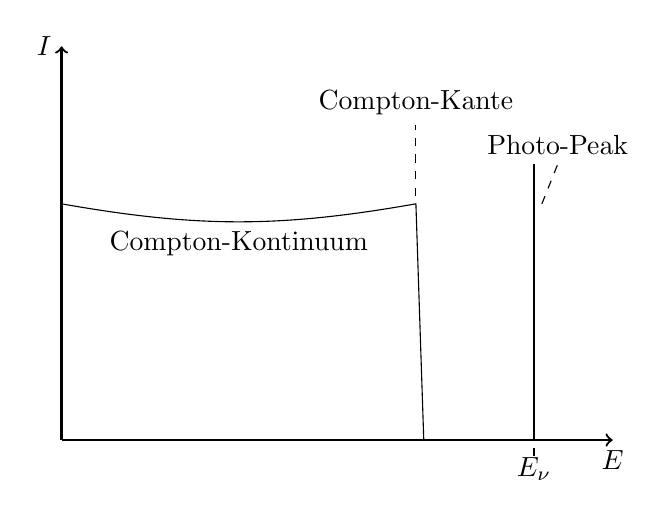
\begin{tikzpicture}
        \draw[thick,->]
        (0,0) -- (0,5) node[left] {$I$}
        ;
        \draw[thick,->]
        (0,0) -- (7,0) node[below] {$E$}
        ;
        \draw
        (6,0) -- (6,3.5)
        ;
        \draw
        (6,-.2) -- (6,-.1) node[below] {$E_\nu$}
        ;
        \draw[bend right=10]
        (0,3) to node[below] {Compton-Kontinuum} (4.5,3) -- (4.6,0)
        ;
        \draw[dashed]
        (4.5,3.1) -- (4.5,4) node[above] {Compton-Kante}
        ;
        \draw[dashed]
        (6.1,3) -- (6.3,3.5) node[above] {Photo-Peak}
        ;
    \end{tikzpicture}
    \caption{%
        Idealisiertes Spektrum der bei Einstrahlung von monochromatischer
        $\gamma$-Strahlung an den Szintillator übertragenen Energie
    }
    \label{fig:Compton}
\end{figure}

\section{Instrumente}

\subsection{Szintillator}

Zur Detektion von $\gamma$-Quanten verwendet man einen Kristall, zum Beispiel
Natriumiodid. Trifft nun ein $\gamma$ auf ein Elektron, wird es angeregt. Bei
der Abregung, die über Zwischenniveaus stattfindet, werden Photonen abgegeben,
welche von einem Photomultiplier eingefangen werden können. Die Intensität des
Lichtblitzes ist dabei proportional zur Energie des ursprünglichen
$\gamma$-Quants.

\subsection{Photomultiplier (PM)}

Will man ein schwaches optisches Signal in eine messbares elektrisches Signal
umwandeln, benötigt man einen Photomultiplier. Ein möglicher Aufbau ist in
Abbildung~\ref{fig:PM} zu sehen. Zwischen Photokathode und Anode liegt eine
Spannung an, die von Dynode zu Dynode abfällt.

Trifft ein Photon auf die Photokathode, löst es, wenn seine Energie die
Austrittsarbeit übersteigt, ein Elektron aus dieser heraus. Durch die angelegte
Spannung wird das Elektron beschleunigt und zum Beispiel durch ein Elektrisches
Feld so abgelenkt, dass es auf die erste Dynode trifft. Hier löst es weitere
Elektronen aus, die zur nächsten Dynode beschleunigt werden. Der Prozess geht
so weiter, bis zum Schluss die Lawinenelektronen auf die Anode treffen und dort
ein messbares elektronisches Signal ergeben.

Da die Anzahl der ausgelösten Elektronen proportional zur Intensität der
eintreffenden Strahlung ist, und da der Photomultiplier linear verstärkt. Ist
das Ausgangssignal proportional zur einfallenden Intensität. Wird ein
Szintillatorsignal verstärkt, ist die Amplitude also proportional zur Energie
der $\gamma$-Strahlung.

An der Anode liegt meisten Sättigung vor. Dies sorgt dafür, dass die Amplitude
des Signals keine Aussage mehr über die Energie machen kann, aber durch eine
Anstiegszeit von wenigen \si{\nano\second} eine hohe Zeitgenauigkeit erreicht
wird. Wegen des schnellen Anstiegs wird das Ausgangssignal daher auch
\emph{Fast}-Signal genannt.

Greift man das Signal an einer Dynode, an der noch keine Sättigung herrscht ab,
ist eine Aussage über die Energie des verursachenden Photons möglich. Die
Anstiegszeit ist jedoch deutlich größer. Daher heißt dieses Signal auch
\emph{Slow}-Signal.

\begin{figure}[htbp]
    \centering
    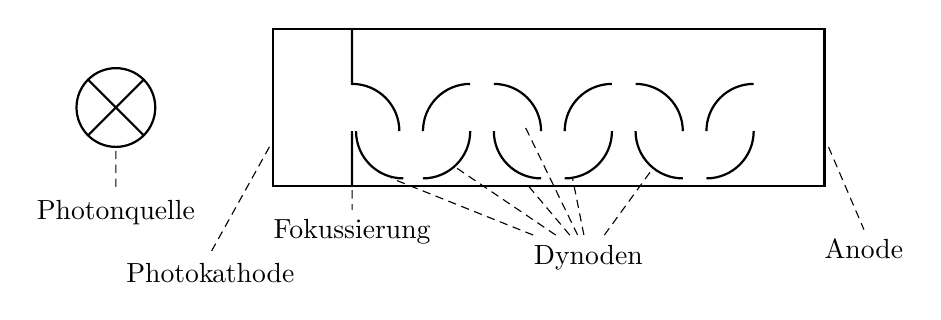
\begin{tikzpicture}
        % Röhre
        \draw[thick] (2,-1) rectangle (9,1);
        % Photonquelle
        \draw[thick]
        (0,0) circle (.5)
        (225:.5) -- (45:.5)
        (135:.5) -- (-45:.5)
        ;
        % Photokathode und Anode
        \draw[thick]
        (2,1) -- (2,-1)
        (9,1) -- (9,-1)
        ;
        % Dynoden
        \draw[thick]
        (3,-.3) -- (3,-1)
        (3,1) -- (3,.3) arc (90:0:.6cm)
        (3.05,-.3) arc (180:270:.6cm)
        (3.9,-.9) arc (270:360:.6cm)
        (3.9,-.3) arc (180:90:.6cm)
        (4.8,.3) arc (90:0:.6cm)
        (4.8,-.3) arc (180:270:.6cm)
        (5.7,-.9) arc (270:360:.6cm)
        (5.7,-.3) arc (180:90:.6cm)
        (6.6,.3) arc (90:0:.6cm)
        (6.6,-.3) arc (180:270:.6cm)
        (7.5,-.9) arc (270:360:.6cm)
        (7.5,-.3) arc (180:90:.6cm)
        ;
        % Beschriftungen PQ, PK, A und Fokussierung
        \draw[densely dashed]
        (0,-.55) -- (0,-1.05) node[below] {Photonquelle}
        (1.95,-.5) -- (1.2,-1.85) node[below] {Photokathode}
        (3,-1.05) -- (3,-1.3) node[below] {Fokussierung}
        (9.05,-.5) -- (9.5,-1.55) node[below] {Anode}
        ;
        % Beschriftung Dynoden
        \node (D) at (6,-1.9) {Dynoden};
        \draw[densely dashed]
        (D) -- (3.5,-.9)
        (D) -- (4.3,-.75)
        (D) -- (5.2,-.95)
        (D) -- (5.2,-.25)
        (D) -- (5.8,-.9)
        (D) -- (6.8,-.8)
        ;
    \end{tikzpicture}
    \caption{%
        Möglicher Aufbau eines Photomultipliers
    }
    \label{fig:PM}
\end{figure}

\subsection{Splitter}

Will man ein Signal ohne es zu verformen aufteilen, benötigt man einen
Splitter. Dieser ist meist durch einige Widerstände realisiert. Steckt man nur
drei Kabel aneinander, werden die Signale unter Umständen unterschiedlich
aufgeteilt. Zudem treten Reflektionen auftreten, die das Signal verfälschen
können.

\subsection{Verstärker}

Der Verstärker/Operationsverstärker (engl. \emph{amplifier}) ist ein
elektrisches Bauteil, welches die Aufgabe hat ein eingehendes Signal zu
verstärken. Diese Verstärkung ist nur für einen Eingangs-Amplituden-Bereich und
einen Verstärkungsbereich linear. Da bei vielen Anwendungen Linearität
gewährleistet sein muss, werden meist Vor- und Hauptverstärker verwendet.

\subsection{Constant Fraction Diskriminator (CFD)}

Ein Diskriminator ist ein Gerät, welches nur anspricht, wenn ein eintreffendes
Signal stärker ist, als ein bestimmter Grenzwert (engl. \emph{threshold}).
Trifft ein solches Signal ein, gibt der Diskriminator ein Standardsignal, zum
Beispiel ein Rechtecksignal aus.

Eine Anwendung des Diskriminators ist das Triggern: Trifft ein Signal ein, wird
ein neues, standardisiertes abgegeben. So ist zum Beispiel der zeitliche
Abstand zwischen zwei eintreffenden Signalen zu messen. Wann genau der
Diskriminator triggert, kommt auf die Art an.

Der CFD triggert, wenn ein bestimmter Anteil der Maximalamplitude erreicht
wird.Dazu wird das einkommende Signal gesplittet, ein Teil wird zeitlich
verzögert, der andere invertiert und um einen Faktor $k$ gedämpft. Anschließend
werden beide Signale wieder addiert. Ein vorher rein positives Signal erhält so
eine Nullstelle, welche durch $k$ bestimmt wird und den Triggerpunkt definiert.

\subsection{Einkanalanalysator (SCA)}

Der SCA (engl. \emph{single channel analyser}) ist ein elektrisches Bauteil,
welches wie ein Diskriminator eine Untergrenze hat, unter der Signale blockiert
werden. Zusätzlich besitzt er eine Obergrenze, sodass nur Signale mit einer
Amplitude innerhalb eines bestimmten Bereiches (engl. \emph{window}) betrachtet
werden. Er gibt ein logisches Signal ab, wenn die Amplitude eines einkommendes
Signals aus diesem Bereich wieder unterhalb die Untergrenze fällt.

\subsection{Vielkanalanalysator (MCA)}

Der Vielkanalanalysator (engl. \emph{multi channel analyser}) sortiert
einkommende Signale nach Amplitude. Trifft ein Signal mit einer bestimmten
Amplitude ein, setzt er einen Zähler in einem bestimmten Kanal hoch. Dadurch
zählt der MCA wie häufig die verschiedenen Amplituden auftauchen. Es entsteht
eine Art Histogramm.

\subsection{Koinzidenzeinheit}

Eine Koinzidenzeinheit gibt ein logisches Signal aus, wenn zwei oder mehr
eingehende Signale zeitlich überlappen. Dies kann zum Beispiel realisiert
werden, indem die Amplituden der Signale addiert werden und an einen SCA
übergeben werden, welcher so eingestellt ist, dass er nur anspricht, wenn ein
Signal mit einer Amplitude einkommt, welches der Summe aller eintreffenden
Signale entspricht.

\subsection{Zeit-Impulshöhe-Konverter (TAC)}

Wie der Name schon sagt, konvertiert ein TAC (engl. \emph{time amplitude
converter}) ein Zeitabstand in ein Signal mit einer zu dieser Zeitdifferenz
proportionalen Amplitude. Dies wird erreicht, indem bei einem Startsignal ein
Kondensator mit einem konstanten Strom geladen wird. Bei einem Stopsignal wird
dieser Kondensator über einen Widerstand entladen. Die Spannung zwischen den
Kondensatorplatten ist proportional zur Zeitdifferenz und die Amplitude
proportional zur Spannung. Somit ist die Amplitude proportional zeitlichen
Abstand der Eingangssignale.

%%%%%%%%%%%%%%%%%%%%%%%%%%%%%%%%%%%%%%%%%%%%%%%%%%%%%%%%%%%%%%%%%%%%%%%%%%%%%%%
%                                Durchführung                                %
%%%%%%%%%%%%%%%%%%%%%%%%%%%%%%%%%%%%%%%%%%%%%%%%%%%%%%%%%%%%%%%%%%%%%%%%%%%%%%%

\chapter{Durchführung}

\section{Slow-Koinzidenzkreis einstellen}

Bei der Durchführung am ersten Tag sind wir an einigen Stellen nicht exakt in
der Reihenfolge der Anleitung vorgegangen. Zur besseren Übersicht haben wir
hier die Reihenfolge etwas sortiert. Dabei haben wir auch die Kalibrierung des
linken und rechten Detektors zusammengefasst, um vor allem bei den Abbildungen
einen direkten Vergleich bieten zu können.

\subsection{Slow-Pulse des Photomultipliers kontrollieren}

Wir betrachten das Slow-Signal des linken Photomultipliers auf dem Oszilloskop
wie in Abbildung~\ref{fig:aufbau:slow} gezeigt. Das Oszillogramm ist in
Abbildung~\ref{fig:slow_signal}, links/* Bild 16:26*/. Dann schauen wir uns das
Slow-Signal des rechten PM auf dem Oszilloskop an, siehe
Abbildung~\ref{fig:slow_signal}, rechts.

\begin{figure}[htbp]
    \centering
    \begin{tikzpicture}
        \node[device] (na) {$^{22}\mathrm{Na}$};
        \node[device] (pm) [right=of na] {Photomultiplier};
        \node[monitor] (oszi) [right=of pm] {Oszilloskop};

        % Teilchenaustausch
        \begin{scope}[->, dotted, thick]
            \draw (na) -- (pm);
        \end{scope}

        % Analogsignal
        \begin{scope}[->]
            \draw (pm) -- (oszi);
        \end{scope}

        % Digitalsignal
        \begin{scope}[->, dashdotted]
        \end{scope}
    \end{tikzpicture}
    \caption{%
        Aufbau zum Betrachten des Slow-Signals. Die gepunktete Linie stellt
        Teilchenaustausch (Elektronen, $\gammaup$-Strahlung, …) dar. Die
        durchgezogene Linie ist ein analoges elektrisches Signal. Messgeräte,
        die etwas anzeigen, markieren wir durch die abgerundeten Ecken.
    }
    \label{fig:aufbau:slow}
\end{figure}

\begin{figure}[htbp]
    \centering
    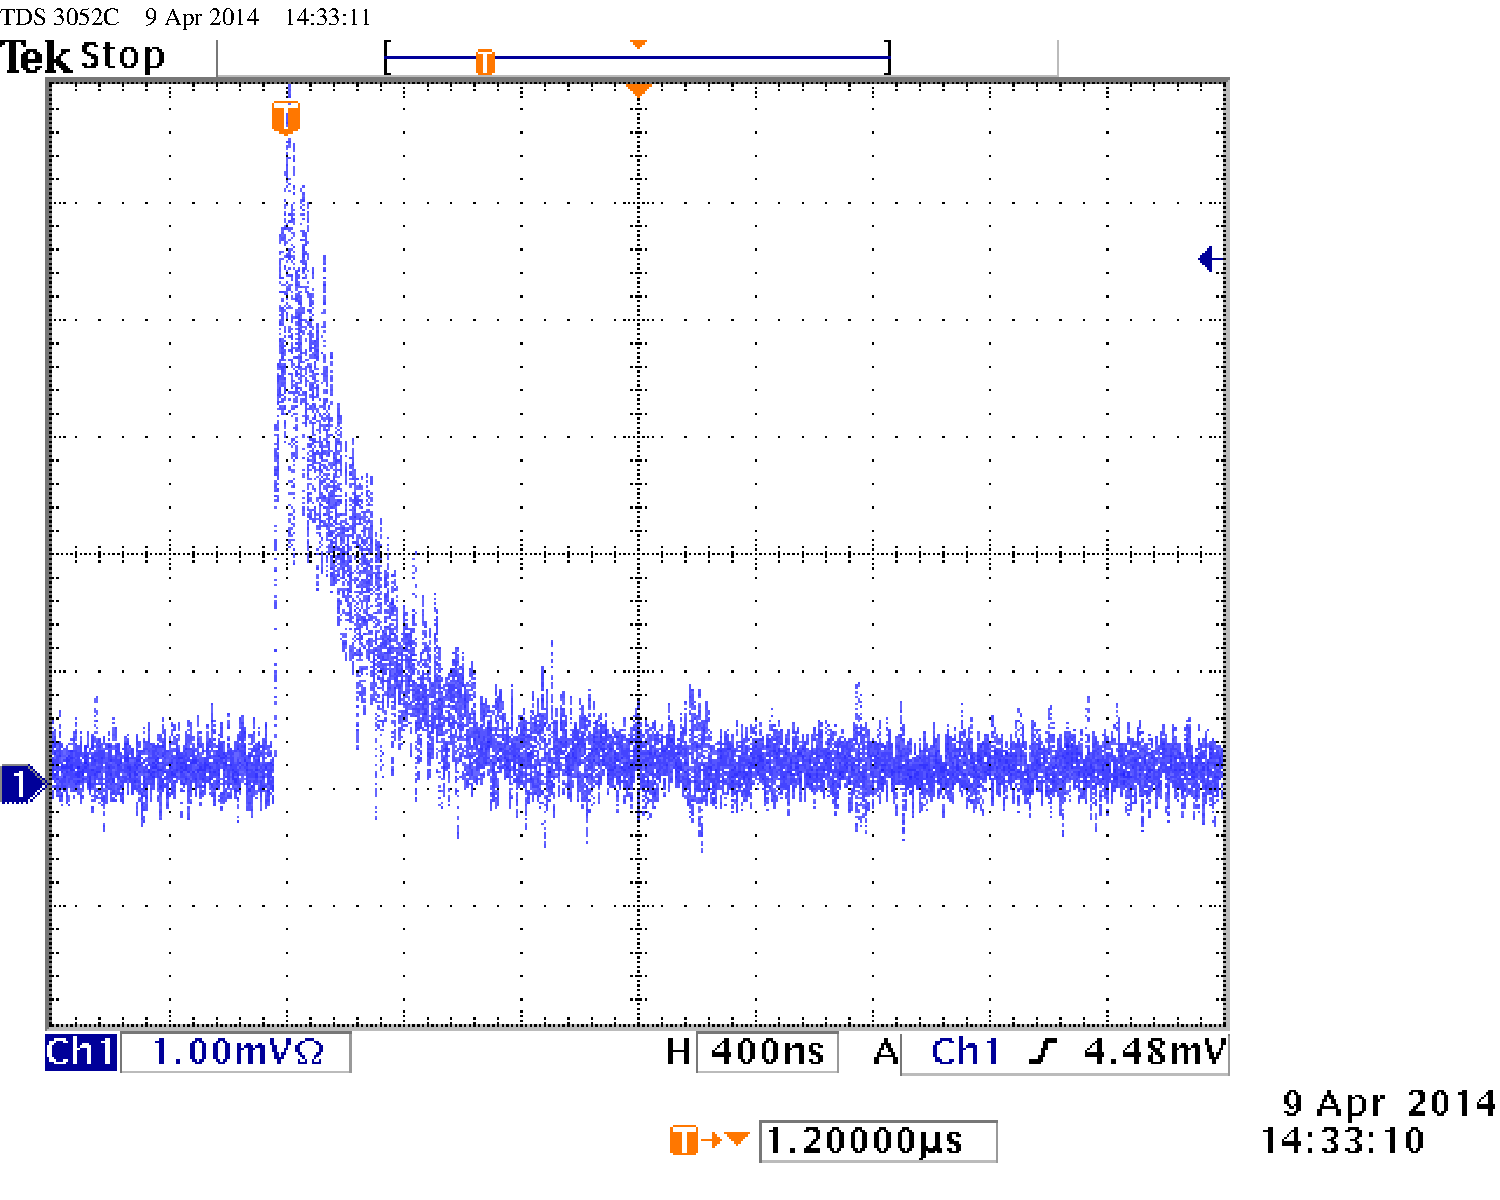
\includegraphics[width=0.49\linewidth]{../Daten/2014-04-09_14-33-east.pdf}
    \hfill
    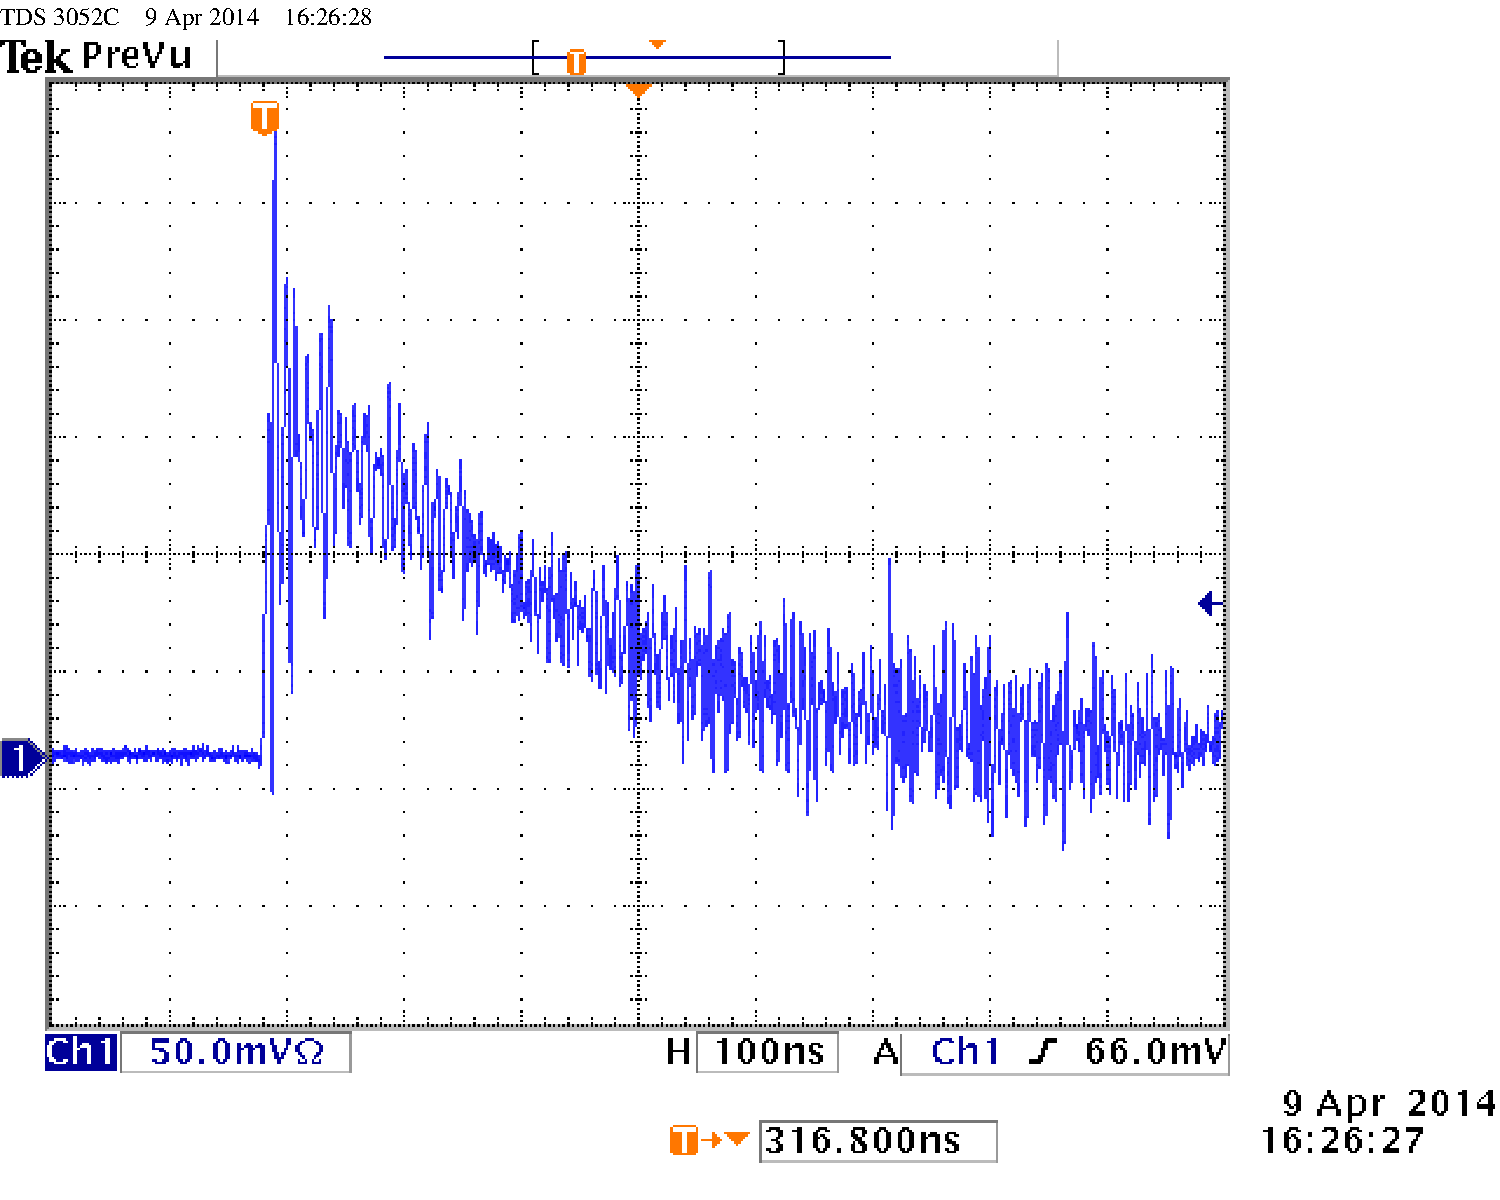
\includegraphics[width=0.49\linewidth]{../Daten/2014-04-09_16-26-east.pdf}
    \caption{%
        Slow-Signale von linkem und rechten Detektor.
    }
    \label{fig:slow_signal}
\end{figure}

An beiden Signalen ist der exponentielle Abfall des Signals zu erkennen, das
durch der Abklingzeit des Szintillators erzeugt wird.

Danach betrachten wir das Signal nach dem Vorverstärker des linken /* Bildzeit
14:58 */ und rechten /* Bildzeit 16:39 */ Detektors, siehe
Abbildung~\ref{fig:slow_pre_amp}. Der Aufbau ist in
Abbildung~\ref{fig:aufbau:slow_pre} dargestellt.

\begin{figure}[htbp]
    \centering
    \begin{tikzpicture}
        \node[device] (na) {$^{22}\mathrm{Na}$};
        \node[device] (pm) [right=of na] {Photomultiplier};
        \node[device] (preamp) [right=of pm] {Vorverstärker};
        \node[monitor] (oszi) [right=of preamp] {Oszilloskop};

        % Teilchenaustausch
        \begin{scope}[->, dotted, thick]
            \draw (na) -- (pm);
        \end{scope}

        % Analogsignal
        \begin{scope}[->]
            \draw (pm) -- (preamp);
            \draw (preamp) -- (oszi);
        \end{scope}

        % Digitalsignal
        \begin{scope}[->, dashdotted]
        \end{scope}
    \end{tikzpicture}
    \caption{%
        Aufbau zum Betrachten des Slow-Signals nach dem Vorverstärker.
    }
    \label{fig:aufbau:slow_pre}
\end{figure}

\begin{figure}[htbp]
    \centering
    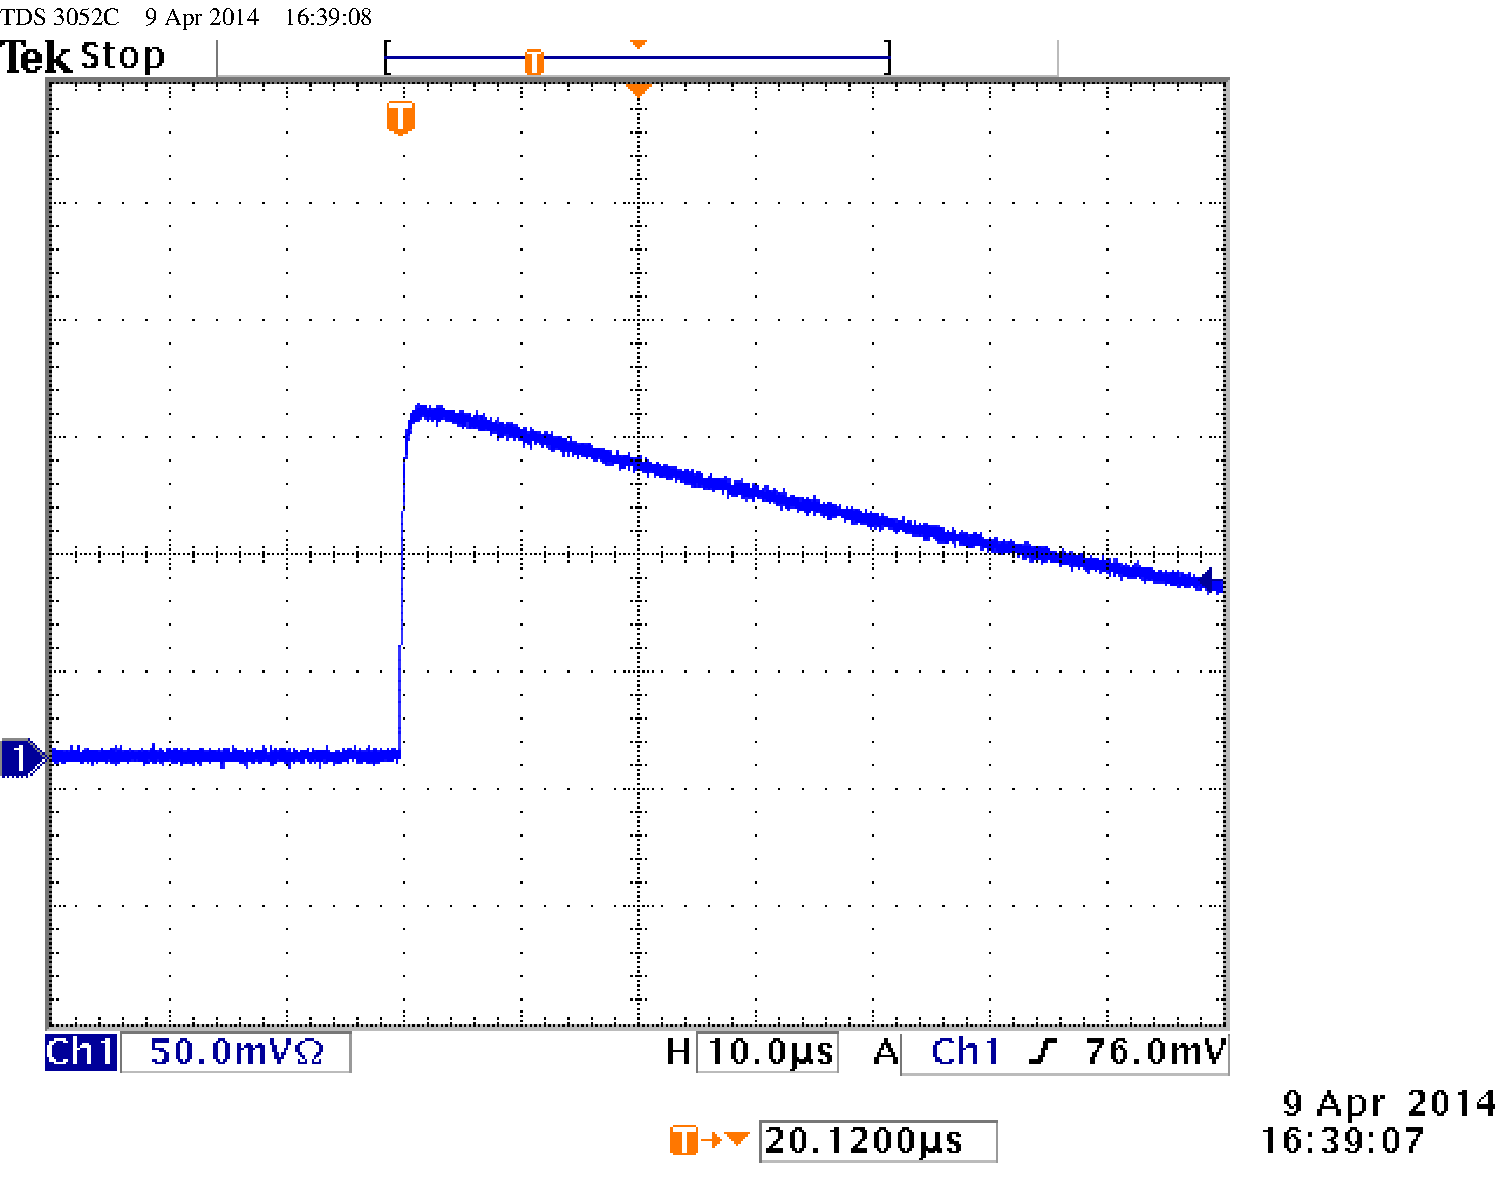
\includegraphics[width=0.49\linewidth]{../Daten/2014-04-09_16-39-east.pdf}
    \hfill
    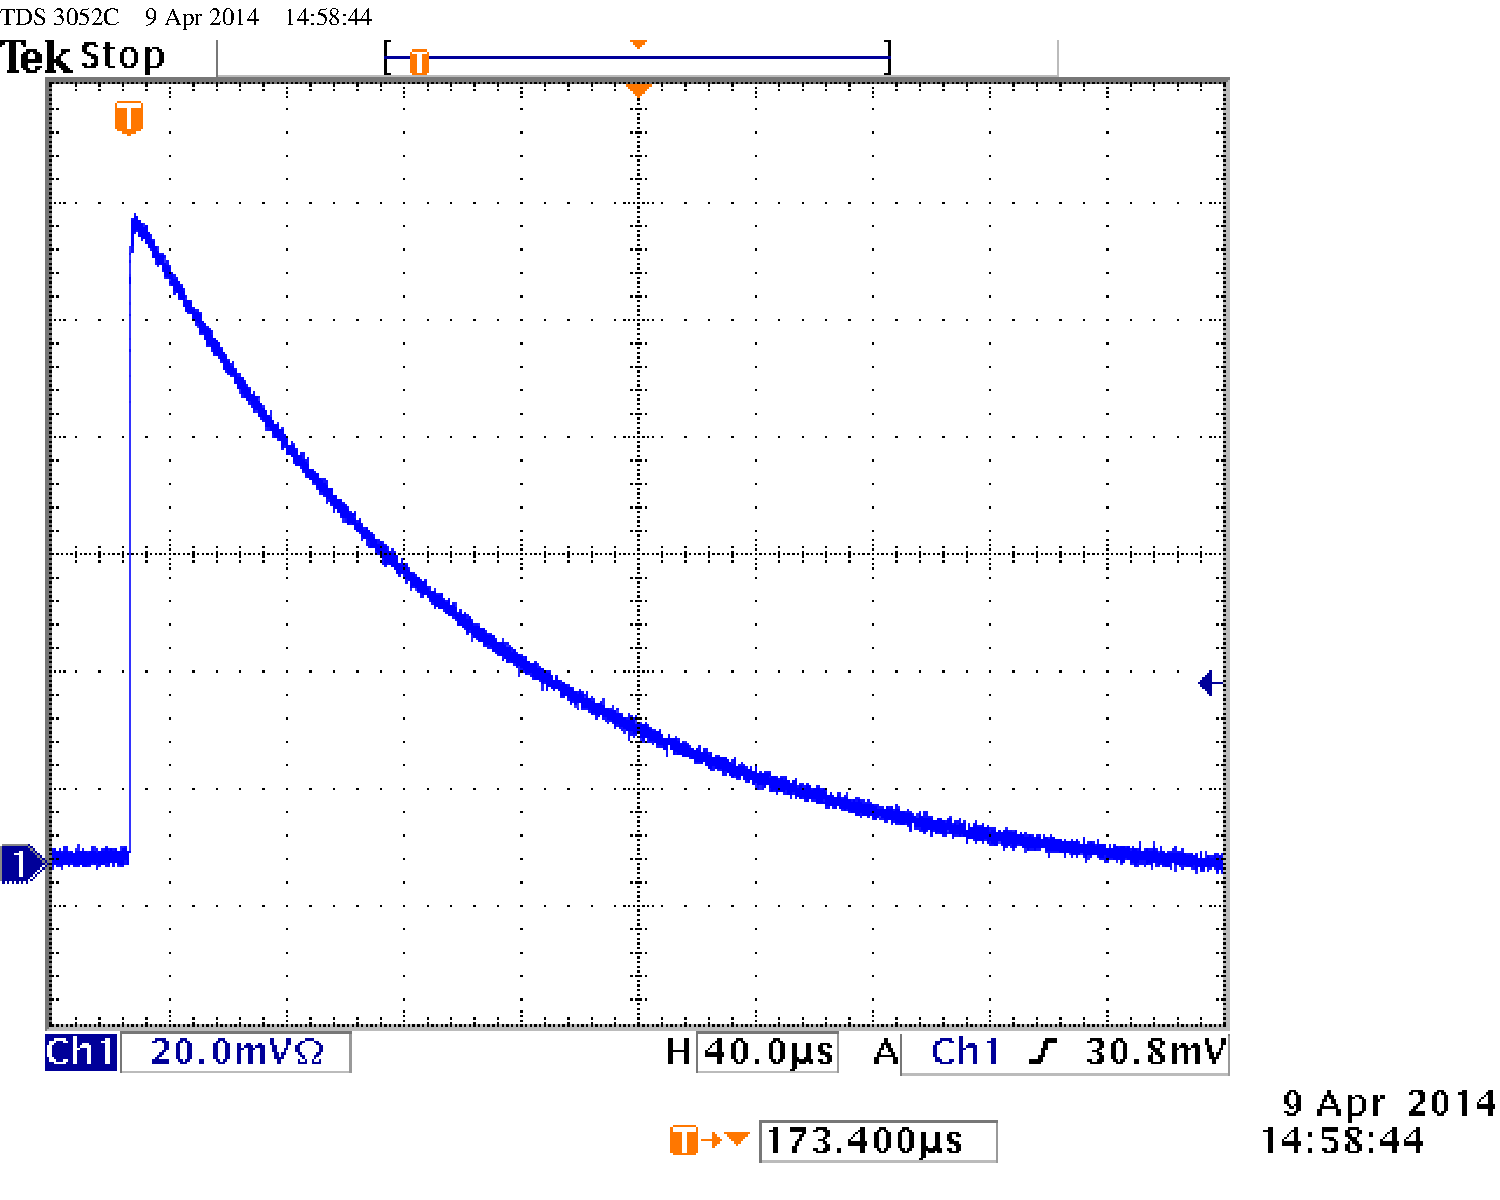
\includegraphics[width=0.49\linewidth]{../Daten/2014-04-09_14-58-east.pdf}
    \caption{%
        Slow-Signal nach dem Vorverstärker für den linken und rechten Detektor.
    }
    \label{fig:slow_pre_amp}
\end{figure}

Der Vorverstärker zieht die Pulse, die wir an der Dynode abnehmen, stark in die
Länge. Dies wird erst im nächsten Schritt wieder korrigiert. Dafür erhalten wir
etwas Verstärkung.

Wir schließen den Hauptverstärker nach dem Vorverstärker an, siehe
Abbildung~\ref{fig:aufbau:slow_amp}. Dessen Ausgang betrachten wir auf dem
Oszilloskop/* Bildzeit links 15:03, rechts 16:41 */, siehe
Abbildung~\ref{fig:slow_amp}.

\begin{figure}[htbp]
    \centering
    \begin{tikzpicture}
        \node[device] (na) {$^{22}\mathrm{Na}$};
        \node[device] (pm) [right=of na] {Photomultiplier};
        \node[device] (preamp) [right=of pm] {Vorverstärker};
        \node[device] (amp) [right=of preamp] {Verstärker};
        \node[monitor] (oszi) [right=of amp] {Oszilloskop};

        % Teilchenaustausch
        \begin{scope}[->, dotted, thick]
            \draw (na) -- (pm);
        \end{scope}

        % Analogsignal
        \begin{scope}[->]
            \draw (pm) -- (preamp);
            \draw (preamp) -- (amp);
            \draw (amp) -- (oszi);
        \end{scope}

        % Digitalsignal
        \begin{scope}[->, dashdotted]
        \end{scope}
    \end{tikzpicture}
    \caption{%
        Aufbau zum Betrachten des Slow-Signals nach dem Hauptverstärker
    }
    \label{fig:aufbau:slow_amp}
\end{figure}

\begin{figure}[htbp]
    \centering
    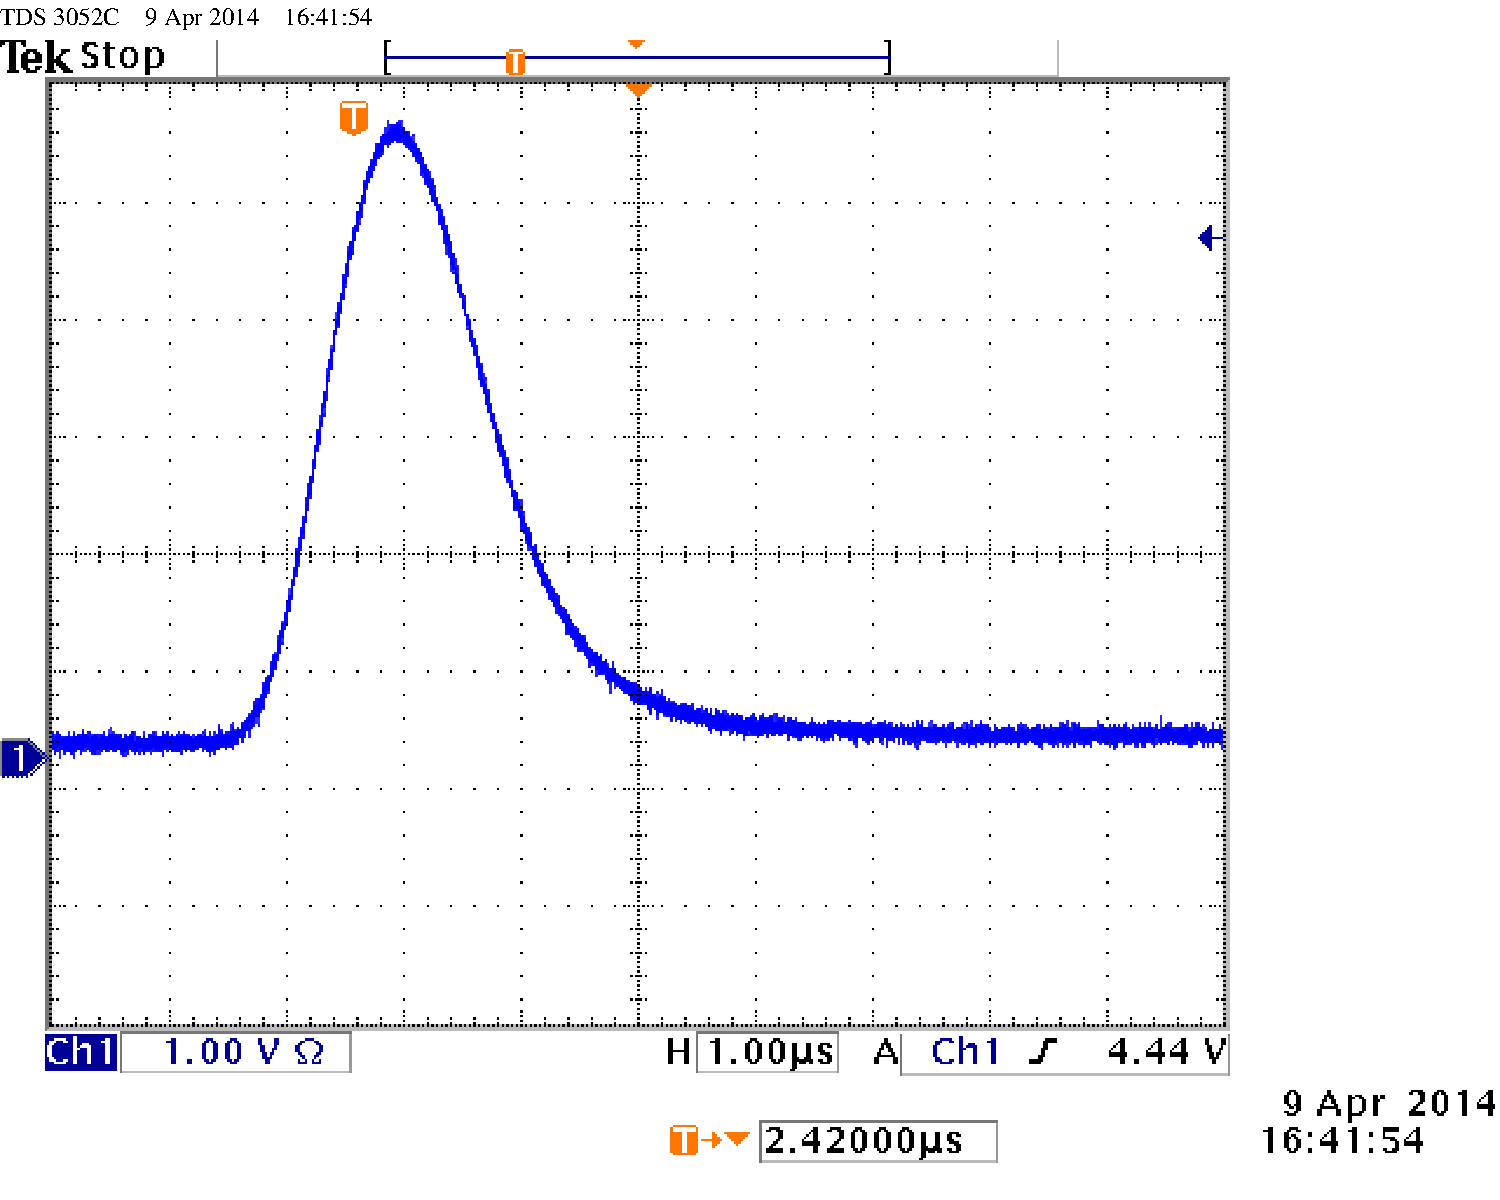
\includegraphics[width=0.49\linewidth]{../Daten/2014-04-09_16-41-east.pdf}
    \hfill
    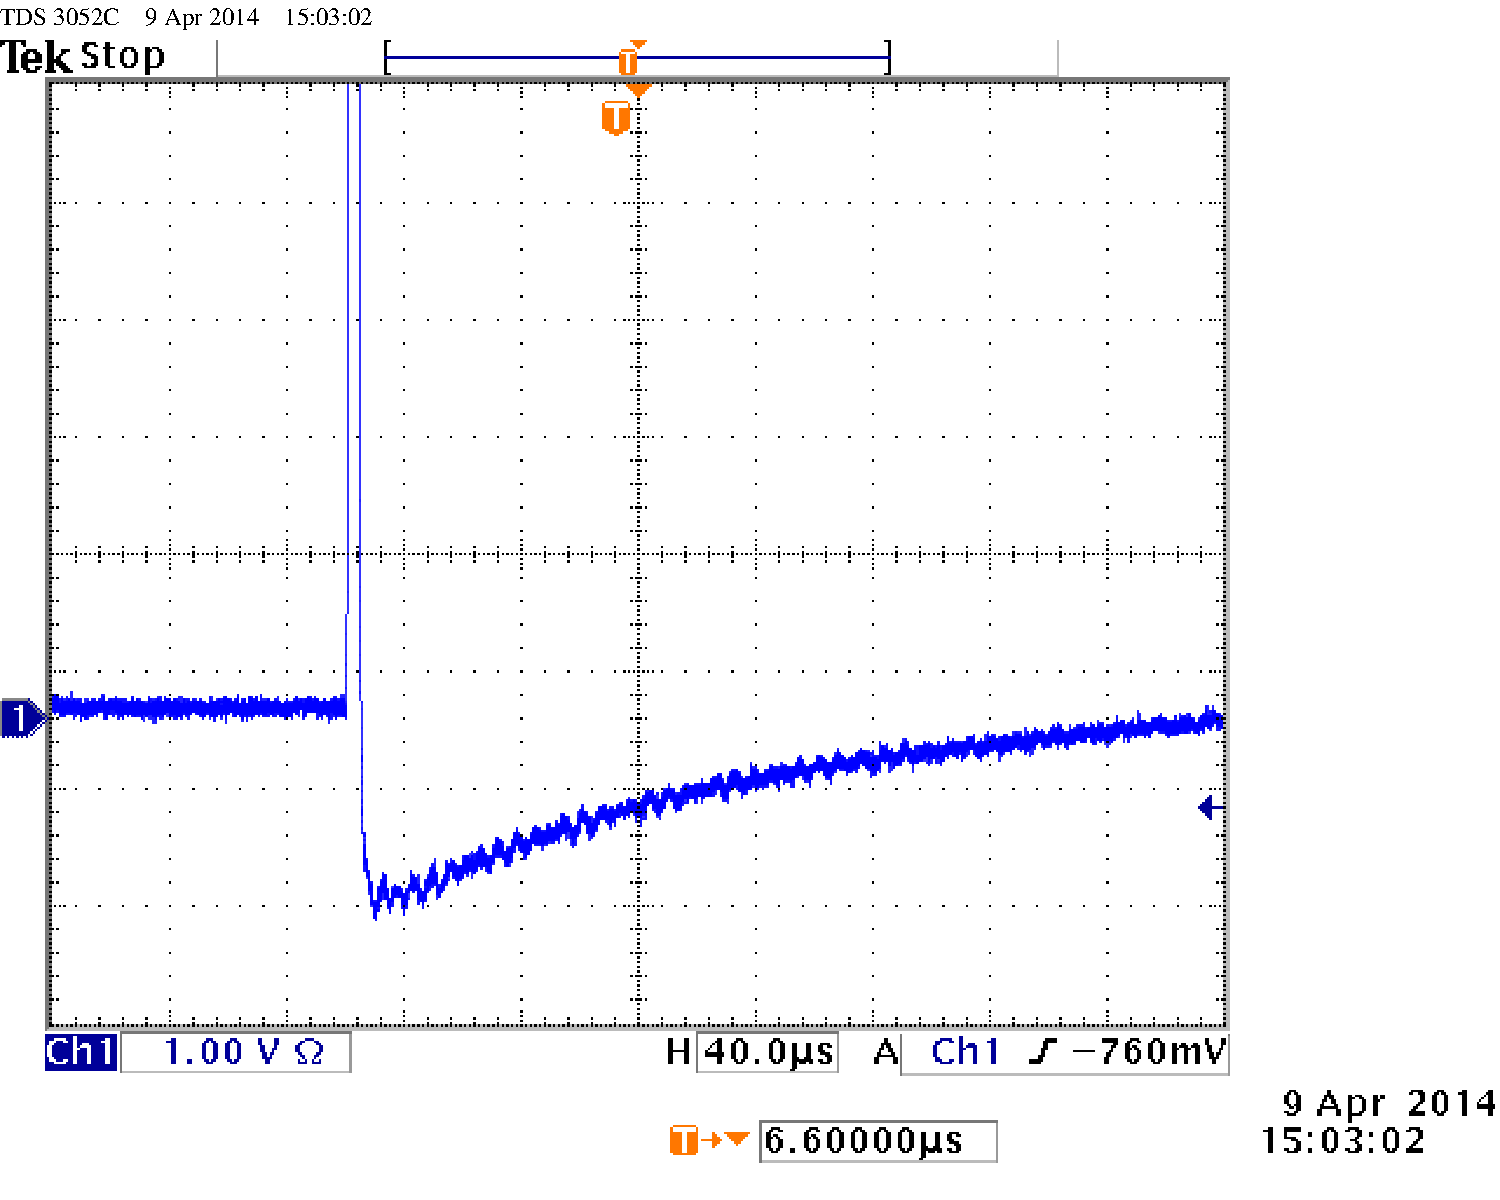
\includegraphics[width=0.49\linewidth]{../Daten/2014-04-09_15-03-east.pdf}
    \caption{%
        Slow-Signal nach dem Verstärker
    }
    \label{fig:slow_amp}
\end{figure}

An der Zeiteinteilung der Bildschirmfotos ist zu erkennen, dass die Pulse jetzt
wieder sehr kurz sind. Der Hauptverstärker kürzt die Pulse, allerdings werden
sie teilweise ins Negative gezogen, wie beim rechten Zweig zu sehen ist.

\subsection{Triggerung mit dem SCA}

Wir schließen den Ausgang des linken Hauptverstärkers an den Splitter an. Der
eine Ausgang geht an das SCA. Der Andere an den Delay-Verstärker. Die Ausgänge
beider Geräte betrachten wir mit dem Oszilloskop, siehe
Abbildung~\ref{fig:aufbau:sca_trigger}. Nun versuchen wir, die Verzögerung so
einzustellen, dass das digitale Signal des SCA den Puls vom Verstärker
umschließt. Dies gelingt uns allerdings nicht, weil das digitale Signal zu kurz
ist. Dass das digitale Signal zu kurz ist, ist auch in Abbildung~\ref{fig:511}
zu erkennen.

\begin{figure}[htbp]
    \centering
    \begin{tikzpicture}
        \node[device] (na) {$^{22}\mathrm{Na}$};
        \node[device] (pm) [right=of na] {Photomultiplier};
        \node[device] (amp) [right=of pm] {Verstärker};
        \node[device] (split) [right=of amp] {Splitter};
        \node[device] (delay) [right=of split] {Verzögerung};
        \node[device] (sca) [below=of split] {SCA};
        \node[monitor] (oszi) [below=of delay] {Oszilloskop};

        % Teilchenaustausch
        \begin{scope}[->, dotted, thick]
            \draw (na) -- (pm);
        \end{scope}

        % Analogsignal
        \begin{scope}[->]
            \draw (pm) -- (amp);
            \draw (amp) -- (split);
            \draw (split) -- (delay);
            \draw (split) -- (sca);
            \draw (delay) -- (oszi);
        \end{scope}

        % Digitalsignal
        \begin{scope}[->, dashdotted]
            \draw (sca) -- (oszi);
        \end{scope}
    \end{tikzpicture}
    \caption{%
        Aufbau zur Triggerung mit dem SCA. Um Platz zu sparen, fassen wir ab
        hier den Vorverstärker und den Hauptverstärker zu einem Bauteil
        zusammen. Die gestrichpunktete Linie stellt ein digitales Signal dar.
        Das Oszilloskop wird mit dem digitalen Signal getriggert.
    }
    \label{fig:aufbau:sca_trigger}
\end{figure}

Wir regeln den Verstärker auf Faktor 20 herunter. Im Nachleuchten auf dem
Oszilloskop ist eine Amplitude zu erkennen, die besonders häufig vorkommt. Davon
haben wir ein Bild so gespeichert, dass diese Linie auch besonders stark
repräsentiert ist/* Bildzeit 15:20 */, siehe Abbildung~\ref{fig:511}. Diese
Linie wird die \SI{511}{\kilo\electronvolt}-Linie sein.

\begin{figure}[htbp]
    \centering
    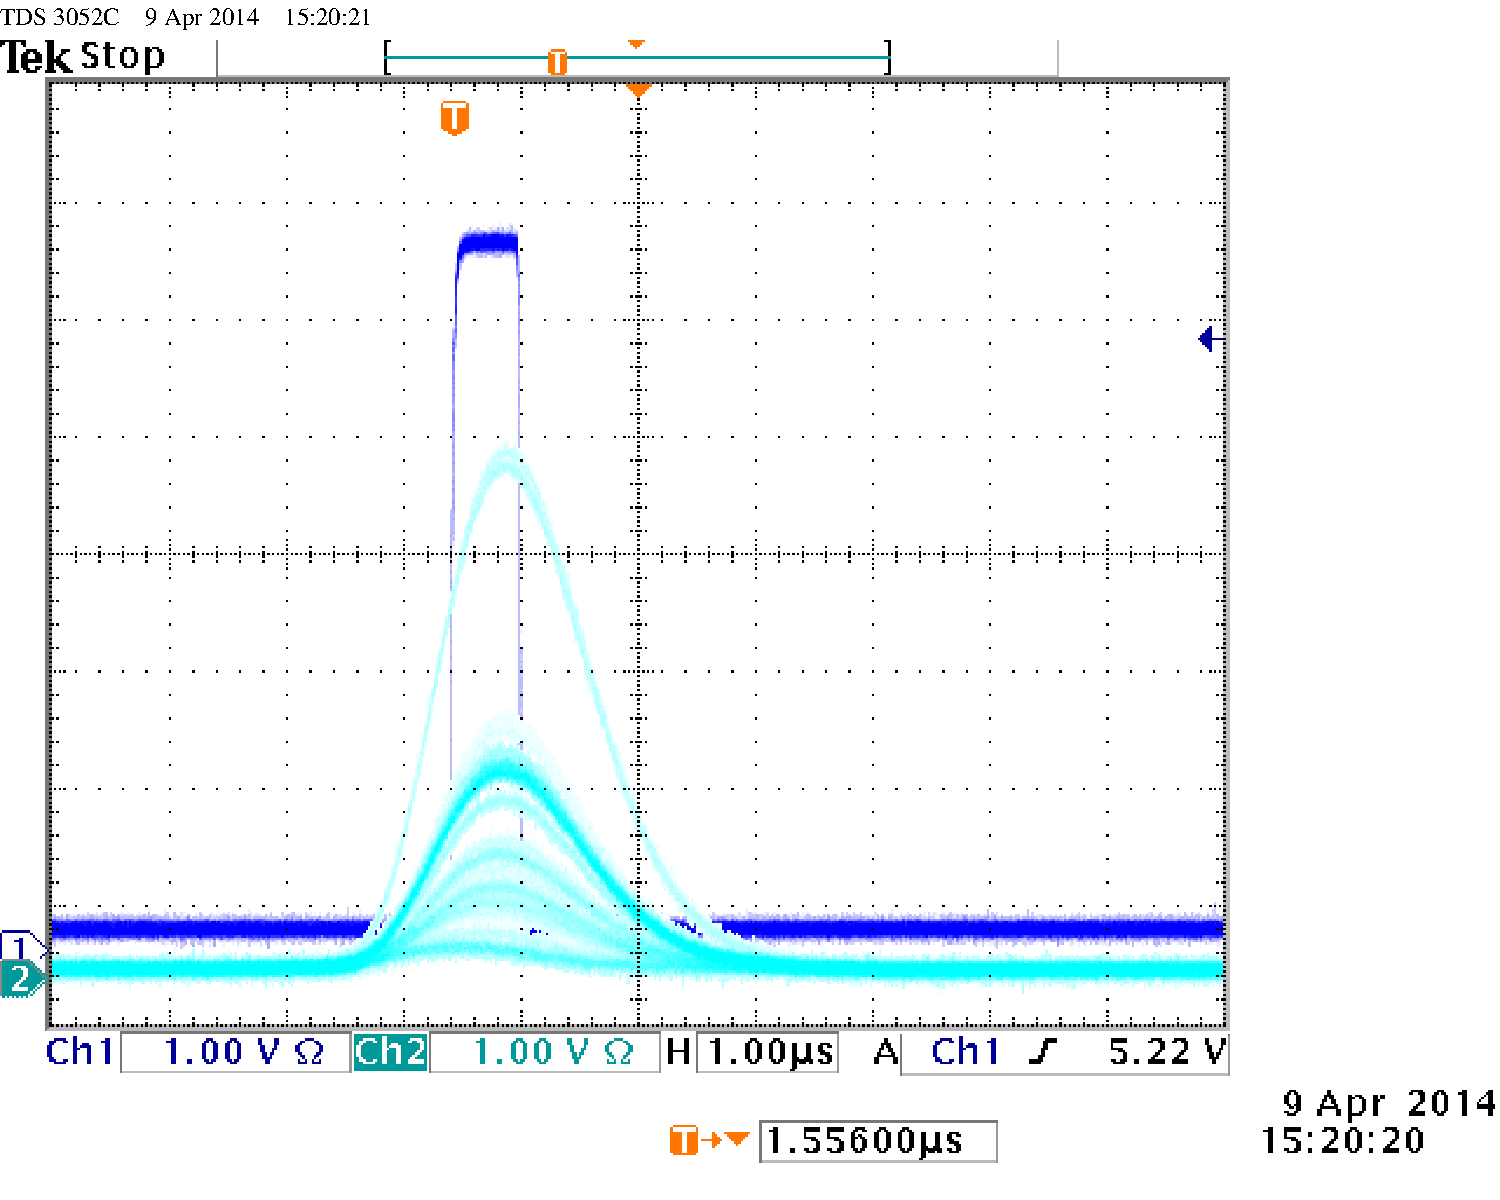
\includegraphics[width=0.49\linewidth]{../Daten/2014-04-09_15-20-east.pdf}
    \caption{%
        Besonders häufig vorkommende Linie im Signal des Verstärkers.
    }
    \label{fig:511}
\end{figure}

Zwischen SCA und Oszilloskop schalten wir noch den GDG
(Abbildung~\ref{fig:aufbau:sca_gdg}). Am SCA stellen wir die Verzögerung auf 0.
Das GDG justieren wir so, dass das digitale Signal die Pulse umschließt/*
Bildzeit 15:27, scheint aber nicht geklappt zu haben. */. Am linken Delay-Amp
stellen wir eine Verzögerung von \SI{3.25}{\micro\second} ein. Am GDG stellen
wir die Verzögerung aus. Am Rechten Delay haben wir eine Verzögerung von
\SI{3.5}{\micro\second} gewählt. Das Oszillogramm für den rechten Zweig
/* Bildzeit 16:47 */ haben wir in Abbildung~\ref{fig:sca_umschlossen}.

\begin{figure}[htbp]
    \centering
    \begin{tikzpicture}
        \node[device] (na) {$^{22}\mathrm{Na}$};
        \node[device] (pm) [above=of na] {Photomultiplier};
        \node[device] (amp) [right=of pm] {Verstärker};
        \node[device] (split) [right=of amp] {Splitter};
        \node[device] (delay) [right=of split] {Verzögerung};
        \node[device] (sca) [below=of split] {SCA};
        \node[device] (gdg) [right=of sca] {GDG};
        \node[monitor] (oszi) [right=of gdg] {Oszilloskop};

        % Teilchenaustausch
        \begin{scope}[->, dotted, thick]
            \draw (na) -- (pm);
        \end{scope}

        % Analogsignal
        \begin{scope}[->]
            \draw (pm) -- (amp);
            \draw (amp) -- (split);
            \draw (split) -- (delay);
            \draw (split) -- (sca);
            \draw (delay) -- (oszi);
        \end{scope}

        % Digitalsignal
        \begin{scope}[->, dashdotted]
            \draw (sca) -- (gdg);
            \draw (gdg) -- (oszi);
        \end{scope}
    \end{tikzpicture}
    \caption{%
        Aufbau zur Triggerung mit dem SCA und GDG.
    }
    \label{fig:aufbau:sca_gdg}
\end{figure}

\begin{figure}[htbp]
    \centering
    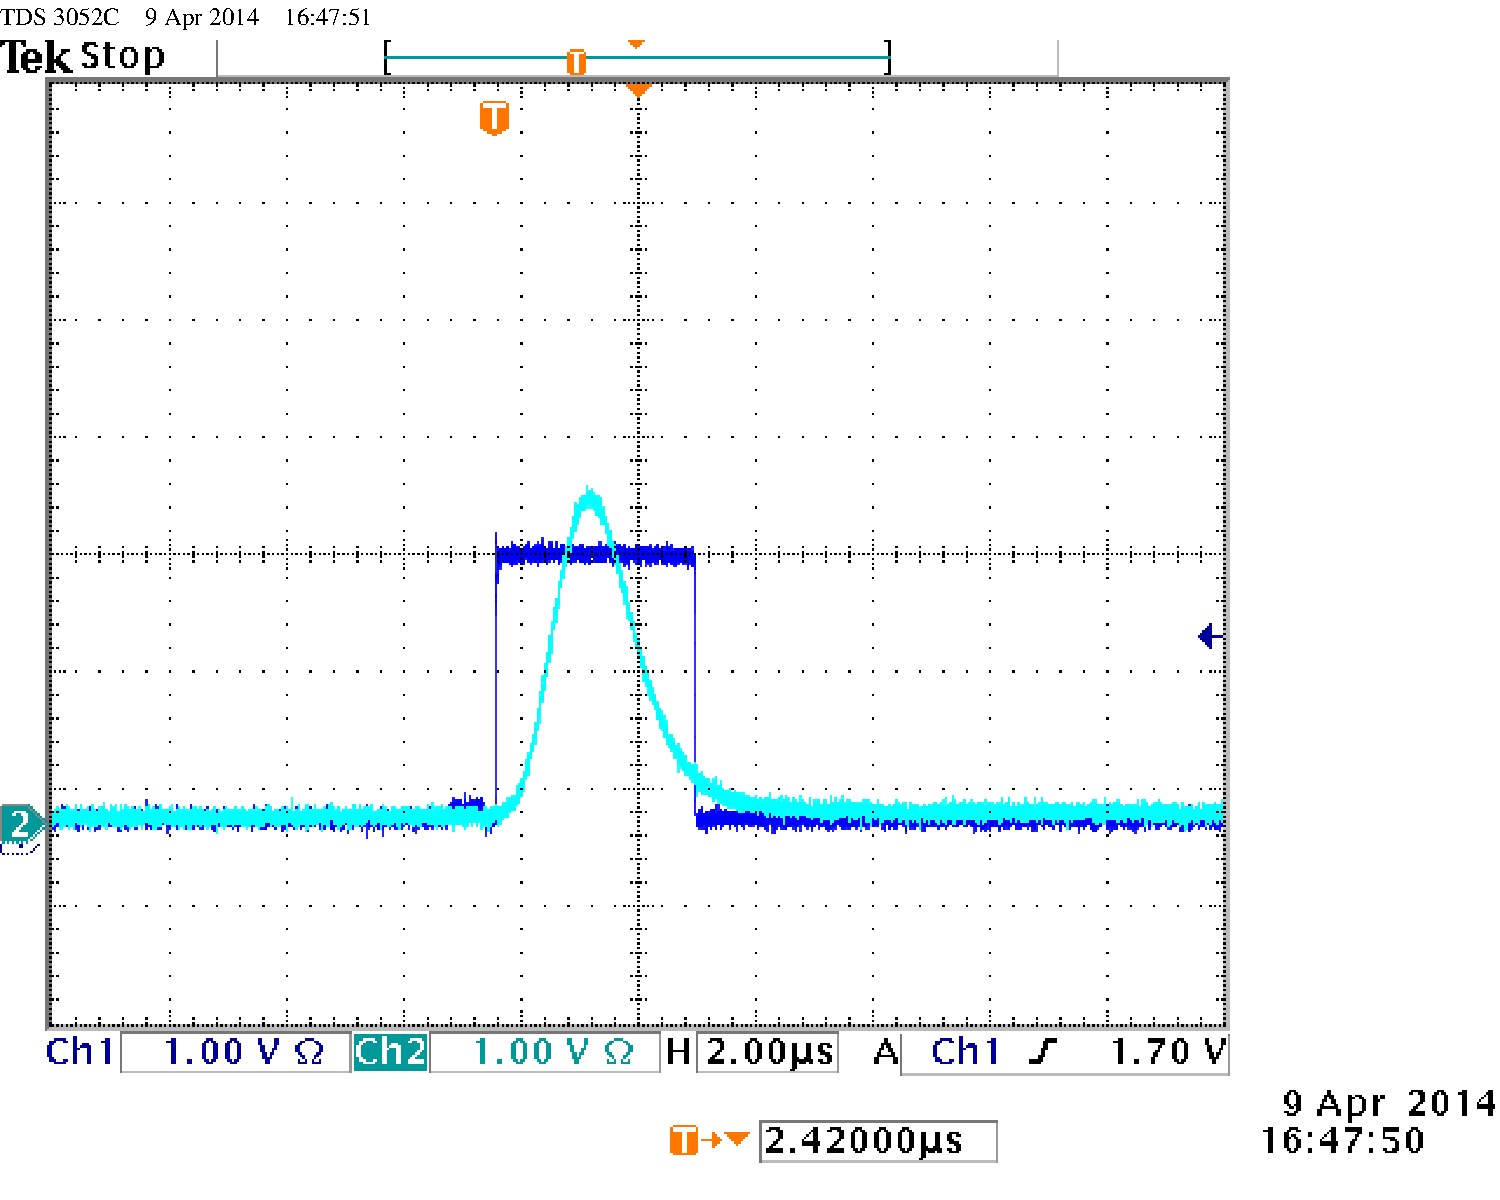
\includegraphics[width=0.49\linewidth]{../Daten/2014-04-09_16-47-east.pdf}
    \caption{%
        Slow-Signal des rechten Detektors nach dem Hauptverstärker im ersten
        Kanal. Das Signal aus dem rechten SCA im zweiten Kanal.
    }
    \label{fig:sca_umschlossen}
\end{figure}

Dort ist zu erkennen, dass mit dem verlängerten Logiksignal das analoge Signal
umschlossen werden kann.

Analog zum vorherigen Teil schließen wir den rechten Hauptverstärker an den
zweiten Splitter an. Die Ausgänge vom Splitter schließen wir an den anderen SCA
sowie an den einen GDG an.

\subsection{Energiespektrum für die ${}^{22}\text{Na}$-Quelle aufnehmen}

Nun ersetzen wir das Oszilloskop durch den MCA und betrachten das Spektrum,
siehe Abbildung~\ref{fig:aufbau:sca_gdg_mca}. Das
Fenster im SCA stellen wir auf die maximale Größe ein/* 001-Na.txt */, siehe
Abbildung~\ref{mca:001_004}.

\begin{figure}[htbp]
    \centering
    \begin{tikzpicture}
        \node[device] (na) {$^{22}\mathrm{Na}$};
        \node[device] (pm) [above=of na] {Photomultiplier};
        \node[device] (amp) [right=of pm] {Verstärker};
        \node[device] (split) [right=of amp] {Splitter};
        \node[device] (delay) [right=of split] {Verzögerung};
        \node[device] (sca) [below=of split] {SCA};
        \node[device] (gdg) [right=of sca] {GDG};
        \node[monitor] (mca) [right=of gdg] {MCA};

        % Teilchenaustausch
        \begin{scope}[->, dotted, thick]
            \draw (na) -- (pm);
        \end{scope}

        % Analogsignal
        \begin{scope}[->]
            \draw (pm) -- (amp);
            \draw (amp) -- (split);
            \draw (split) -- (delay);
            \draw (split) -- (sca);
            \draw (delay) -- (mca);
        \end{scope}

        % Digitalsignal
        \begin{scope}[->, dashdotted]
            \draw (sca) -- (gdg);
            \draw (gdg) -- (mca);
        \end{scope}
    \end{tikzpicture}
    \caption{%
        Aufbau zur Spektrumsaufnahme mit dem SCA und GDG. Das digitale Signal
        wird als Gate im MCA benutzt.
    }
    \label{fig:aufbau:sca_gdg_mca}
\end{figure}

\begin{figure}[htbp]
    \centering
    \begin{tikzpicture}
        \begin{axis}[width=0.45\linewidth, height=0.3\linewidth, xlabel=Kanal, ylabel=Ereignisse, axis lines=left]
            \addplot[black] table {../Daten/004-Na-rechts.txt};
        \end{axis}
    \end{tikzpicture}
    \hfill
    \begin{tikzpicture}
        \begin{axis}[width=0.45\linewidth, height=0.3\linewidth, xlabel=Kanal, ylabel=Ereignisse, axis lines=left]
            \addplot[black] table {../Daten/001-Na.txt};
        \end{axis}
    \end{tikzpicture}
    \caption{Spektrum der Na-Probe im rechten und linken Detektor}
    \label{mca:001_004}
\end{figure}

Damit das Spektrum den ganzen Messbereich des MCA ausfüllt, stellen wir die
Verstärkung des linken Hauptverstärkers auf Faktor 100. Das gleiche stellen für
später auch für den rechten Kreis ein. Beide Spektren sind in
Abbildung~\ref{mca:003_005} dargestellt.

\begin{figure}[htbp]
    \centering
    \begin{tikzpicture}
        \begin{axis}[width=0.45\linewidth, height=0.3\linewidth, xlabel=Kanal, ylabel=Ereignisse, axis lines=left]
            \addplot[black] table {../Daten/005-Na-Zoom.txt};
        \end{axis}
    \end{tikzpicture}
    \hfill
    \begin{tikzpicture}
        \begin{axis}[width=0.45\linewidth, height=0.3\linewidth, xlabel=Kanal, ylabel=Ereignisse, axis lines=left]
            \addplot[black] table {../Daten/003-Na-Spektrum.txt};
        \end{axis}
    \end{tikzpicture}
    \caption{%
        Spektrum der Na-Probe im rechten und linken Detektor mit höherer
        Verstärkung, so dass die \SI{511}{\kilo\electronvolt}-Linie am rechten
        Rand ist
    }
    \label{mca:003_005}
\end{figure}

\subsection{Einkanalfenster für die ${}^{22}\text{Na}$-Quelle einstellen}

Als nächstes justieren wir das Fenster des linken SCA so, dass nur noch die
\SI{511}{\kilo\electronvolt} Linie wächst. Beim SCA ist als obere Grenze MAX
eingestellt, als untere \num{7.31}. Beim rechten SCA haben wir als untere
Grenze \num{6.73} erhalten. Das resultierende Spektrum ist in
Abbildung~\ref{mca:fenster} gezeigt.

\begin{figure}[htbp]
    \centering
    \begin{tikzpicture}
        \begin{axis}[width=0.45\linewidth, height=0.3\linewidth, xlabel=Kanal, ylabel=Ereignisse, axis lines=left]
            \addplot[black] table {../Daten/006-Na-511keV.txt};
        \end{axis}
    \end{tikzpicture}
    \hfill
    \begin{tikzpicture}
        \begin{axis}[width=0.45\linewidth, height=0.3\linewidth, xlabel=Kanal, ylabel=Ereignisse, axis lines=left]
            \addplot[black] table {../Daten/007-Na-SCA-neu.txt};
        \end{axis}
    \end{tikzpicture}
    \caption{%
        Einstellung der SCA Schwellen, so dass nur die
        \SI{511}{\kilo\electronvolt}-Linie wächst.
    }
    \label{mca:fenster}
\end{figure}

Auf dem Oszilloskop sehen wir, dass nur noch eine Pulshöhe zu erkennen ist/* Bildzeit
links 17:34, rechts 17:35 */, siehe Abbildung~\ref{fig:eine_pulshoehe}.

\begin{figure}[htbp]
    \centering
    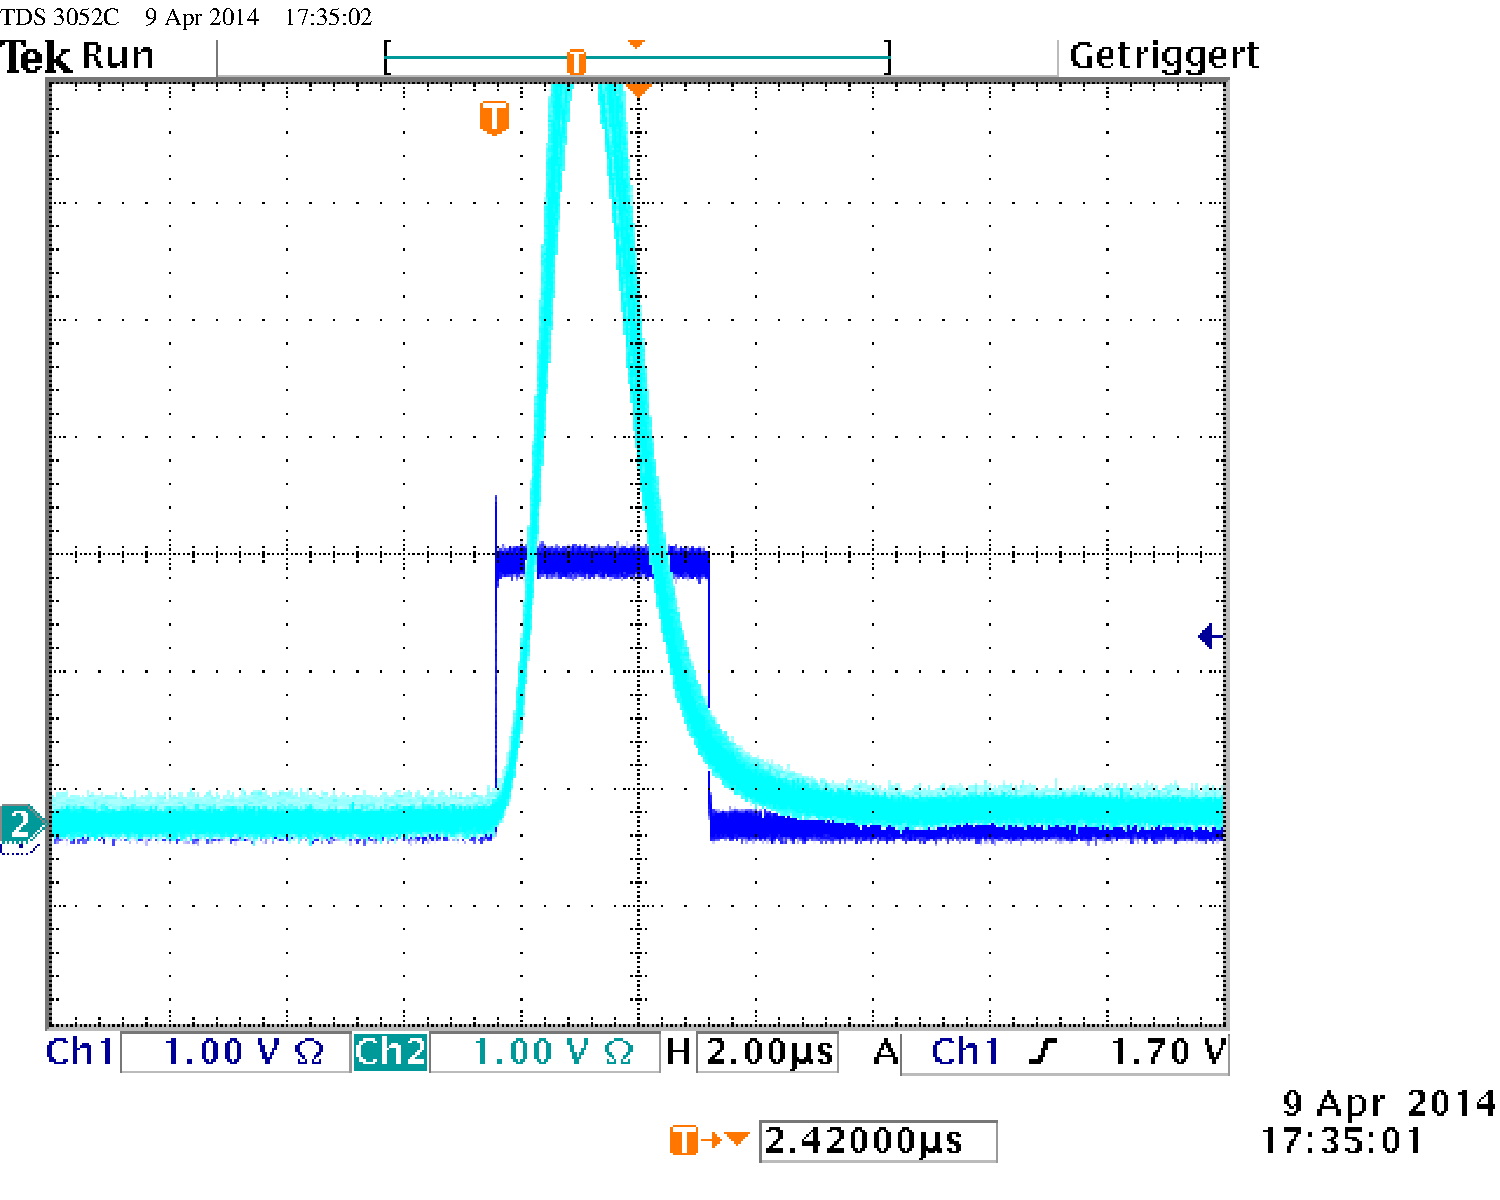
\includegraphics[width=0.49\linewidth]{../Daten/2014-04-09_17-35-east.pdf}
    \hfill
    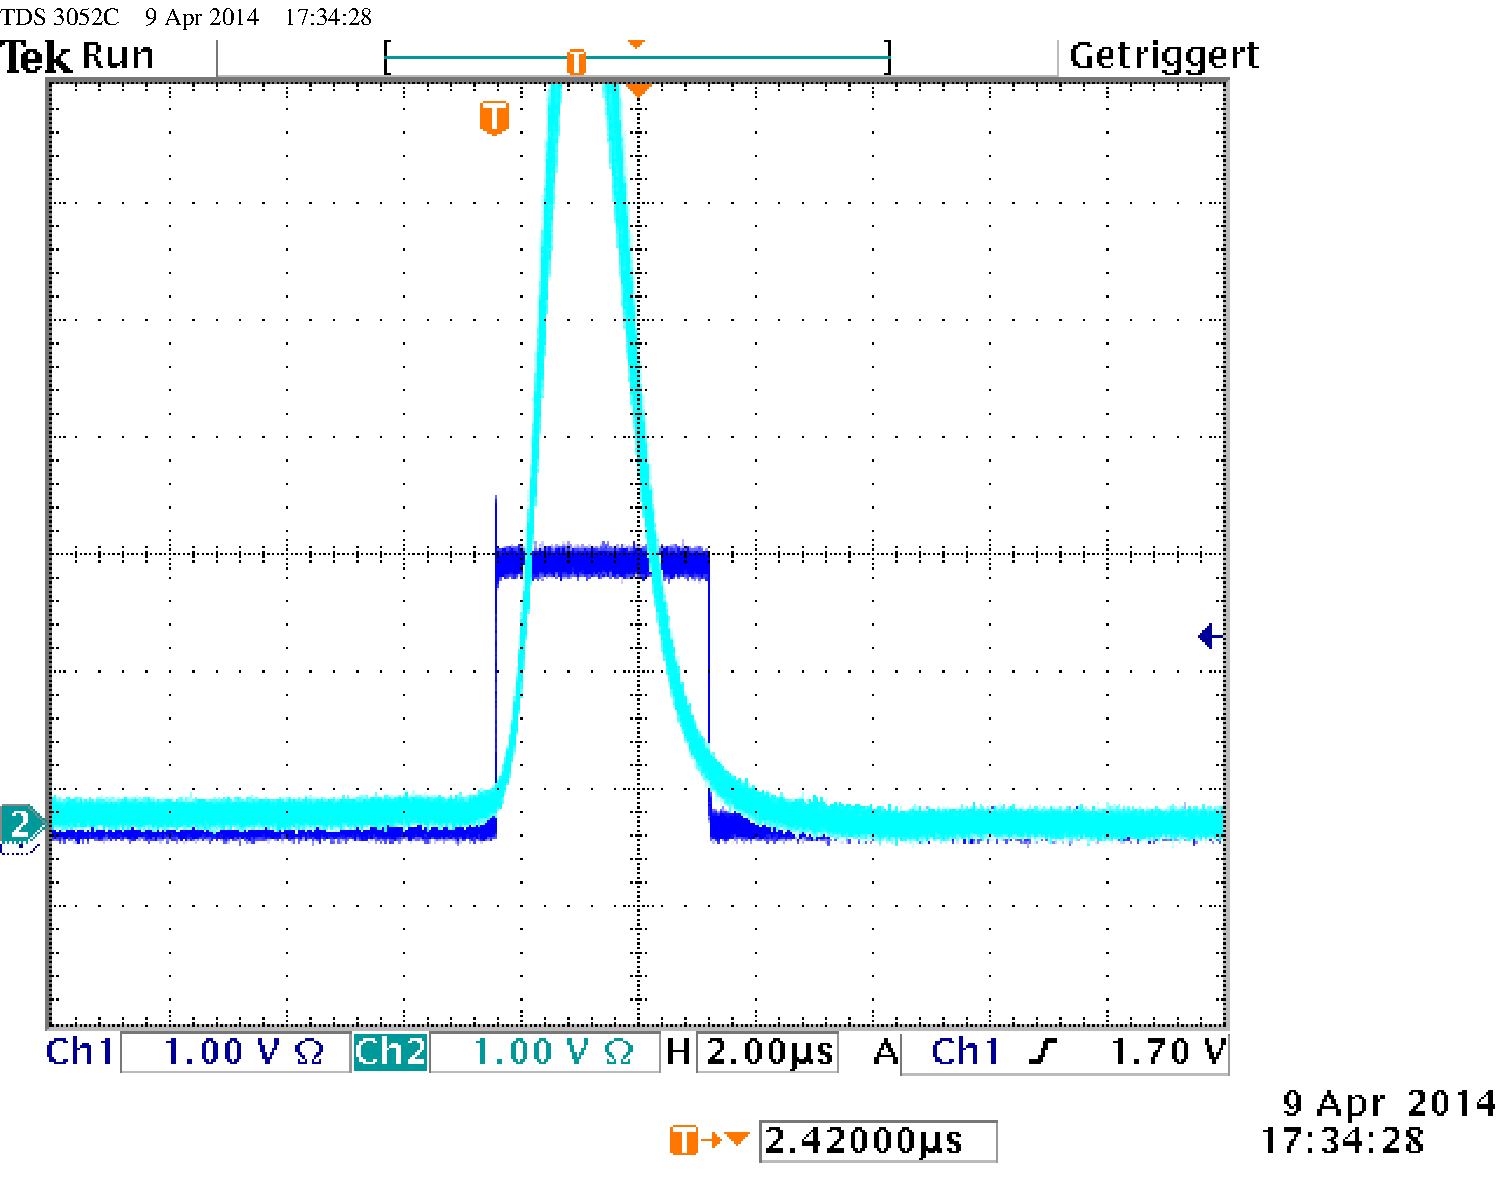
\includegraphics[width=0.49\linewidth]{../Daten/2014-04-09_17-34-east.pdf}
    \caption{%
        Durch den auf die \SI{511}{\kilo\electronvolt}-Linie eingestellten SCA
        erhalten wir im Oszilloskop mit dem Trigger auf dem zweiten Kanal nur
        noch eine Pulshöhe.
    }
    \label{fig:eine_pulshoehe}
\end{figure}

\subsection{Slow-Koinzidenz herstellen}

Wir schließen beide SCAs gleichzeitig an das Oszilloskop an. Der rechte Detektor
ist auf Kanal 1/* Bildzeit 17:38 */, siehe Abbildung~\ref{fig:beide_sca}. Die
beiden Signale liegen ausreichend genau aufeinander, es herrscht Koinzidenz.

\begin{figure}[htbp]
    \centering
    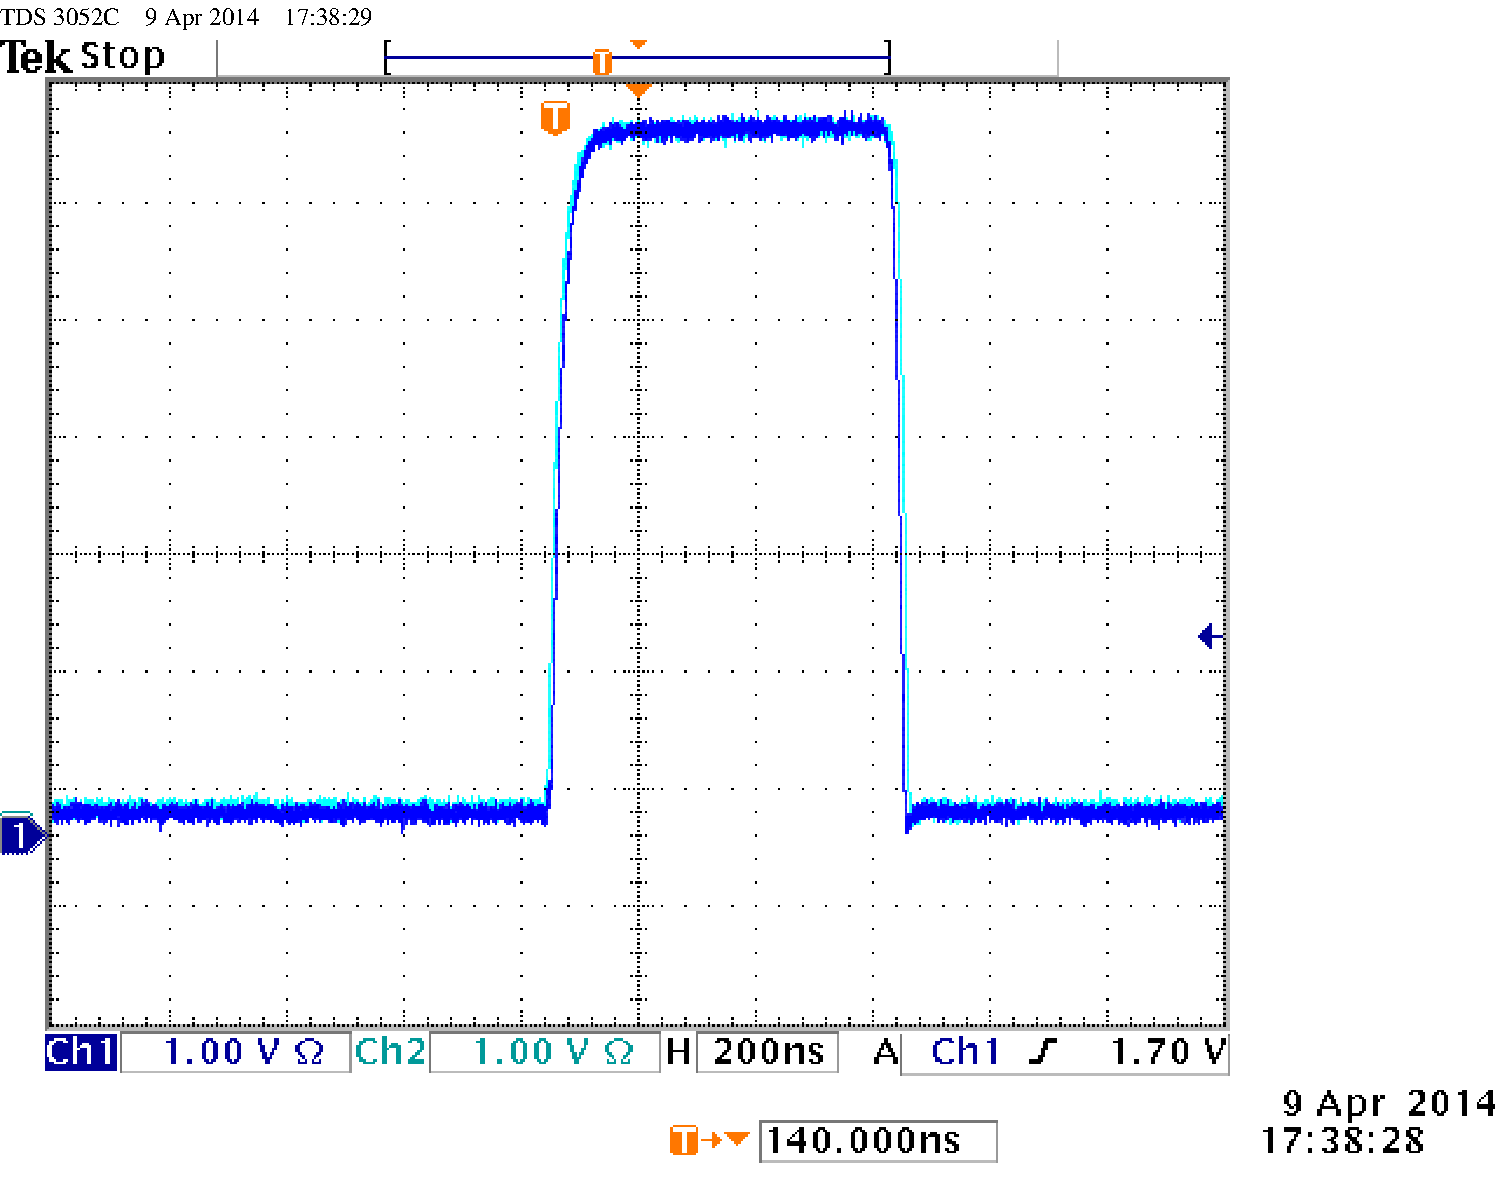
\includegraphics[width=0.49\linewidth]{../Daten/2014-04-09_17-38-east.pdf}
    \hfill
    \caption{%
        Die Signale von beiden SCA gleichzeitig auf dem Oszilloskop.
    }
    \label{fig:beide_sca}
\end{figure}

\section{Fast-Konzidenzkreis einstellen}

Wir beginnen mit der Einstellung des Fast-Kreises am rechten Detektor. Wir
betrachten das Slow-Signal nach dem Vorverstärker und das Fast-Signal zusammen
auf dem Oszilloskop/*Bildzeit 09:27*/, siehe
Abbildung~\ref{fig:fast_einstellen}. Das gleiche wiederholen wir für den linken
Detektor/*Bildzeit 09:29*/.

\begin{figure}[htbp]
    \centering
    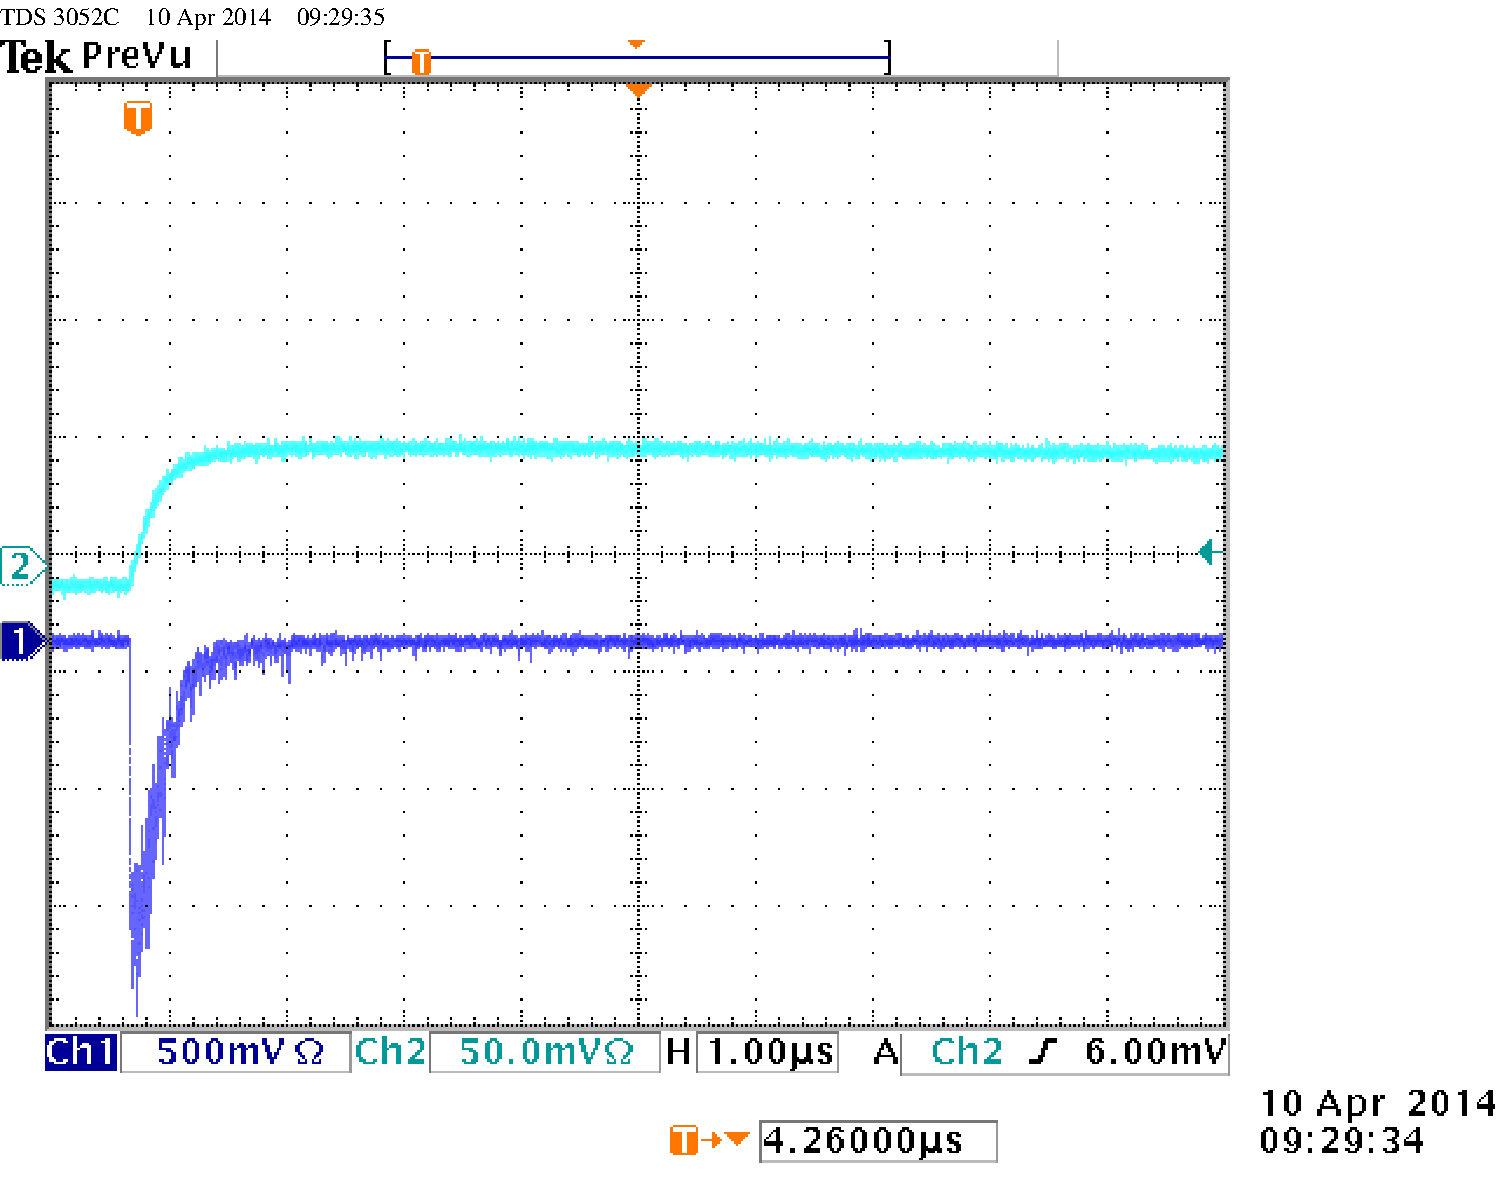
\includegraphics[width=0.49\linewidth]{../Daten/2014-04-10_09-29-34-east.pdf}
    \hfill
    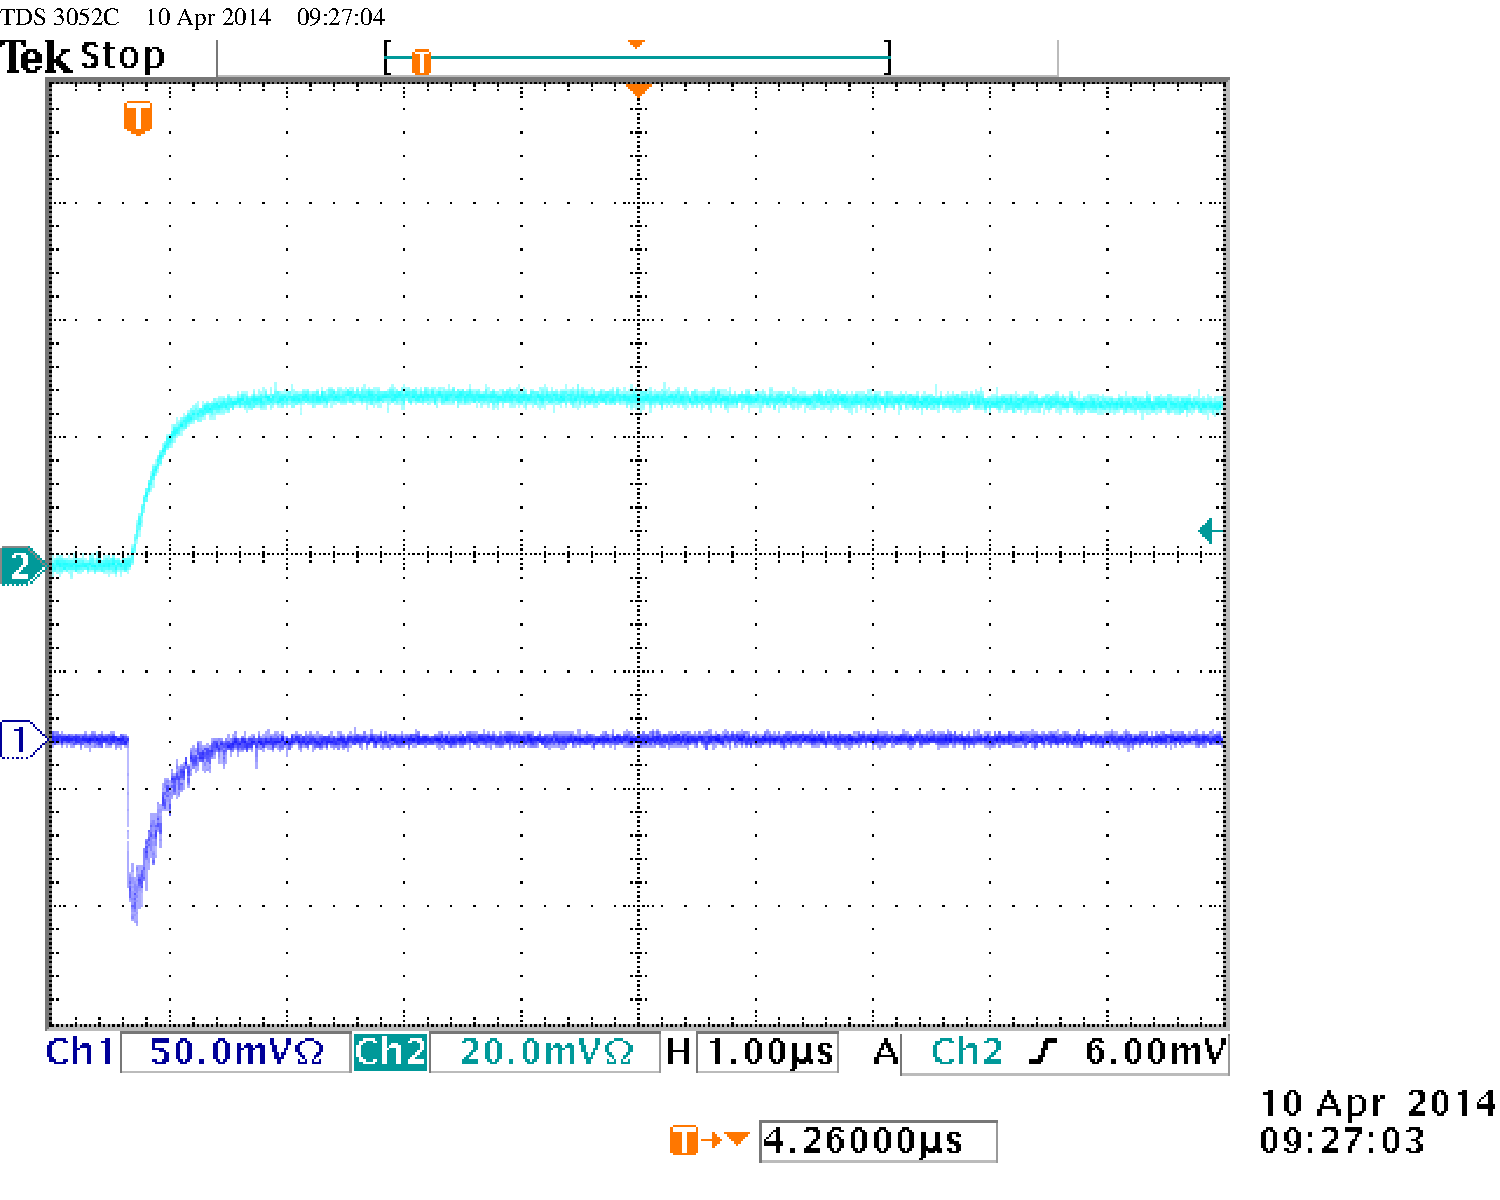
\includegraphics[width=0.49\linewidth]{../Daten/2014-04-10_09-27-east.pdf}
    \caption{%
        Slow-Signal nach dem Vorverstärker zusammen mit dem Fast-Signal des
        gleichen Detektors, jeweils für den linken und rechten Zweig.
    }
    \label{fig:fast_einstellen}
\end{figure}

Dann schließen wir den linken Hauptverstärker über das Delay an das Oszilloskop
an. Das Signal des rechten Fast-Ausgangs wird an das CFD und dessen negativer
Ausgang an das Oszilloskop angeschlossen, siehe
Abbildung~\ref{fig:aufbau:fast1}.

\begin{figure}[htbp]
    \centering
    \begin{tikzpicture}
        \node[device] (na) {$^{22}\mathrm{Na}$};
        \node[device] (pm) [right=of na] {Photomultiplier};
        \node[device] (amp) [right=of pm] {Verstärker};
        \node[device] (delay) [right=of amp] {Delay};
        \node[device] (cfd) [below=of pm] {CFD};
        \node[monitor] (oszi) [below=of delay] {Oszilloskop};

        % Teilchenaustausch
        \begin{scope}[->, dotted, thick]
            \draw (na) -- (pm);
        \end{scope}

        % Analogsignal
        \begin{scope}[->]
            \draw (pm) -- (amp);
            \draw (amp) -- (delay);
            \draw (delay) -- (oszi);
            \draw (pm) -- (cfd);
        \end{scope}

        % Digitalsignal
        \begin{scope}[->, dashdotted]
            \draw (cfd) -- (oszi);
        \end{scope}
    \end{tikzpicture}
    \caption{%
        Erster Aufbau zur Einstellung des Fast-Kreises.
    }
    \label{fig:aufbau:fast1}
\end{figure}

Wir nehmen ein Bild mit Baseline auf/*Bild 09:50*/, siehe
Abbildung~\ref{fig:cfd_einstellen_baseline}. Nun erhöhen wir die Schwelle am
CFD auf \num{0.4}, so dass die Baseline verschwindet/*Bild 09:51*/, siehe
Abbildung~\ref{fig:cfd_einstellen}. Dies wiederholen wir für den rechten Zweig.
Beim rechten CFD hat schon bei unterster Schwelleneinstellung keine
Baseline/*Bild 10:17*/, siehe Abbildung~\ref{fig:cfd_einstellen}. Daher werden
wir den linken CFD als Stop-Signal zu benutzen, damit wir die
\SI{81}{\kilo\electronvolt}-Linie nicht abschneiden.

\begin{figure}[htbp]
    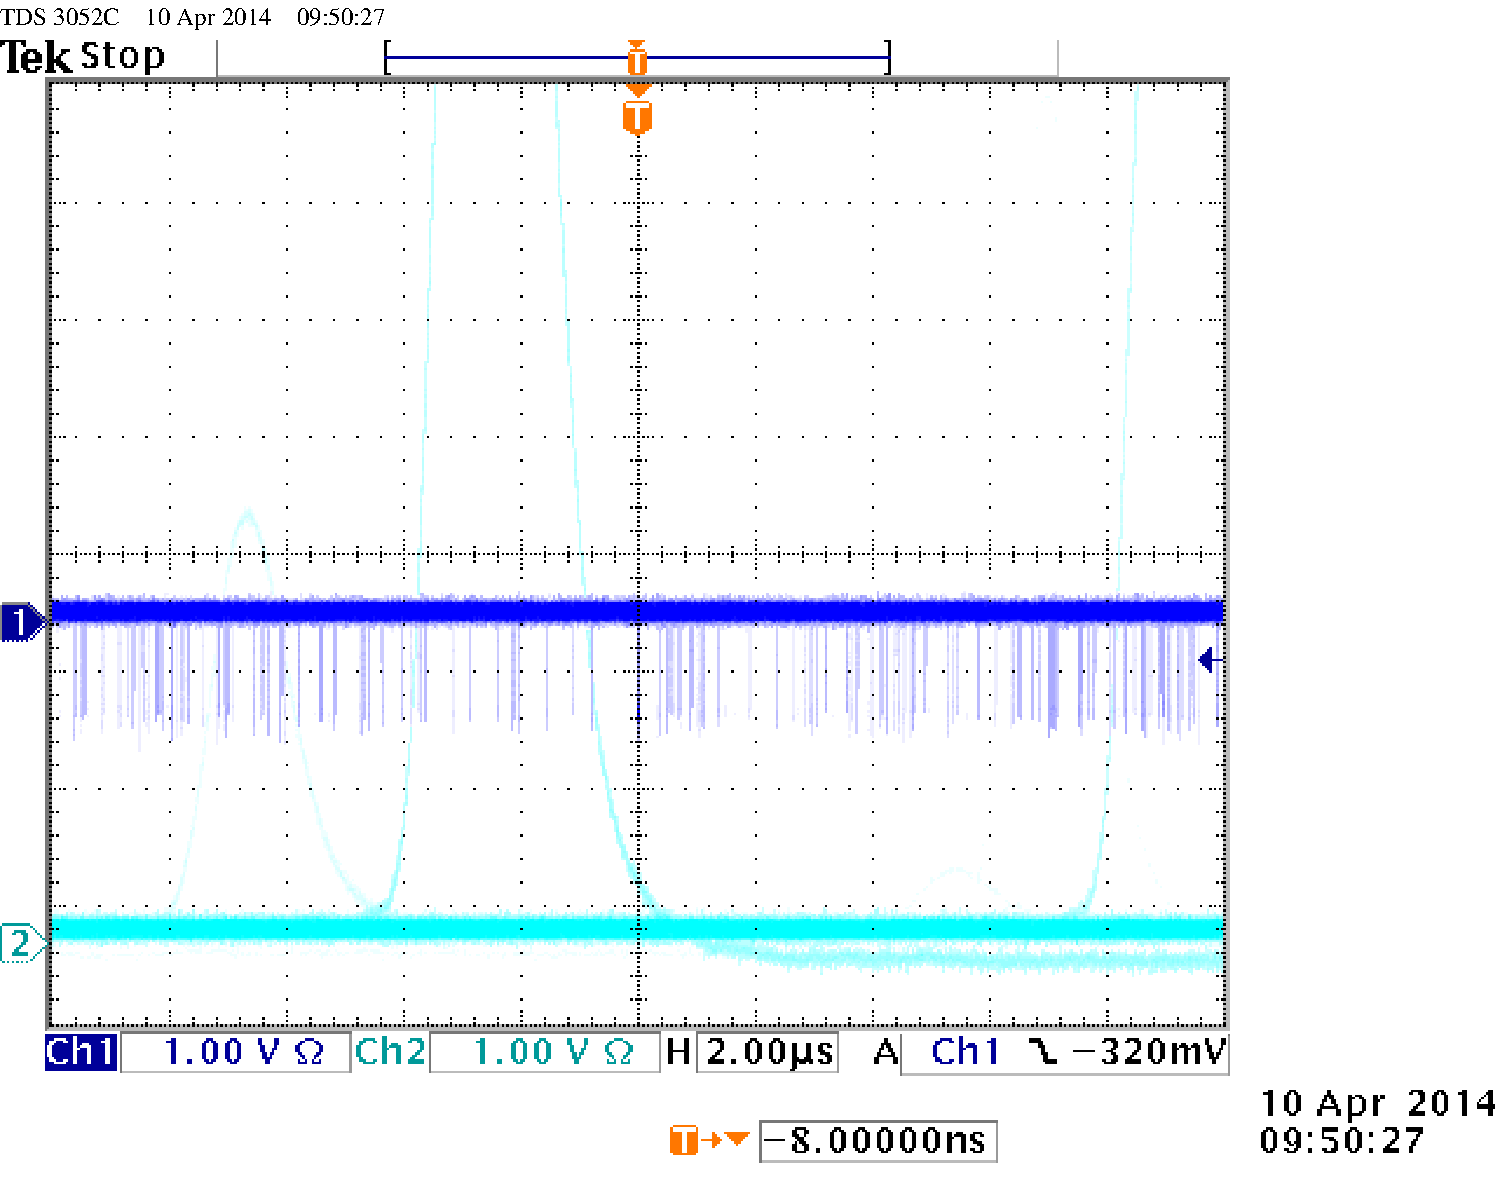
\includegraphics[width=0.49\linewidth]{../Daten/2014-04-10_09-50-east.pdf}
    \caption{%
        Fast- und Slow-Signal mit Baseline.
    }
    \label{fig:cfd_einstellen_baseline}
\end{figure}

\begin{figure}[htbp]
    \centering
    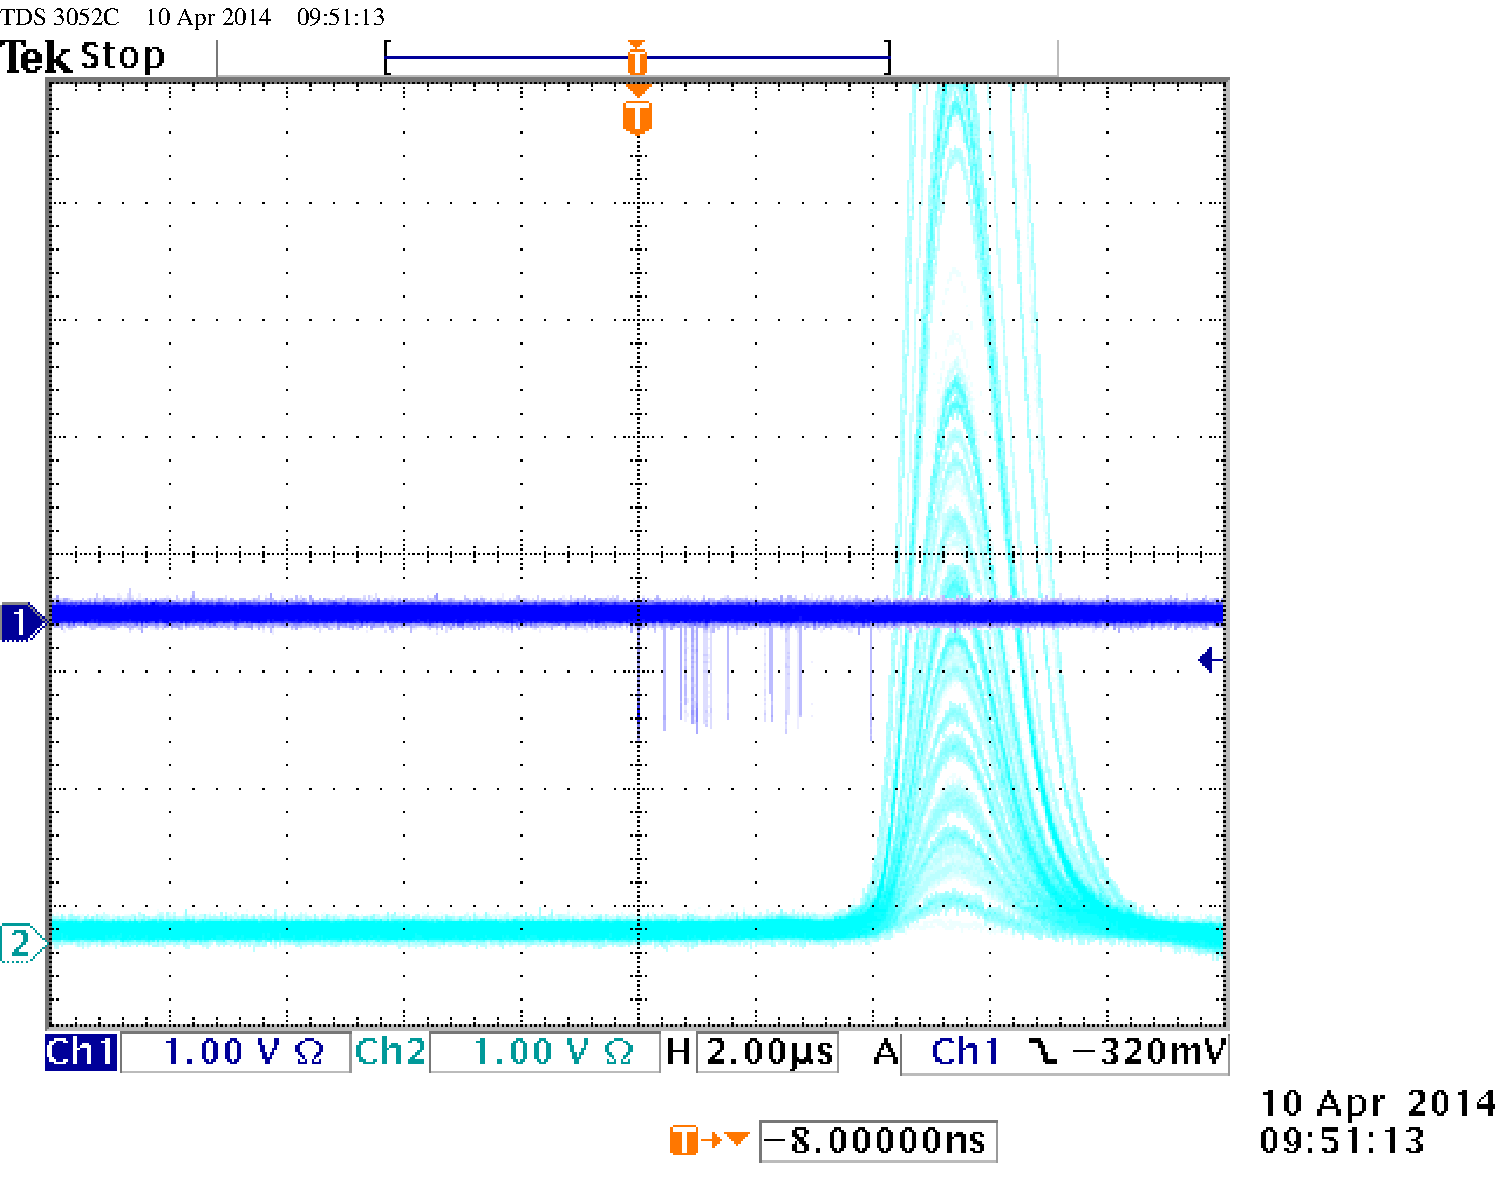
\includegraphics[width=0.49\linewidth]{../Daten/2014-04-10_09-51-east.pdf}
    \hfill
    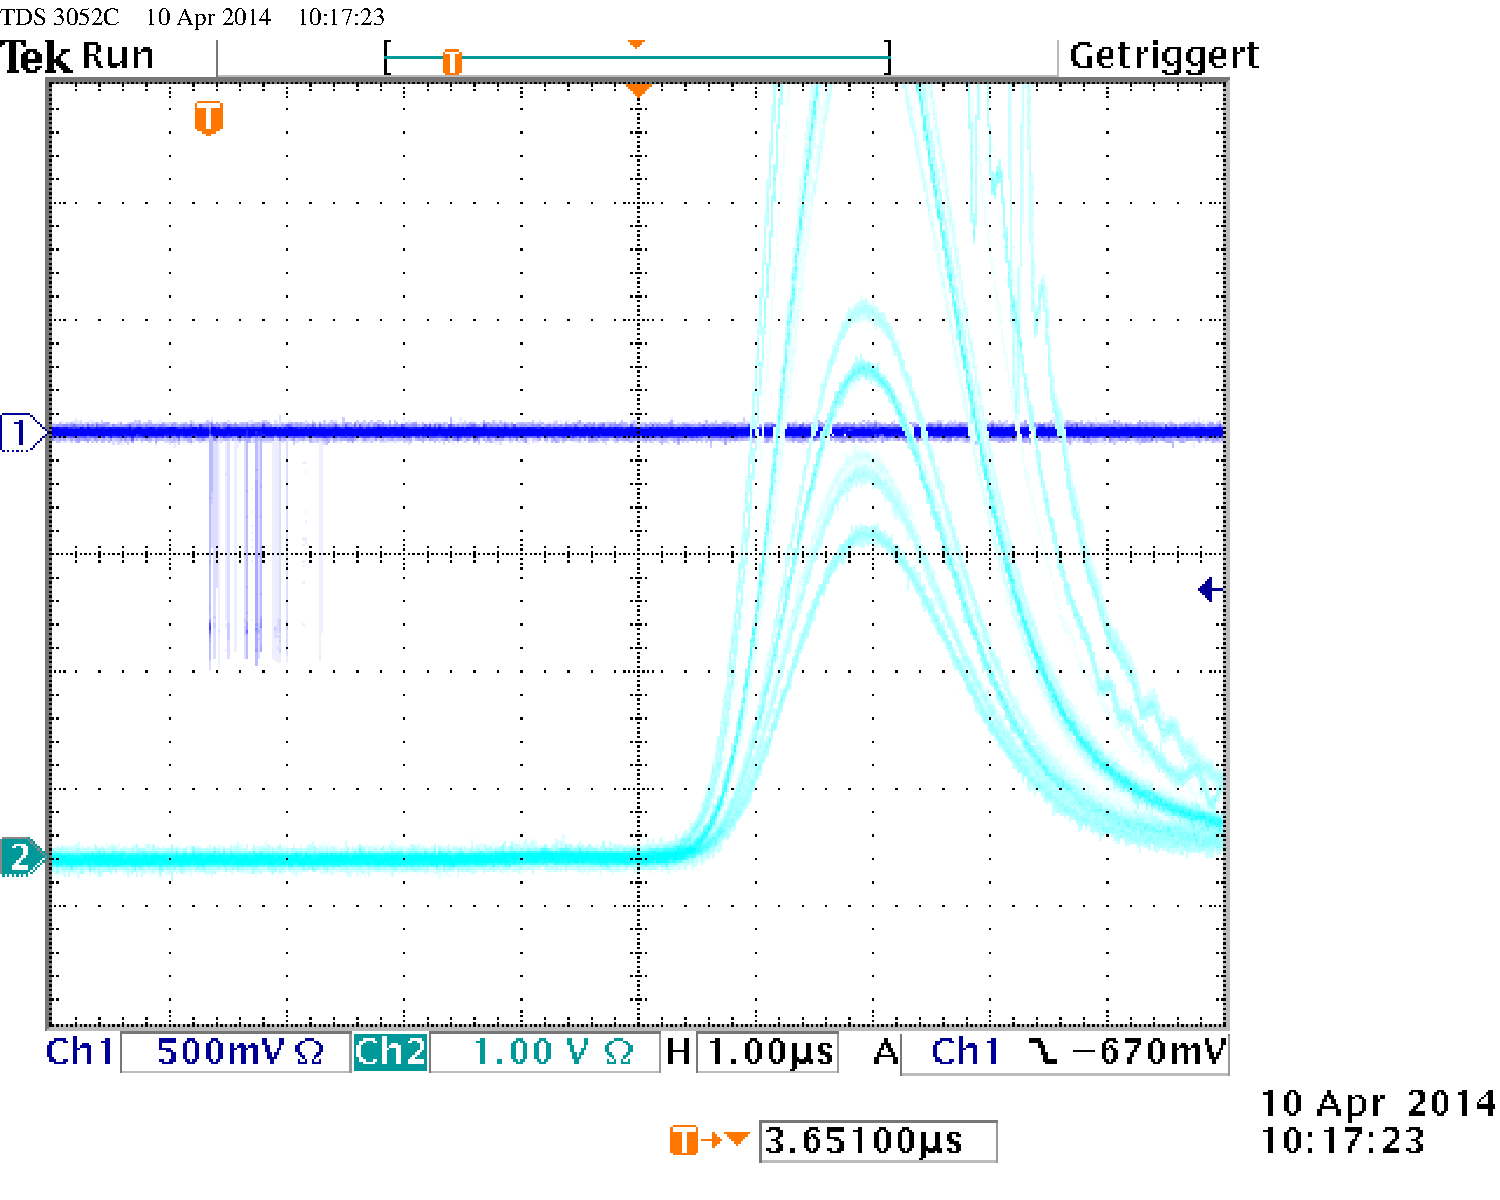
\includegraphics[width=0.49\linewidth]{../Daten/2014-04-10_10-17-23-east.pdf}
    \caption{%
        Fast- und Slow-Signal mit herausgefilterter Baseline für linken und
        rechten Detektor.
    }
    \label{fig:cfd_einstellen}
\end{figure}

Es ist gut zu erkennen, dass Triggerung erst dann gut funktioniert, wenn das
Rauschen in der Baseline ignoriert wird und nur starke Signale einen Logikpuls
auslösen.

Wir schließen den CFD, den wir für das Stop-Signal nutzen wollen, noch an ein
Delay an. Delay und den Start-CFD geben wir auf das Oszilloskop/*Bildzeit
10:27*/, siehe Abbildung~\ref{fig:aufbau:fast2}. Das Oszillogramm ist in
Abbildung~\ref{fig:cfd_stop} gezeigt. Danach geben wir beide CFD Signale
(mit Delay) auf das TAC, siehe Abbildung~\ref{fig:aufbau:fast3}.

\begin{figure}[htbp]
    \centering
    \begin{tikzpicture}
        \node[device] (na) {$^{22}\mathrm{Na}$};
        \node[device] (pm1) [above=of na] {Photomultiplier};
        \node[device] (pm2) [below=of na] {Photomultiplier};
        \node[device] (cfd1) [right=of pm1] {CFD};
        \node[device] (cfd2) [right=of pm2] {CFD};
        \node[device] (delay) [right=of cfd2] {Delay};
        \node[monitor] (oszi) [above=of delay] {Oszilloskop};

        % Teilchenaustausch
        \begin{scope}[->, dotted, thick]
            \draw (na) -- (pm1);
            \draw (na) -- (pm2);
        \end{scope}

        % Analogsignal
        \begin{scope}[->]
            \draw (pm1) -- (cfd1);
            \draw (pm2) -- (cfd2);
        \end{scope}

        % Digitalsignal
        \begin{scope}[->, dashdotted]
            \draw (cfd1) -- (oszi);
            \draw (cfd2) -- (delay);
            \draw (delay) -- (oszi);
        \end{scope}
    \end{tikzpicture}
    \caption{%
        Aufbau zum Bestimmen des benötigten Delays hinter dem Stop-CFD.
    }
    \label{fig:aufbau:fast2}
\end{figure}

\begin{figure}[htbp]
    \centering
    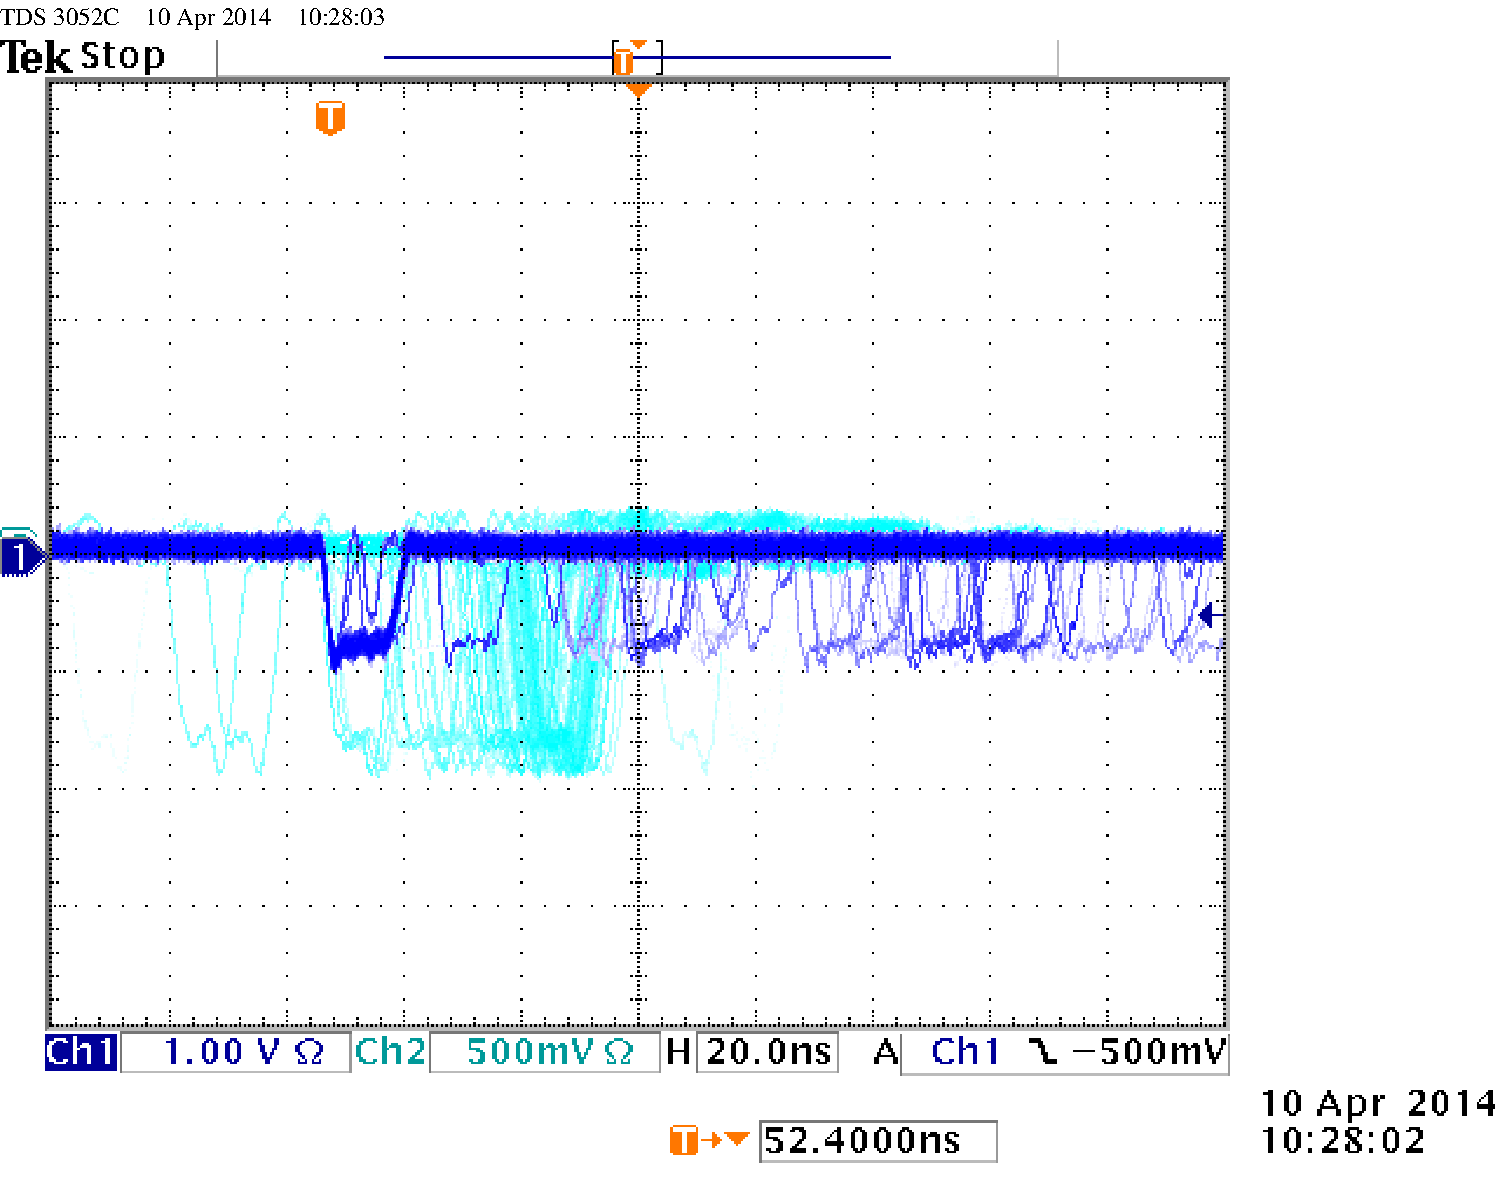
\includegraphics[width=0.49\linewidth]{../Daten/2014-04-10_10-28-east.pdf}
    \caption{%
        Signale Start- und Stop-CFDs zusammen.
    }
    \label{fig:cfd_stop}
\end{figure}

Durch die zusätzliche Verzögerung hinter dem Stop-CFD erscheinen dessen Pulse
sichtbar weiter hinter den Pulse des Start-CFD. Auf diese Weise ist
sichergestellt, dass das TAC richtig arbeiten kann.

\begin{figure}[htbp]
    \centering
    \begin{tikzpicture}
        \node[device] (na) {$^{22}\mathrm{Na}$};
        \node[device] (pm1) [above=of na] {Photomultiplier};
        \node[device] (pm2) [below=of na] {Photomultiplier};
        \node[device] (cfd1) [right=of pm1] {CFD};
        \node[device] (cfd2) [right=of pm2] {CFD};
        \node[device] (delay) [right=of cfd2] {Delay};
        \node[device] (tac) [above=of delay] {TAC};
        \node[monitor] (oszi) [right=of tac] {Oszilloskop};

        % Teilchenaustausch
        \begin{scope}[->, dotted, thick]
            \draw (na) -- (pm1);
            \draw (na) -- (pm2);
        \end{scope}

        % Analogsignal
        \begin{scope}[->]
            \draw (pm1) -- (cfd1);
            \draw (pm2) -- (cfd2);
            \draw (tac) -- (oszi);
        \end{scope}

        % Digitalsignal
        \begin{scope}[->, dashdotted]
            \draw (cfd1) -- (tac);
            \draw (cfd2) -- (delay);
            \draw (delay) -- (tac);
        \end{scope}
    \end{tikzpicture}
    \caption{%
    }
    \label{fig:aufbau:fast3}
\end{figure}

\section{Zeiteichung des TAC}

Wir prüfen erneut die Slow-Koinzidenz/* Bildzeit 10:39, um 13:10 jedoch noch
mal richtig gemacht */, siehe Abbildung~\ref{fig:pruef_slow}.

\begin{figure}[htbp]
    \centering
    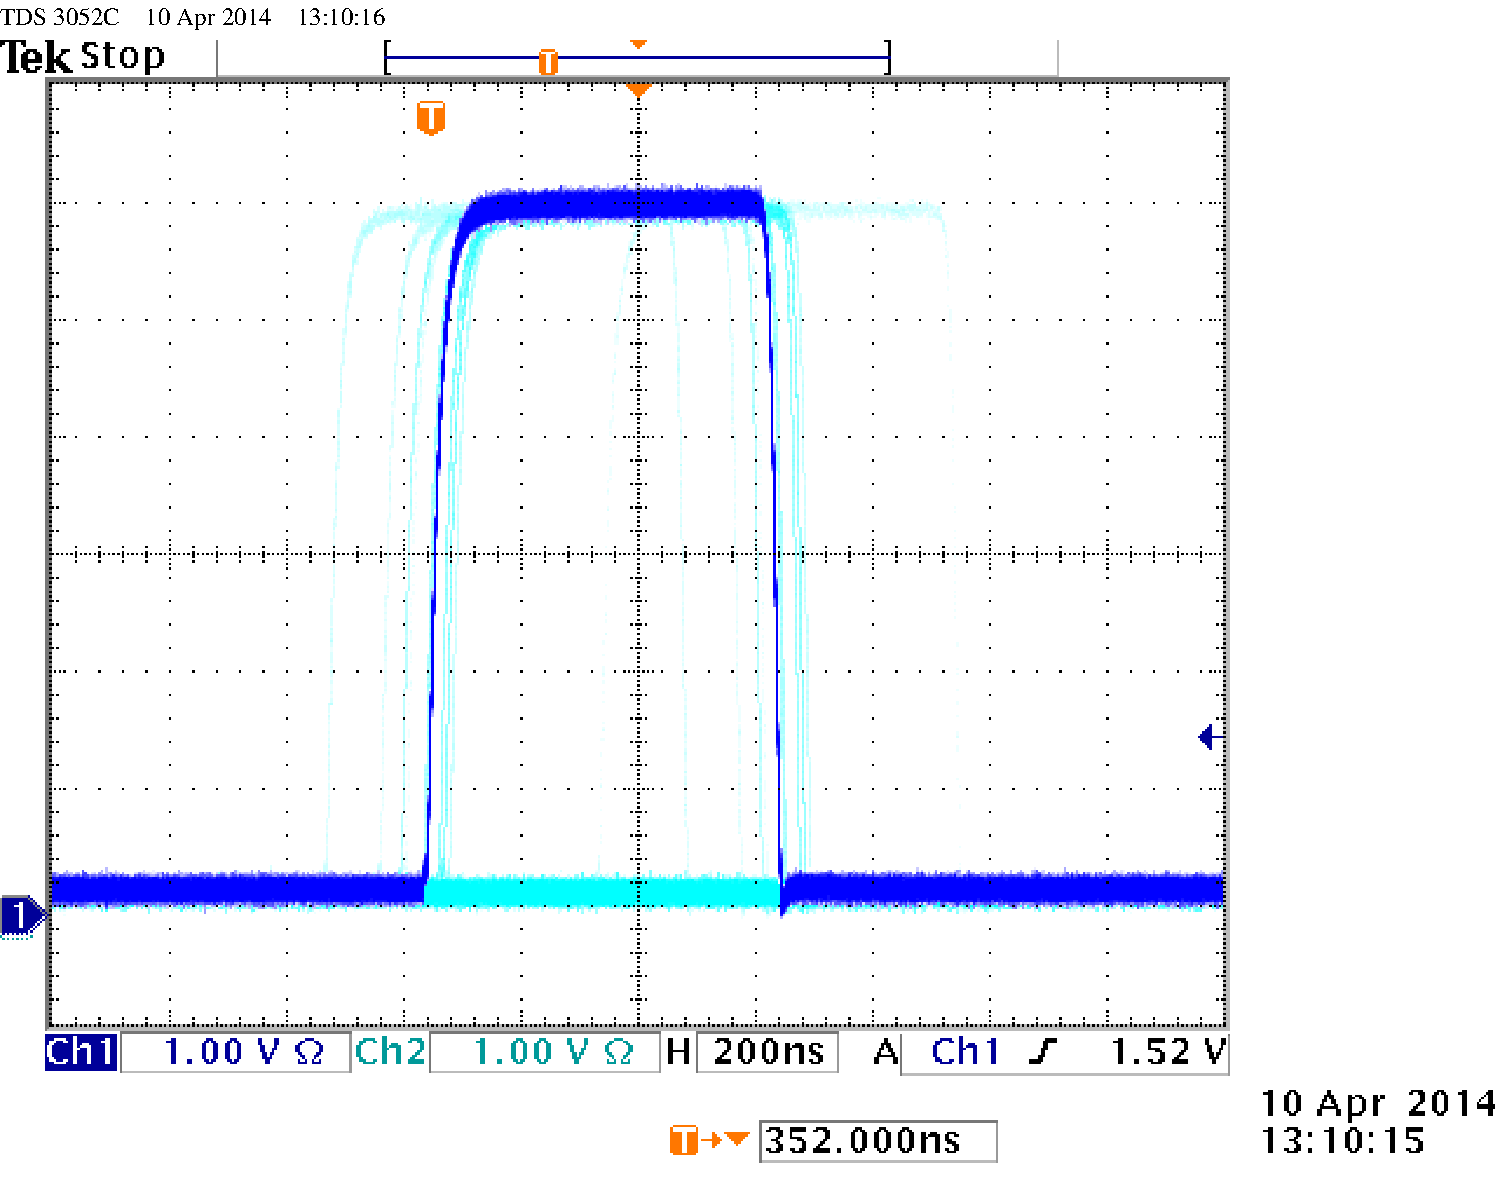
\includegraphics[width=0.49\linewidth]{../Daten/2014-04-10_13-10-east.pdf}
    \caption{%
        Überprüfung der Slow-Koinzidenz.
    }
    \label{fig:pruef_slow}
\end{figure}

Die Signale der SCAs überlappen sich noch immer ausreichend, so dass die
Koinzidenz weiterhin besteht.

Dann schließen wir die zwei SCAs an die Koinzidenzeinheit an. Diese dann an das
GDG und dieses an das Oszilloskop. Das TAC kommt an den zweiten Kanal/*
Bildzeit 10:49 */, siehe Abbildung~\ref{fig:tac_oszi}.

\begin{figure}[htbp]
    \centering
    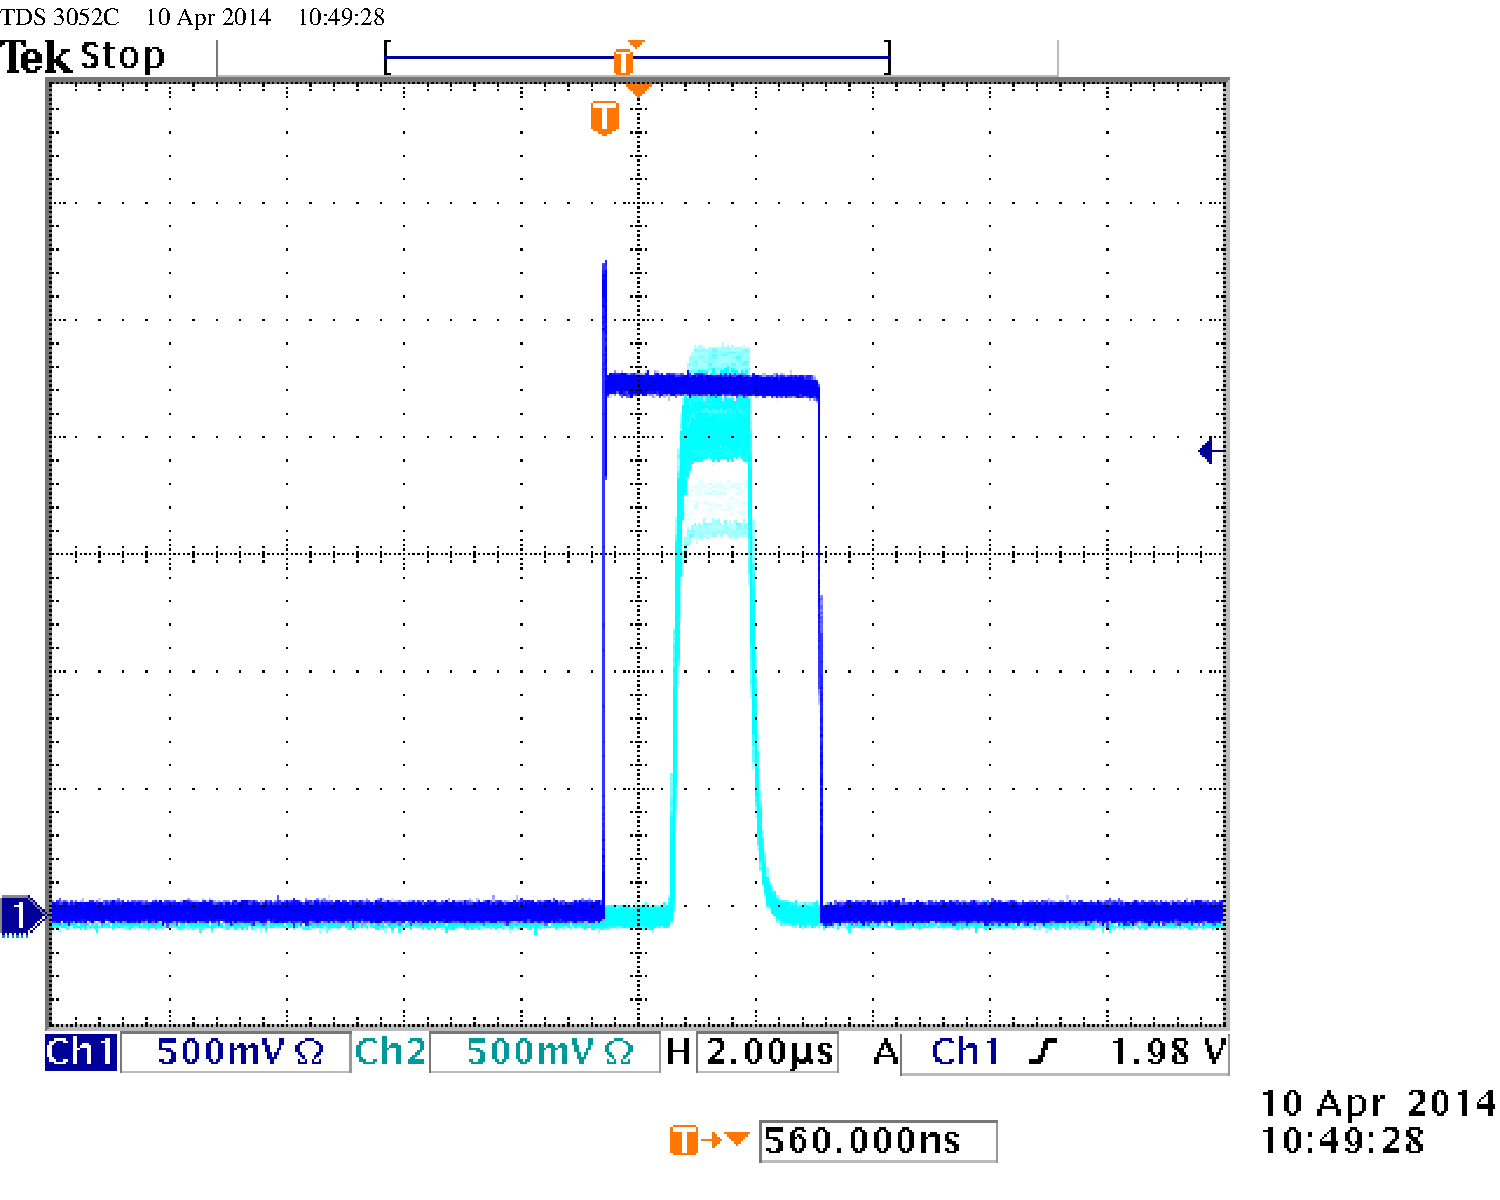
\includegraphics[width=0.49\linewidth]{../Daten/2014-04-10_10-49-28-east.pdf}
    \caption{%
    }
    \label{fig:tac_oszi}
\end{figure}

Hier ist gut zu erkennen, dass die Slow- und die Fast-Koinzidenz überlappen.
So wird die Datennahme mit dem MCA später funktionieren. Im zweiten Kanal sind
verschiedene Amplituden zu erkennen. Es gibt also verschiedene Lebensdauern,
und man kann sie hier sehen.

Zuletzt schließen wir den GDG und das TAC an das MCA an (Aufbau in
Abbildung~\ref{fig:aufbau:komplett}) und nehmen Promptkurven auf, siehe
Abbildung~\ref{mca:zeiteichung}.

\begin{figure}[htbp]
    \centering
    \begin{tikzpicture}
        \node[device] (koinzidenz) at (10, 0) {Koinzidenzeinheit};
        \node[device] (gdg) [right=of koinzidenz] {GDG};
        \node[device] (mca) [above=of gdg] {MCA};

        \begin{scope}[start chain, node distance=5mm, every node/.style={join}, every join/.style={->}]
            \node[device, on chain] (22Na) at (0, 0) {$^{22}\mathrm{Na}$};

            \begin{scope}[start branch=22Na]
                \node[device, on chain=going below, node distance=1.5cm] (Szintillator1) {Szintillator};
                \node[device, on chain] (PM2) {Photomultiplier};

                \begin{scope}[start branch=PM2]
                    \node[device, on chain=going below right] (amp2) {Verstärker};
                    \node[device, on chain] (splitter2) {Splitter};
                    \begin{scope}[start branch=splitter2]
                        \node[device, on chain=going below right] (delay2) {Verzögerung};
                    \end{scope}
                    \begin{scope}[start branch=splitter2]
                        \node[device, on chain=going above right] (sca2) {SCA};
                    \end{scope}

                \end{scope}
                \node[device, on chain=going above right] (cfd2) {CFD};
                \node[device, on chain] (cfddelay) {Verzögerung};
            \end{scope}

            \node[device, on chain=going above, node distance=1.5cm] (Szintillator1) {Szintillator};
            \node[device, on chain] (PM1) {Photomultiplier};

            \begin{scope}[start branch=PM1]
                \node[device, on chain=going above right] (amp1) {Verstärker};
                \node[device, on chain] (splitter1) {Splitter};
                \begin{scope}[start branch=splitter1]
                    \node[device, on chain=going above right] (delay1) {Verzögerung};
                \end{scope}
                \begin{scope}[start branch=splitter1]
                    \node[device, on chain=going below right] (sca1) {SCA};
                \end{scope}
            \end{scope}

            \node[device, on chain=going below right] (cfd1) {CFD};
            \node[device, on chain=going right, node distance=2cm, join=with cfddelay] (tac) {TAC};

        \end{scope}

        \begin{scope}[->]
            \draw (tac) -- (mca);

            \begin{scope}[dashdotted]
                \draw (gdg) -- (mca);
                \draw (sca1) -- (koinzidenz);
                \draw (koinzidenz) -- (gdg);
                \draw (sca2) -- (koinzidenz);
            \end{scope}
        \end{scope}
    \end{tikzpicture}
    \caption{%
        Kompletter Aufbau
    }
    \label{fig:aufbau:komplett}
\end{figure}

\begin{figure}[htbp]
    \centering
    \begin{tikzpicture}
        \begin{axis}[
                width=\linewidth, height=0.3\linewidth, xlabel=Kanal,
                ylabel=Ereignisse, axis lines=left, xtick={0,1000,...,8000}
            ]
            \addplot[black] table {../Daten/Zeiteichung.txt};
        \end{axis}
    \end{tikzpicture}
    \caption{%
        Promptkurve des TAC.
    }
    \label{mca:zeiteichung}
\end{figure}

Mit diesen Promptkurven werden wir nachher die Beziehung zwischen MCA-Kanälen
und Zeitdifferenzen herstellen können.

\section{Messung der Lebensdauer}

Wir tauschen die Natrium- gegen die Bariumquelle aus. Das rechte Slow-Signal
geben wir mit Splitter einmal auf den SCA und dann auf den GDG, das andere über
das Delay und beide auf das Oszilloskop. Die Signale werden übereinander
gelegt/* Bildzeit rechts 12:28, links 12:27 */, siehe
Abbildung~\ref{fig:eine_pulshoehe_ba}. Dies wiederholen wir mit dem linken
Zweig.

\begin{figure}[htbp]
    \centering
    %\includegraphics[width=0.49\linewidth]{../Daten/2014-04-10_12-27-east.pdf}
    \hfill
    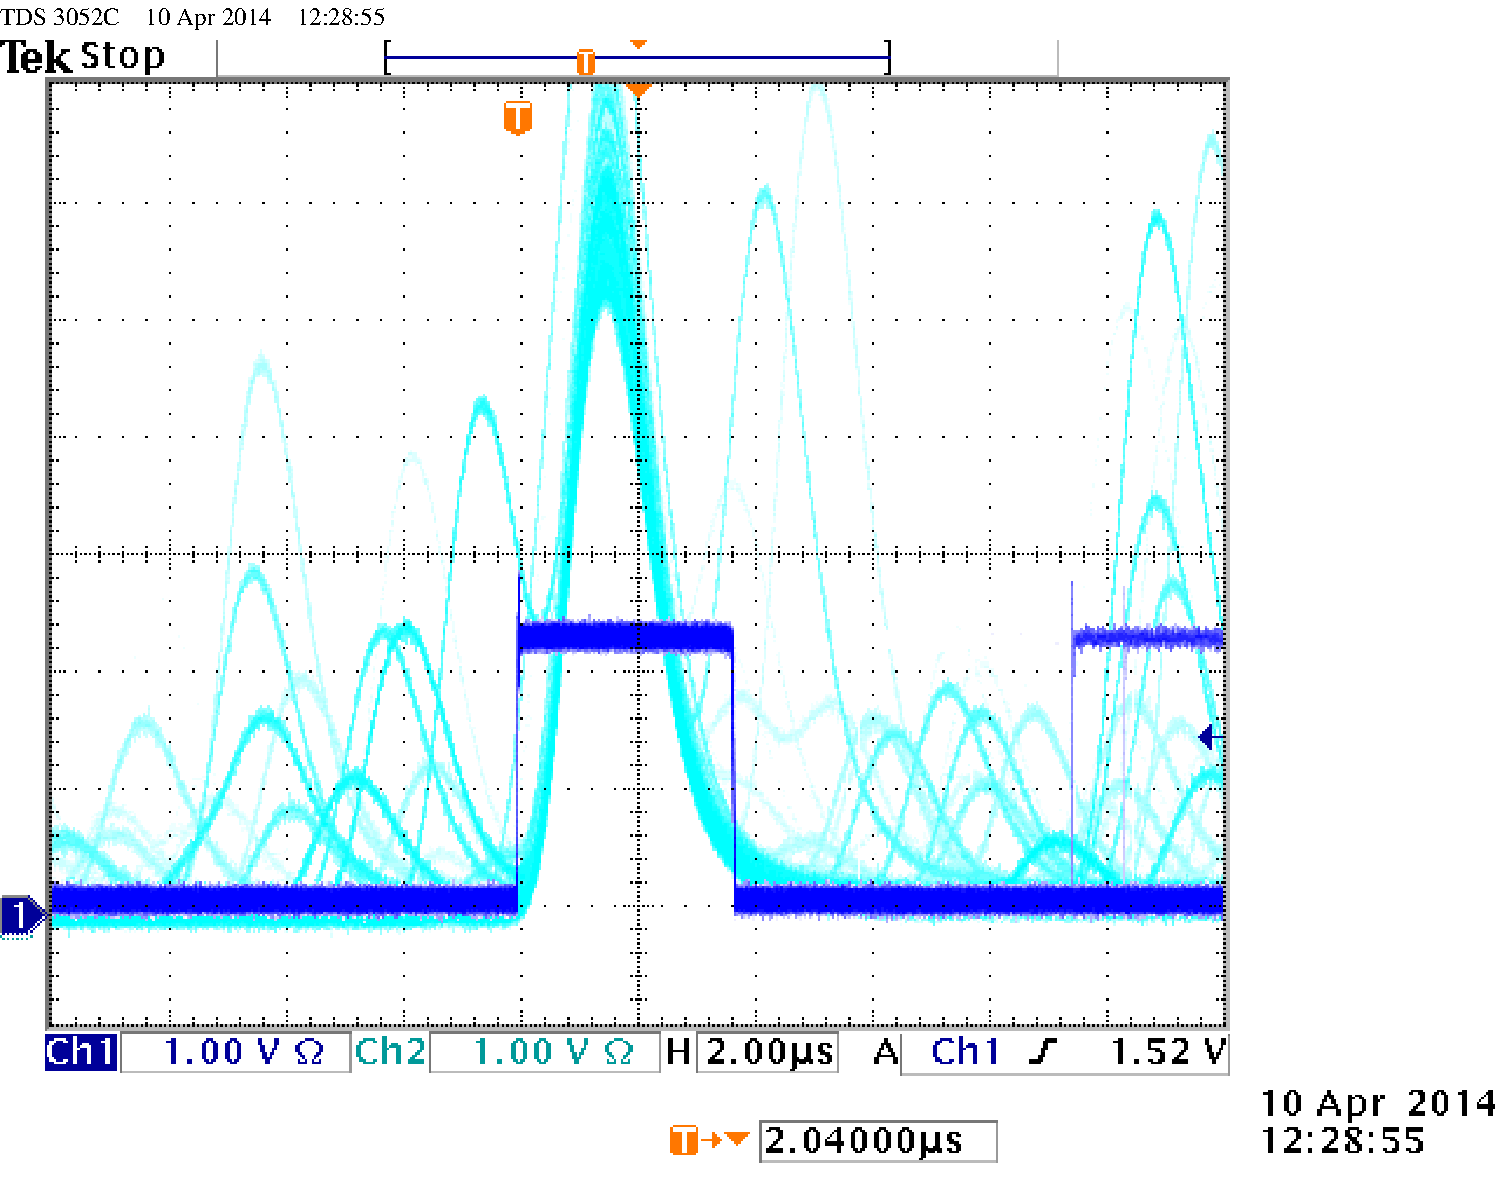
\includegraphics[width=0.49\linewidth]{../Daten/2014-04-10_12-28-east.pdf}
    \caption{%
        SCA- gegen Slow-Signal für den rechten Detektor mit der Bariumquelle.
    }
    \label{fig:eine_pulshoehe_ba}
\end{figure}

Dann wird ein Spektrum mit dem MCA aufgenommen/* 009 */, siehe Abbildung~\ref{mca:ba_spek}.

\begin{figure}[htbp]
    \centering
    \begin{tikzpicture}
        \begin{axis}[width=0.45\linewidth, height=0.3\linewidth, xlabel=Kanal, ylabel=Ereignisse, axis lines=left]
            \addplot[black] table {../Daten/011-Ba-Spek-l.txt};
        \end{axis}
    \end{tikzpicture}
    \hfill
    \begin{tikzpicture}
        \begin{axis}[width=0.45\linewidth, height=0.3\linewidth, xlabel=Kanal, ylabel=Ereignisse, axis lines=left]
            \addplot[black] table {../Daten/009-Ba-Spek-r.txt};
        \end{axis}
    \end{tikzpicture}
    \caption{%
        Spektrum der Bariumemissionen im linken und rechten Detektor.
    }
    \label{mca:ba_spek}
\end{figure}

Dann wird SCA Fenster so eingestellt, dass die nur
\SI{350}{\kilo\electronvolt}-Linie drin ist/* 010 */, siehe
Abbildung~\ref{mca:ba_spek_sca}.

\begin{figure}[htbp]
    \centering
    \begin{tikzpicture}
        \begin{axis}[width=0.45\linewidth, height=0.3\linewidth, xlabel=Kanal, ylabel=Ereignisse, axis lines=left]
            \addplot[black] table {../Daten/012-Ba-SCA-l.txt};
        \end{axis}
    \end{tikzpicture}
    \hfill
    \begin{tikzpicture}
        \begin{axis}[width=0.45\linewidth, height=0.3\linewidth, xlabel=Kanal, ylabel=Ereignisse, axis lines=left]
            \addplot[black] table {../Daten/014-Ba-SCA-r2.txt};
        \end{axis}
    \end{tikzpicture}
    \caption{%
        Einstellung der SCA Schwellen, so dass nur die gewünschte Linie wächst.
    }
    \label{mca:ba_spek_sca}
\end{figure}

Mit dem linken Slow-Zweig gehen wir gleich vor, wir nehmen ein Spektrum/* 011
*/ und kalibrieren das SCA Fenster/* 012 */ auf die andere Linie. Siehe
ebenfalls Abbildungen \ref{mca:ba_spek} und \ref{mca:ba_spek_sca}.

Wir betrachten das rechte Slow-Signal und Start-CFD-Signal auf dem
Oszilloskop/*Bildzeit 13:18*/. Die Schwelle des CFD stellen wir auf das
Minimum. Dann wechseln wir auf den Stop-Zweig (links) und betrachten zuerst
ohne Schwelle/*Bildzeit 13:21*/, siehe
Abbildung~\ref{fig:ba_start_slow_baseline}. Anschließend stellen wir die
Schwelle ein/* Bildzeit 13:23 */, siehe Abbildung~\ref{fig:ba_start_slow}.

\begin{figure}[htbp]
    \centering
    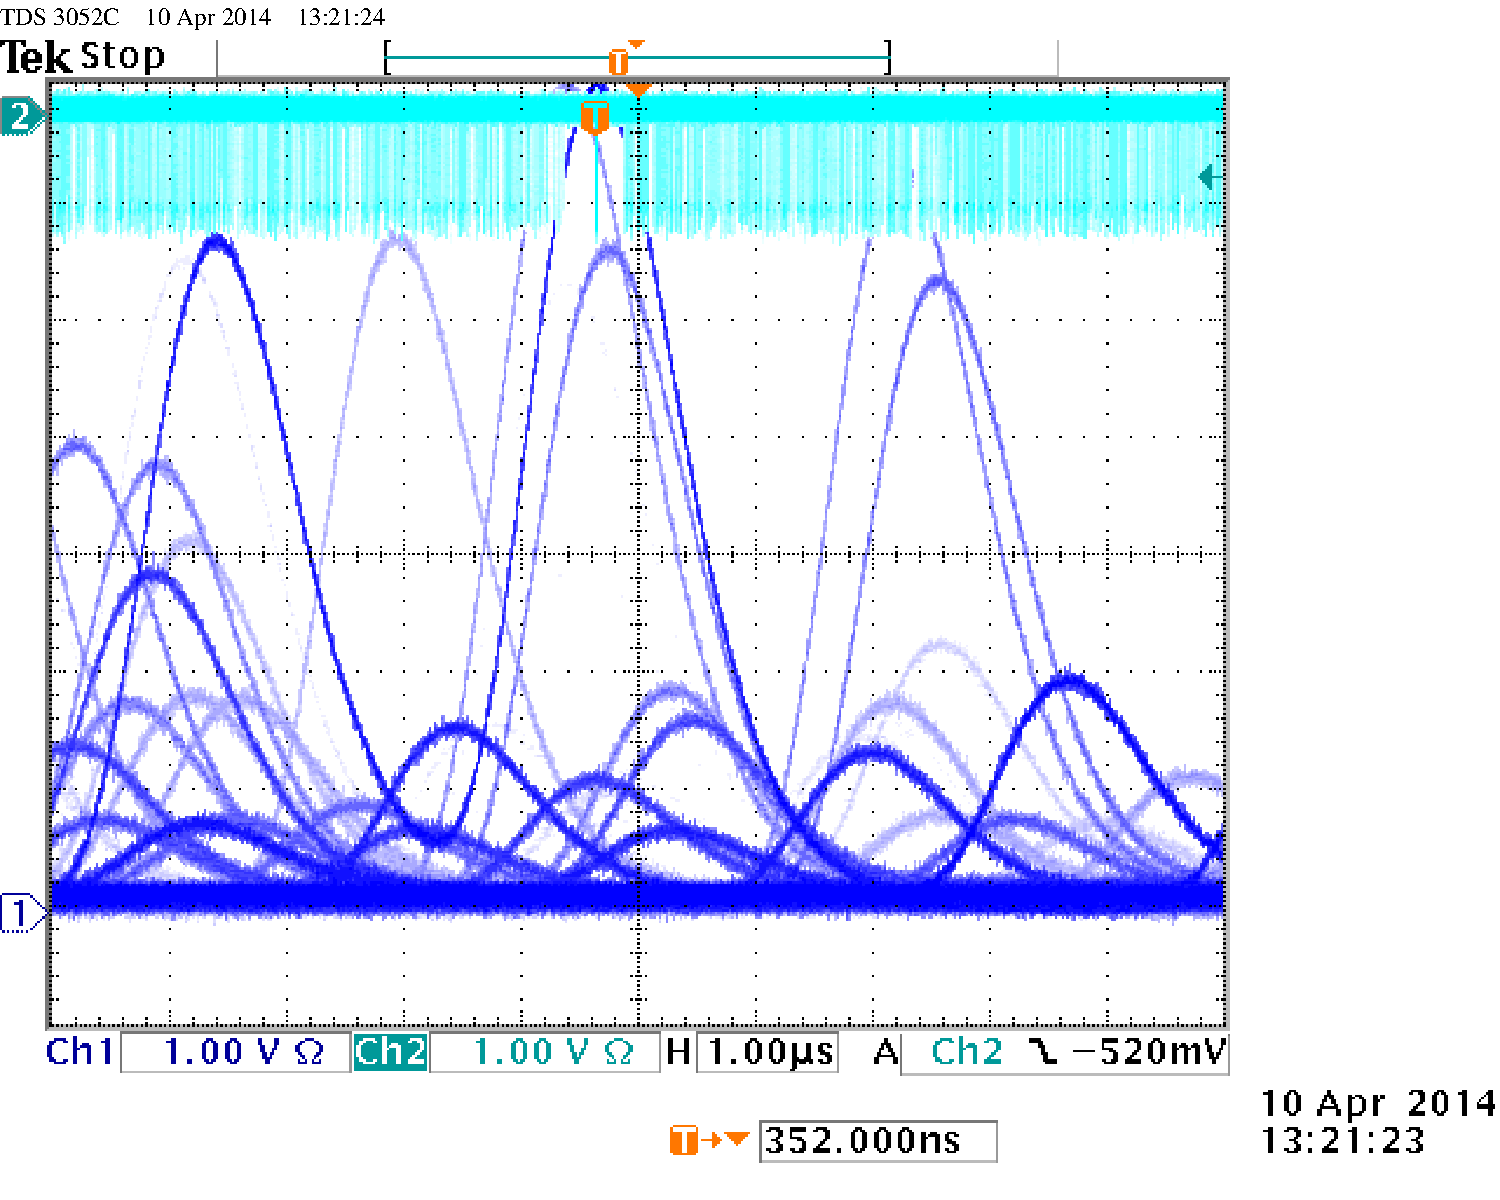
\includegraphics[width=0.49\linewidth]{../Daten/2014-04-10_13-21-east.pdf}
    \hfill
    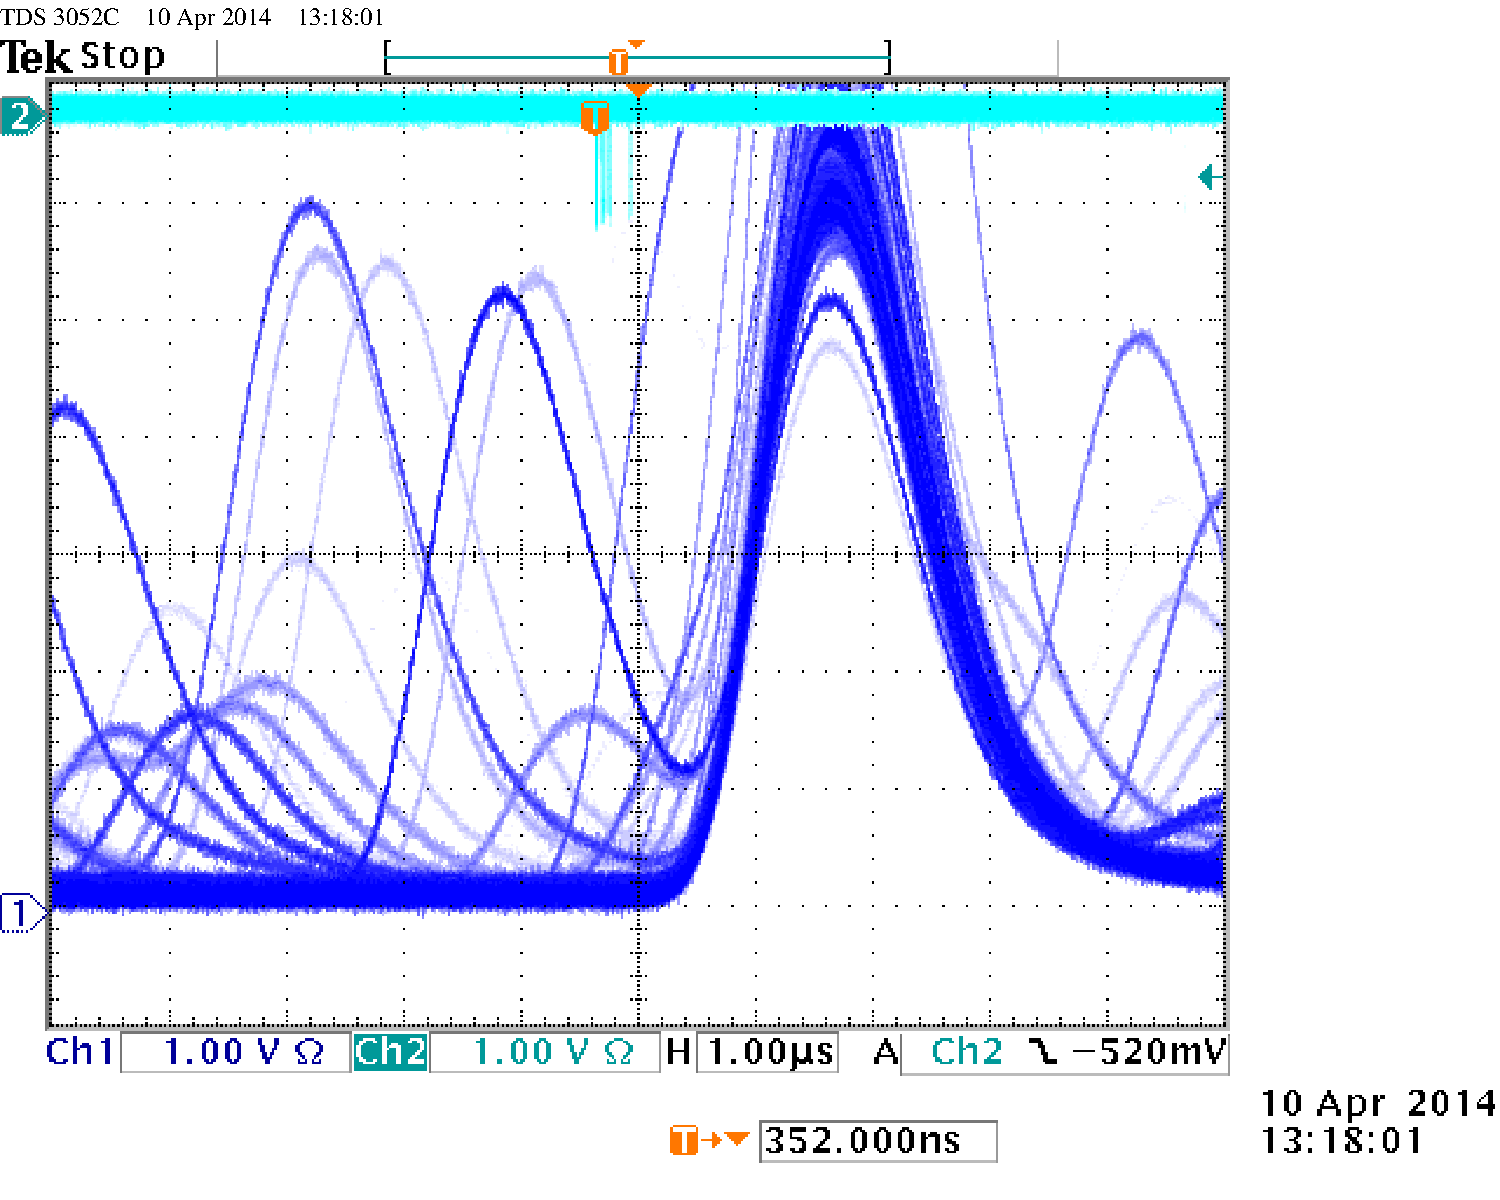
\includegraphics[width=0.49\linewidth]{../Daten/2014-04-10_13-18-east.pdf}
    \caption{%
        Stop- und Start-Signal der CFDs zusammen mit ihren Slow-Signalen.
    }
    \label{fig:ba_start_slow_baseline}
\end{figure}

Beim Start-Zweig ist die untere Grenze schon ausreichend hoch, um den
Untergrund zu filtern.

\begin{figure}[htbp]
    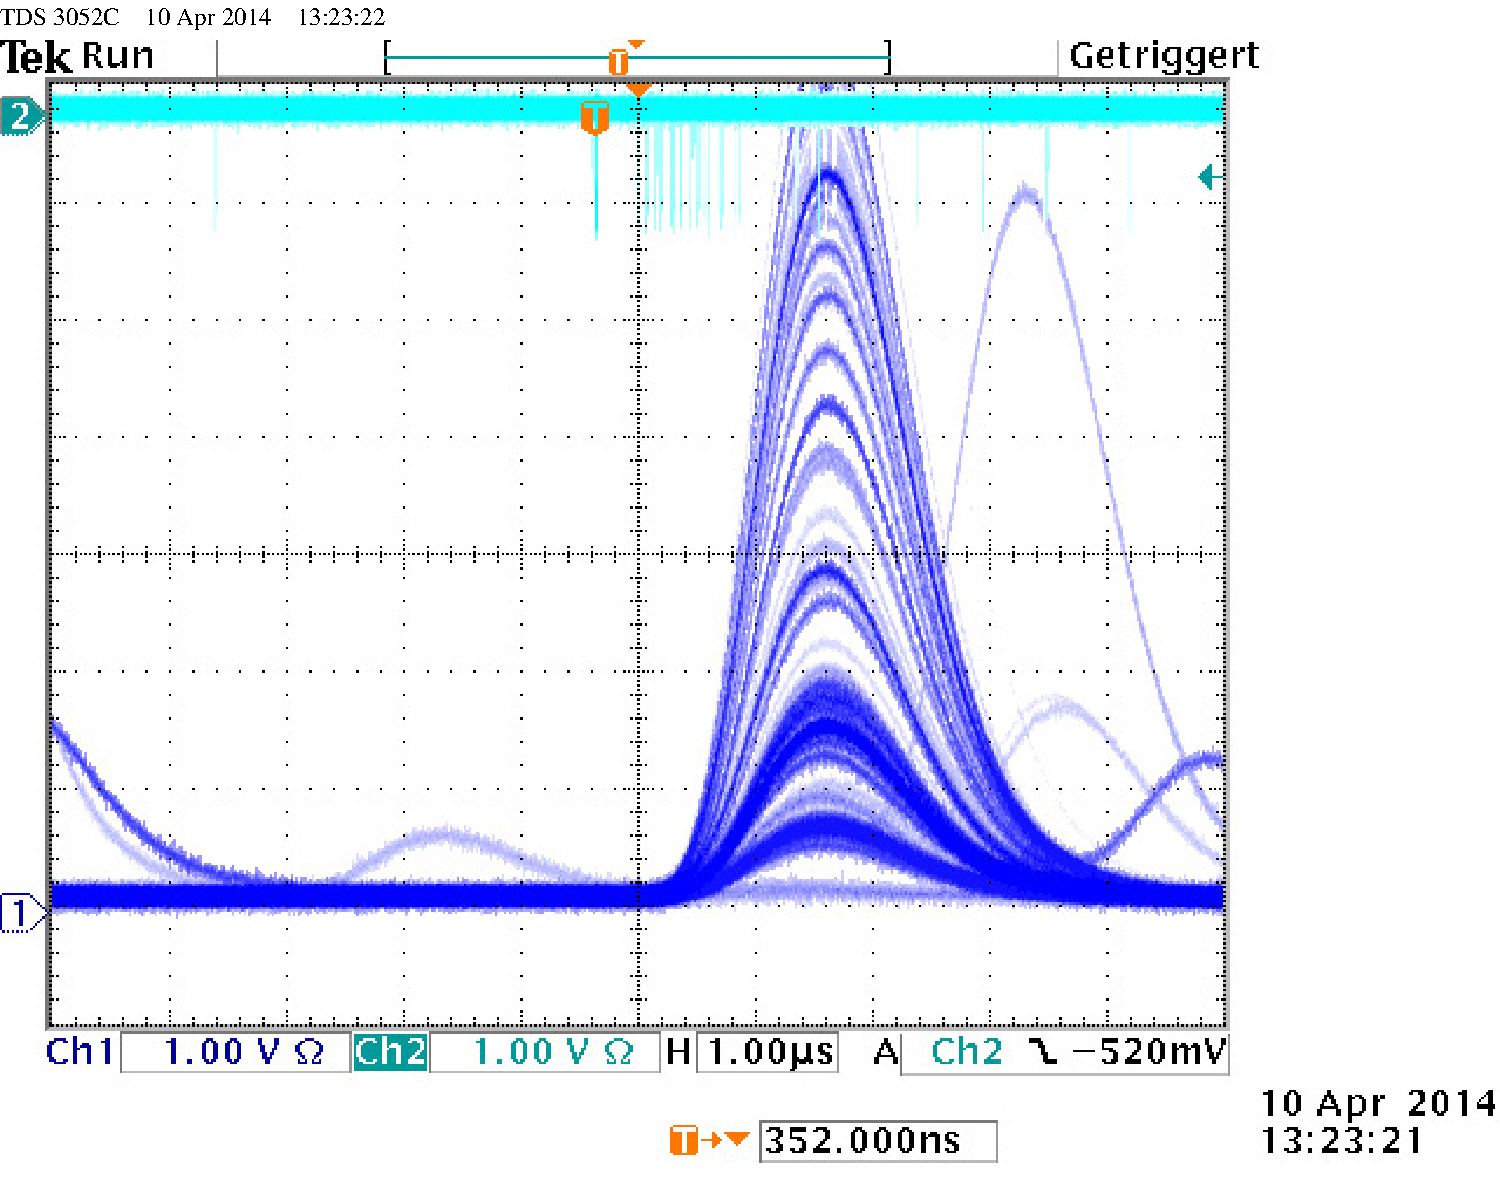
\includegraphics[width=0.49\linewidth]{../Daten/2014-04-10_13-23-east.pdf}
    \caption{%
        Stop-Signal zusammen mit seinem Slow-Signal, mit höherer Schwelle.
    }
    \label{fig:ba_start_slow}
\end{figure}

Wir überprüfen nun die Fast-Koinzidenz, indem wir Start- und Stop-Signal am
Oszilloskop betrachten. Ein Beispiel für den Fast-Abgleich /* Bildzeit 13:54 */
ist in Abbildung~\ref{fig:fast_abgleich_oszi}. Wir müssen darauf achten, dass
das Start-Signal (Kanal 1) in den meisten Fällen vor dem Stop-Signal (Kanal 2)
kommt. Damit dies immer der Fall ist, schalten wir eine ausreichende
Verzögerung hinter den Stop-CFD.

\begin{figure}[htbp]
    \centering
    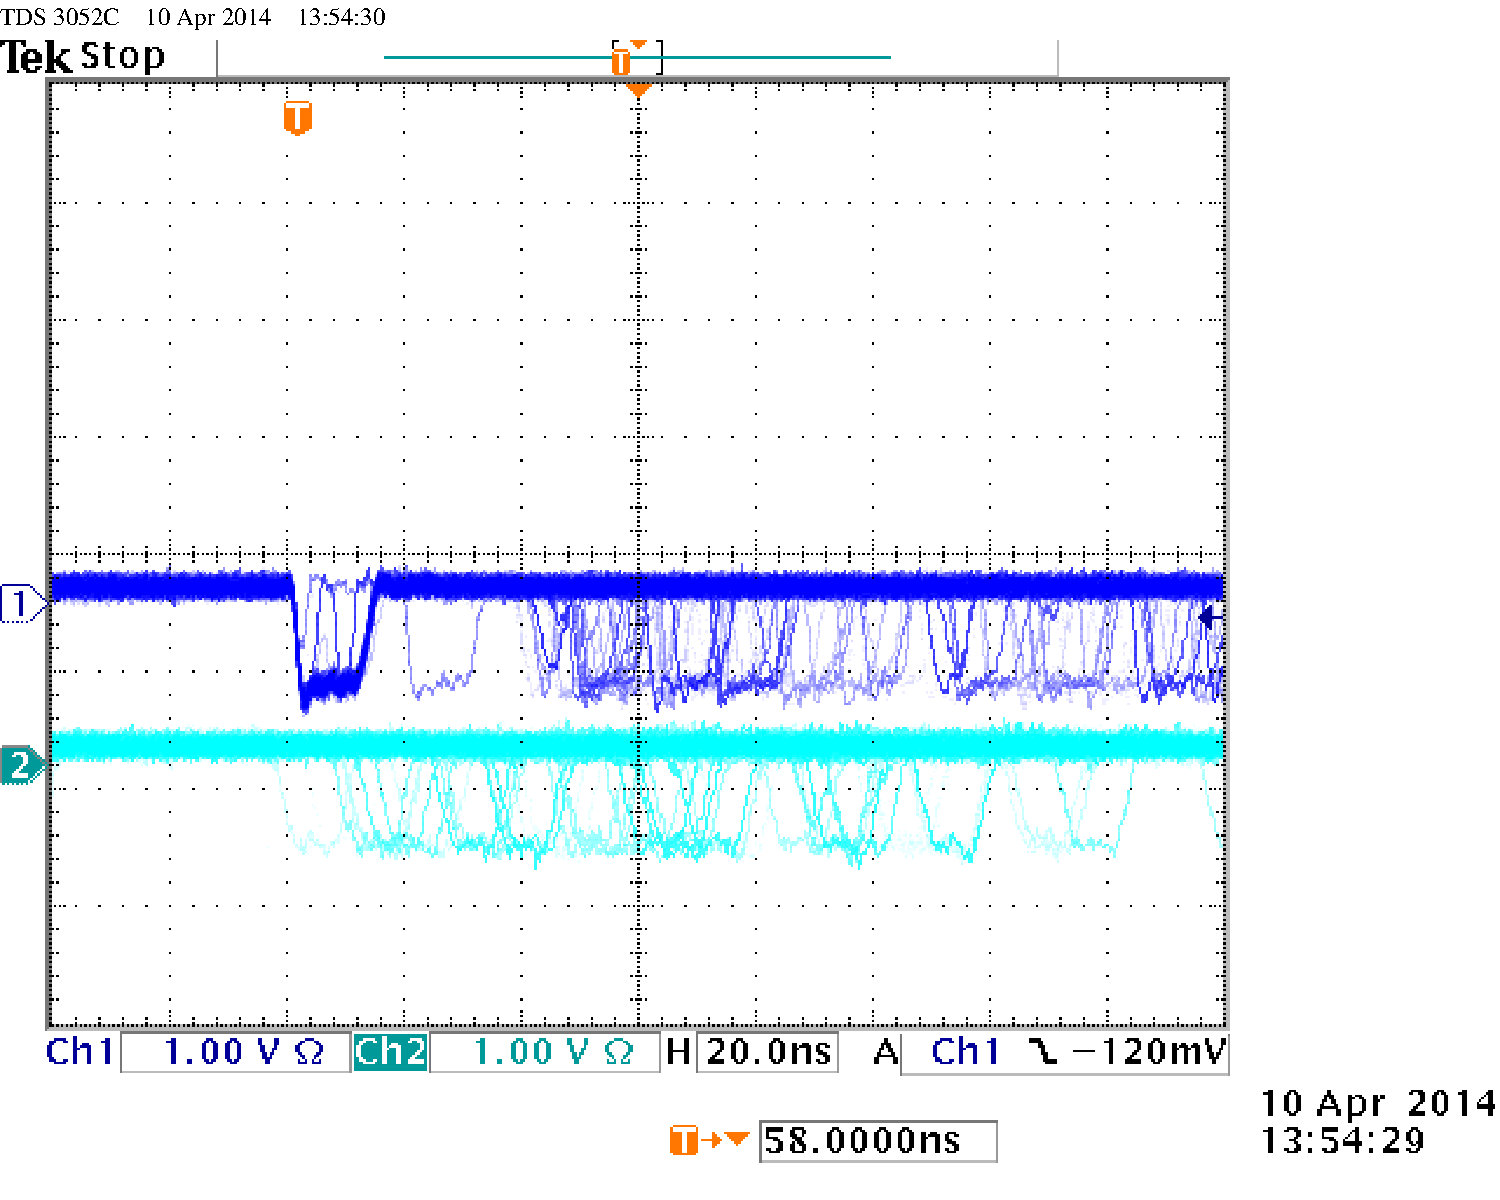
\includegraphics[width=0.49\linewidth]{../Daten/2014-04-10_13-54-east.pdf}
    \caption{%
        Abgleich der beiden Fast-Zweige.
    }
    \label{fig:fast_abgleich_oszi}
\end{figure}

Wir stellen die CFD Schwelle nach dem Skript ein, indem wir das Slow-Signal
und negatives Stop-CFD Signal auf das MCA geben. Die Schwelle des Stop-CFD
stellen wir so, dass die für die Röntgenlinie keine Ereignisse mehr registriert
werden/* 013 */, siehe Abbildung~\ref{mca:xray}.

\begin{figure}[htbp]
    \centering
    \begin{tikzpicture}
        \begin{axis}[
                width=\linewidth, height=0.3\linewidth, xlabel=Kanal,
                ylabel=Ereignisse, axis lines=left, xtick={0,1000,...,8000}
            ]
            \addplot[black] table {../Daten/013-Ba-CFD-l.txt};
        \end{axis}
    \end{tikzpicture}
    \caption{%
        Spektrum des Barium. Hiermit haben wir die Schwelle für das Stop-CFD
        eingestellt, so dass die Röntgenlinie nicht mehr auslöst.
    }
    \label{mca:xray}
\end{figure}

Wir tauschen kurz die Barium gegen Natrium, um zu überprüfen, ob die
\SI{511}{\kilo\electronvolt}-Linie noch an der richtigen Stelle im MCA ist.
Dies ist der Fall. Somit stimmt unsere Energieeichung noch.

Wir machen den Abgleich Fast- und Slow-Koinzidenz auf dem Oszilloskop/* Bildzeit
13:53 */, siehe Abbildung~\ref{fig:fast-slow-abgleich}.

\begin{figure}[htbp]
    \centering
    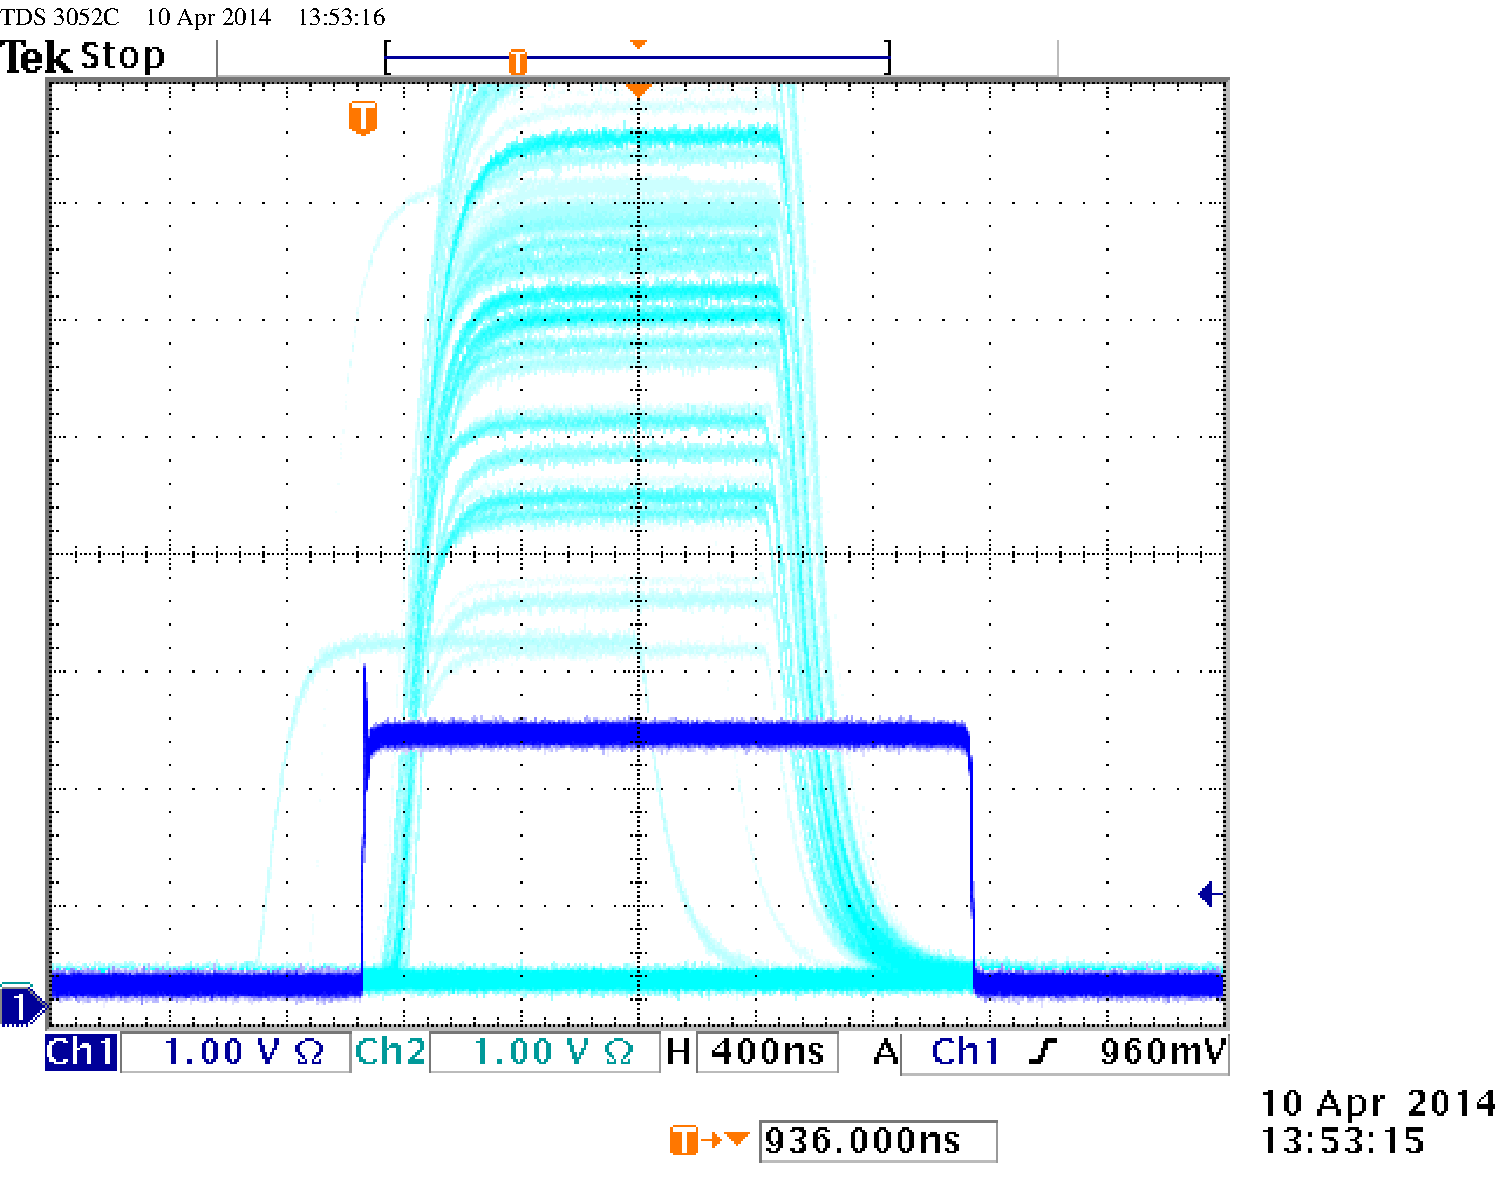
\includegraphics[width=0.49\linewidth]{../Daten/2014-04-10_13-53-east.pdf}
    \caption{%
        Abgleich von Fast- und Slow-Koinzidenz.
    }
    \label{fig:fast-slow-abgleich}
\end{figure}

Nun ist der Aufbau fertig für die Bariumquelle kalibriert und wir können mir
der Lebensdauermessung starten, die über Nacht geht.

\nocite{Bieling/K125}
\nocite{Leo/Techniques_Nuclear_Experiments}


\chapter{Auswertung}

\begin{figure}[htbp]
    \centering
    \begin{tikzpicture}
        \begin{axis}[width=0.45\linewidth, height=0.3\linewidth, xlabel=Kanal, ylabel=Ereignisse, axis lines=left]
            \addplot[black] table {../Daten/005-Na-Zoom.txt};
            \addplot[red, very thick] table {fit_Na_links_511.txt};
        \end{axis}
    \end{tikzpicture}
    \hfill
    \begin{tikzpicture}
        \begin{axis}[width=0.45\linewidth, height=0.3\linewidth, xlabel=Kanal, ylabel=Ereignisse, axis lines=left]
            \addplot[black] table {../Daten/003-Na-Spektrum.txt};
            \addplot[red, very thick] table {fit_Na_rechts_511.txt};
        \end{axis}
    \end{tikzpicture}
    \caption{%
        Anpassungskurven an die Spektren der Na-Probe im rechten und linken
        Detektor.
    }
    \label{}
\end{figure}

\begin{figure}[htbp]
    \centering
    \begin{tikzpicture}
        \begin{axis}[width=0.45\linewidth, height=0.3\linewidth, xlabel=Kanal, ylabel=Ereignisse, axis lines=left]
            \addplot[black] table {../Daten/011-Ba-Spek-l.txt};
            \addplot[red, very thick] table {fit_Ba_links_31.txt};
            \addplot[red, very thick] table {fit_Ba_links_81.txt};
            \addplot[red, very thick] table {fit_Ba_links_356.txt};
        \end{axis}
    \end{tikzpicture}
    \hfill
    \begin{tikzpicture}
        \begin{axis}[width=0.45\linewidth, height=0.3\linewidth, xlabel=Kanal, ylabel=Ereignisse, axis lines=left]
            \addplot[black] table {../Daten/009-Ba-Spek-r.txt};
        \end{axis}
    \end{tikzpicture}
    \caption{%
        Spektrum der Bariumemissionen im linken und rechten Detektor.
    }
    \label{}
\end{figure}

\chapter{Ergebnis}

\IfFileExists{\bibliographyfile}{
    \printbibliography
}{}

\end{document}

% vim: spell spelllang=de tw=79
